\section{Theorem \ref{thm:oodom-guarantee}}
\label{sec:proofs_007}

We prove theorem \ref{thm:oodom-guarantee} based on Lemmas \ref{lem:relu-regions_007} and \ref{lem:limit-not-density}. Lemma \ref{lem:relu-regions_007} states that the input space can be divided in a finite number of linear regions \citep{understanding-nn-relu}. Lemma \ref{lem:limit-not-density} states that a probability density with bounded derivatives has to converge to $0$ at infinity \citep{limit-existence-infinity}. We additionally recall Lemma \ref{lem:limit-density} which provide a similar convergence guarantee without the bounded derivative constraint \citep{integrable-infinity}. Finally, Lemma \ref{lem:limit-gmm-radial} particularly shows that the guarantee of theorem 1 can be obtained with Gaussian Mixtures which are commonly used for density estimation or radial flows which are used in the experiments.

\begin{lemma}
\label{lem:relu-regions_007}
\citep{understanding-nn-relu} Let $\{Q_l\}_l^{R}$ be the set of linear regions associated to the piecewise ReLU network $f_{\phi}(\x)$. For any $\x \in \real^\inputdim$, there exists $\delta^* \in \real^{+}$ and $l^*\in {1,..., R}$ such that $\delta \x \in Q_{l^*}$ for all $\delta > \delta^*$.
\end{lemma}

\begin{lemma}
\label{lem:limit-not-density}
\citep{limit-existence-infinity} Let $p \in L^1(0, \infty)$ with bounded first derivative $p'$, then $p(\delta)\underset{\delta \rightarrow \infty}{\rightarrow} 0$. This convergence is stronger than in Lem.~\ref{lem:limit-density} as the limit is not in density but with standard limit notation.
\end{lemma}

\begin{lemma}
\label{lem:limit-density}
\citep{integrable-infinity} Let $p \in L^1(0, \infty)$, then $p(\delta)\underset{\delta \rightarrow \infty}{\rightarrow} 0$ in density. This means that the sets where $p(t)$ is far from its $0$ limit (i.e. $\{ t \geq 0: |p(t)| \geq \epsilon \}$ with $\epsilon > 0$) has zero density.
\end{lemma}

\begin{lemma}
\label{lem:limit-gmm-radial}
Let $\prob(\z \condition \bm{\omega})$ be parametrized with a Gaussian Mixture Model (GMM) or a radial flow, then $\prob(\z \condition \bm{\omega})\underset{||\z|| \rightarrow \infty}{\rightarrow} 0$.
\end{lemma}
\begin{proof}
We prove now lem.~\ref{lem:limit-gmm-radial} for GMM and radial flow. The proof is straightforward for the GMM parametrization since every Gaussian component of the mixture has $0$ limit when $||\z|| \rightarrow \infty$.

Let denote now $p_1(z) = \prob(\z \condition \bm{\omega})$ be parametrized with a radial flow transformation $g(\z)$ and a base unit Gaussian distribution $p_0$ i.e.:
\begin{align*}
    p_1(\z) = p_0(g(\z)) \times |\text{det}\frac{\partial g(\z)}{\partial\z}|
\end{align*}
Further, we can express the transformation $g(\z)$ and its determinant $\text{det}\frac{\partial g(z)}{\partial\z}$ as follows:
\begin{align*}
    g(\z) &= \z + \beta h(\alpha, r) (\z - \z_0)\\
    \text{det}\frac{\partial g(z)}{\partial\z} &= \frac{1+\beta h(\alpha, r)+\beta h'(\alpha, r)r}{(1 + \beta h(\alpha, r))^{\latentdim-1}}
\end{align*}
where $h(\alpha, r) =\frac{1}{\alpha + r}$ and $r=||\z - \z_0||$. On one hand, we have $||g(\z)|| \rightarrow +\infty$ when $||\z|| \rightarrow \infty$ since $||\beta h(\alpha, r) (\z - \z_0)|| < \beta$. Thus, the base Gaussian density $p_0(g(\z))\rightarrow 0$ when $||\z|| \rightarrow \infty$. On the other hand, we have $|\text{det}\frac{\partial g(z)}{\partial\z}|\rightarrow 1$ since $\beta h(\alpha, r) \rightarrow 0$ and $\beta h'(\alpha, r)r \rightarrow 0$ when $||\z|| \rightarrow \infty$. Therefore, the transformed density $p_0(g(\z)) \times |\text{det}\frac{\partial g(\z)}{\partial\z}| \rightarrow 0$ when $||\z|| \rightarrow \infty$ which ends the proof. Note that this proof can be extended to stacked radial flows by induction.
\end{proof}

\begin{theorem*}
Let a \NatPNacro{} model parametrized with a (deep) encoder $f_{\phi}$ with piecewise ReLU activations, a decoder $g_{\psi}$ and the density $\prob(\z \condition \bm{\omega})$. Let $f_{\phi}(\x)= V^{(l)}\x + a^{(l)}$ be the piecewise affine representation of the ReLU network $f_{\phi}$ on the finite number of affine regions $Q^{(l)}$ \citep{understanding-nn-relu}. Suppose that $V^{(l)}$ have independent rows and the density function $\prob(\z \condition \bm{\omega})$ has bounded derivatives, then for almost any $\x$ we have \smash{$\prob(f_{\phi}(\delta \cdot \x) \condition \bm{\omega}) \underset{\delta \rightarrow \infty}{\rightarrow} 0$}. i.e the evidence becomes small far from training data.
\end{theorem*}

\begin{proof}
We prove now thm.~\ref{thm:oodom-guarantee}. Let $\x \in \real^\inputdim $ be a non-zero input and $f_{\phi}$ be a ReLU network. Lem.~\ref{lem:relu-regions_007} implies that there exists $\delta^* \in \real^{+}$ and $l \in \{1,..., R\}$ such that $\delta \cdot \x \in Q^{(l)}$ for all $\delta > \delta^*$. Thus, $\z_{\delta} = f_{\phi}(\delta \cdot \x) = \delta \cdot (V^{(l)} \x) + a^{(l)}$ for all $\delta > \delta^*$. Note that for $\delta\in [\delta^*, +\infty]$,  $\z_{\delta}$ follows an affine half line $S_{\x} = \{\z \condition \z = \delta \cdot (V^{(l)} \x) + a^{(l)}, \delta > \delta^* \}$ in the latent space. Further, note that $V^{(l)}\x \neq 0$ and $|| \z_\delta|| \underset{\delta \rightarrow \infty}{\rightarrow} + \infty$ since $\x \neq 0$ and $V^{(l)}$ has independent rows.

We now define the function $p(\delta)=\prob(\z_{\delta} \condition \bm{\omega})$ which is the density function $\prob(\z \condition \bm{\omega})$ restricted on the affine half line $S_{\x}$. Since $\prob(\z \condition \bm{\omega})$ is a normalized probability density, then the function $\delta \mapsto p(\delta - \delta^*)$ is integrable on $[0, +\infty]$. Indeed we have:
\begin{align*}
    \int_{0}^{+\infty} p(\delta - \delta^*) d\delta &= \int_{\delta^*}^{+\infty} p(\delta) d\delta \\
    &= \int_{\delta^*}^{+\infty} \prob(\delta \cdot (V^{(l)} \x) + a^{(l)} \condition \bm{\omega}) d\delta\\
    &= \int^{S_{\x}} \prob(\z \condition \bm{\omega}) d\z < +\infty
\end{align*}
Further since the function $\prob(\z \condition \bm{\omega})$ has bounded derivatives, we can apply  Lem.~\ref{lem:limit-not-density} to the function $\delta \mapsto p(\delta - \delta^*)$ to get the expected result i.e.
\begin{align*}
    \prob(f_{\phi}(\delta \cdot \x) \condition \bm{\omega}) = p(\delta) = p((\delta + \delta^*) - \delta^*) \underset{\delta \rightarrow \infty}{\rightarrow} 0
\end{align*}
which ends the proof.

Alternatively a slightly weaker conclusion also holds if the density function does not have bounded derivatives using lem.~\ref{lem:limit-density} (instead of lem.~\ref{lem:limit-not-density}) with the notion of limit in density. The stronger conclusion is valid if we parametrize $\prob(\z \condition \bm{\omega})$ with a Gaussian Mixture Model or a radial flow density according to lem.~\ref{lem:limit-gmm-radial} since $|| \z_\delta|| \underset{\delta \rightarrow \infty}{\rightarrow} + \infty$.
\end{proof}

Further, we provide additional comments on the assumption that a trained network converges to linear transformation with exactly two or more dependent rows in Thm.~\ref{thm:oodom-guarantee}. Under this realistic condition \cite{overconfident-relu}, the null space is reduced to $0$ according to the rank-nullity theorem meaning that there should be no dead input feature/pixel. If this condition does not hold, this would mean that this specific input feature/pixel is not informative for the prediction task. Thus it could be desired in practice that it does not affect the uncertainty on the prediction. This latter aspect is discussed in the “Task-Specific OOD” paragraph in Sec.~\ref{sec:limitations}.

\section{Bayesian Loss} 
\label{sec:loss}

\NatPNacro{} minimizes the following Bayesian formulation:
%
\begin{equation}
    \mathcal{L}\dataix = - \underbrace{\expectation_{\expparam\dataix \sim \prior^{\text{post},(\idata)}}[\log \prob(\y\dataix\condition \expparam \dataix)]}_\text{(i)} - \underbrace{\entropy[\prior^{\text{post},(\idata)}]}_\text{(ii)}
\end{equation}
%
where $\entropy[\prior^{\text{post},(\idata)}]$ denotes the entropy of the predicted posterior distribution $\prior^{\text{post},(\idata)}$. This loss is generally not equal to the ELBO loss. While the term \textbf{(i)} can be viewed as an ELBO loss without KL regularization, the term \textbf{(ii)} is not necessarily equal to the prior KL regularization term in the ELBO loss since a proper uniform prior might not exist (e.g. the target $\y$ is a real number). Indeed, if the target $y$ is a real number, there exists no uniform prior on $\expparam$ and the Bayesian loss and ELBO loss are different i.e. $KL(\prior||\prior^\text{prior}) = \int \prior(\theta) \log (\frac{\prior(\theta)}{\prior^\text{prior}(\theta)}) d\theta \neq \int \prior(\theta) \log \prior(\theta) d\theta = \entropy(\prior)$. Nonetheless, when a uniform prior $\prior^\text{unif}$ exists (e.g. the target $\y$ is a class), the loss optimization can be seen as an amortized variational optimization of an ELBO loss \citep{amortized-variational-inference} i.e. $\mathcal{L}\dataix = - \expectation_{\prior^{\text{post},(\idata)}}[\log \prob(\y\dataix\condition \expparam \dataix)] + \text{KL}[\prior^{\text{post},(\idata)}\|\prior^\text{unif}]$ where the predicted distribution $\prior^{\text{post},(\idata)}$ is the variational distribution --- which approximates the true posterior distribution. Indeed, the KL regularization term is equal to the entropy regularization term i.e. $KL(\prior||\prior^\text{unif}) = \int \prior(\theta) \log (\frac{\prior(\theta)}{\prior^\text{unif}(\theta)} d\theta) \propto \int \prior(\theta) \log Q(\theta) d\theta) = \entropy(\prior)$. Hence, the loss name ``Bayesian loss'' \citep{charpentier2020} is motivated by its difference with the ELBO loss and its Bayesian property at optimum.

\section{Formulae for Exponential Family Distributions}
\label{sec:formulae}

\subsection{General Case}

\textbf{Target Distribution.} An exponential family distribution on a target variable $\y \in \real$ with natural parameters $\expparam \in \real^\suffstatdim$ can be denoted as
%
\begin{equation} \label{eq:exp-family}
    \prob(\y \condition \expparam) = h(\y) \exp\left(\expparam^T \bm{u}(\y) - A(\expparam)\right)
\end{equation}
%
where ${h: \real \rightarrow \real}$ is the carrier measure, ${A: \real^\suffstatdim \rightarrow \real}$ the log-normalizer and ${\bm{u}: \real \rightarrow \real^\suffstatdim}$ the sufficient statistics.

\textbf{Conjugate Prior Distribution.} An exponential family distribution $\prob$ always admits a conjugate prior:
%
\begin{equation}\label{eq:conj-prior}
    \prior(\expparam \condition \priorparam, \evidence) = \eta(\priorparam, \evidence) \exp\left( \evidence \, \bm{\theta}^T\priorparam  - \evidence A(\expparam) \right)
\end{equation}
%
where $\eta : \real^L \times \real \rightarrow \real$ is a normalization factor and $A$ the log-normalizer of the distribution $\prob$ as in Eq.~\ref{eq:exp-family}).

\textbf{Posterior Predictive Distribution.} The posterior predictive distribution is given as $\int \prob(\y\dataix|\expparam)\prior(\expparam|\priorparam^{\text{post}, (i)}, \evidence^{\text{post}, (i)}) d\expparam$ where the parameter $\expparam$ is marginalized out  \citep{uncertainty-deep-learning}. This distribution can always be computed in closed form for exponential family distributions:
%
\begin{align}
\prob(\y \condition \priorparam, \evidence) = h(\y) \frac{\eta(\priorparam, \evidence)}{\eta\left(\frac{\evidence \priorparam + \bm{u}(\y)}{\evidence +1}, \evidence + 1 \right)}
\end{align}
%
where $h$ is the carrier measure defined in Eq.~\ref{eq:exp-family} and $\eta$ is the normalization factor defined in Eq.~\ref{eq:conj-prior}. In particular, the posterior predictive distributions for Categorical, Normal and Poisson target distributions are Categorical, Student and Negative Binomial distributions, respectively.

\textbf{Likelihood.} The log-likelihood of an exponential family distribution can be written as follows:
%
\begin{equation}\label{eq:log-likelihood}
    \log{\prob(\y\dataix \condition \bm{\expparam})} = \log{h(\y\dataix)} + \expparam^T \bm{u}(y\dataix) - A(\expparam)
\end{equation}

\textbf{Expected Log-Likelihood.} Given the log-likelihood of an exponential family distribution, its expectation under the conjugate prior distribution $\prior(\expparam|\priorparam, \evidence)$ can be written as
%
\begin{equation}\label{eq:expected-log-likelihood}
    \expectation_{\expparam \sim \prior(\priorparam, \evidence)}[\log{\prob(\y\dataix \condition \bm{\expparam})}] = \log{h(\y\dataix)} + \expectation_{\expparam \sim \prior(\priorparam, \evidence)}[\expparam]^T \bm{u}(y\dataix) - \expectation_{\expparam \sim \prior(\priorparam, \evidence)}[A(\expparam)]
\end{equation}
%
where $\expectation_{\prior(\expparam|\priorparam, \evidence)}[\expparam] = \priorparam$ \citep{exponential-family-stats, conjugate-prior-exponential-family}.

\textbf{Entropy.} The entropy of a random variable $\y \sim \prob(\y | \expparam)$ for an exponential family distribution $\prob$ can be written as follows \citep{exponential-entropy}:
%
\begin{equation}
    \entropy[\prob(\y | \expparam)] = A(\expparam) - \expparam^T \nabla_{\bm{\theta}}A(\expparam) - \expectation_{y \sim \prob(\expparam)}[\log{h(\y)}]
\end{equation}

%%%%%%%%%%%%%%%%%%%%%%%%%%%%%%%%%%%%%%%%%%%%%%%%%%%%%%%%%%%%%%%%%%%%%%%%%%%%%%%%%%%%%%%%

\subsection{Categorical \& Dirichlet Distributions}

The Dirichlet distribution $\bm{p} \sim \DDir(\bm{\alpha})$ is the conjugate prior of the categorical distributions $\bm{\y} \sim \DCat(\bm{p})$.

\textbf{Target Distribution.} The density and the entropy of the categorical distribution are:
%
\begin{align}\label{eq:density-entropy-categorical}
    &\DCat(\y \condition \bm{p}) = \sum_{i=1}^K{\mathbb{I}[\y_i = 1] \, p_i} \\
    &\entropy[\DCat(\bm{p})] = \sum_{\iclass=1}^\nclass{\log{p_\iclass}}
\end{align}

\textbf{Conjugate Prior Distribution.} The density and the entropy of the Dirichlet distribution are:
%
\begin{align}\label{eq:density-entropy-dirichlet_007}
        &\DDir(\bm{p} \condition \bm{\alpha}) = \frac{\Gamma\left(\sum_{\iclass=1}^\nclass{\alpha_\iclass}\right)}{\prod_{\iclass=1}^K{\Gamma(\alpha_\iclass)}} \prod_{\iclass=1}^\nclass{p_\iclass^{\alpha_\iclass-1}}\\
        &\entropy[\DDir(\bm{\alpha})] = \log B(\bm{\alpha}) + (\alpha_0 - \nclass) \psi(\alpha_0) - \sum_\iclass (\alpha_\iclass - 1) \psi(\alpha_\iclass)
\end{align}
%
where $\psi(\alpha)$ and $B(\bm{\alpha})$ denote Digamma and Beta functions, respectively, and $\alpha_0 = \sum_{c}{\alpha_c}$.

\textbf{Expected Log-Likelihood.} The expected likelihood of the categorical distribution $\DCat(\bm{p})$ under the Dirichlet distribution $\DDir(\bm{\alpha})$ is
%
\begin{align}\label{eq:expected-likelihood-cat-dir_007}
    \expectation_{\bm{p} \sim \DDir(\bm{\alpha})}[\log \DCat(\y \condition \bm{p})] = \psi(\alpha_{\y}) - \psi(\alpha_0)
\end{align}
%
where $\psi(\alpha)$ denotes Digamma function.

%%%%%%%%%%%%%%%%%%%%%%%%%%%%%%%%%%%%%%%%%%%%%%%%%%%%%%%%%%%%%%%%%%%%%%%%%%%%%%%%%%%%%%%%

\subsection{Normal \& Normal-Inverse-Gamma Distributions}

The Normal-Inverse-Gamma (NIG) distribution $\mu, \sigma \sim \DNIG(\mu_0, \lambda, \alpha, \beta)$ is the conjugate prior of the normal distribution $\y \sim \DNormal(\mu, \sigma)$. Note that as both parameters $\lambda$ and $\alpha$ can be viewed as pseudo-counts. However, the natural prior parametrization enforces a single pseudo-count $\evidence$ corresponding to $\lambda = 2 \alpha$.

\textbf{Target Distribution.} The density and the entropy of the Normal distribution are:
%
\begin{align}\label{eq:density-entropy-normal}
    &\DNormal(\y \condition \mu, \sigma) = \frac{1}{\sigma \sqrt{2\pi}} \exp\left( -\frac{(x - \mu)^2}{2\sigma^2} \right)\\
    &\entropy[\DNormal(\mu, \sigma)] = \frac{1}{2}\log(2\pi\sigma^2)
\end{align}

\textbf{Conjugate Prior Distribution.} The density and the entropy of the NIG distribution are:
%
\begin{align}\label{eq:density-entropy-nig}
    &\DNIG(\mu, \sigma \condition \mu_0, \lambda, \alpha, \beta) = \frac{\beta^\alpha \sqrt{\lambda}}{\Gamma(\alpha) \sqrt{2\pi\sigma^2}} \left(\frac{1}{\sigma^2}\right)^{\alpha+1} \exp\left( - \frac{2\beta + \lambda (\mu - \mu_0)^2}{2 \sigma^2}\right)\\
    &\entropy[\DNIG(\mu_0, \lambda, \alpha, \beta)] = \frac{1}{2} + \log\left((2\pi)^{\frac{1}{2}}\beta^{\frac{3}{2}}\Gamma(\alpha)\right) - \frac{1}{2} \log{\lambda} + \alpha - \left(\alpha+\frac{3}{2}\right)\psi(\alpha)
\end{align}
%
where $\Gamma(\alpha)$ denotes the Gamma function.

\textbf{Expected Log-Likelihood.} The expected likelihood of the Normal distribution $\DNormal(\mu, \sigma)$ under the NIG distribution $\DNIG(\mu_0, \lambda, \alpha, \beta)$ is:
%
\begin{align}\label{eq:expected-likelihood-normal-nig}
\expectation_{(\mu, \sigma) \sim \DNIG(\mu, \lambda, \alpha, \beta)}&[\log \DNormal(\y \condition \mu, \sigma)] \\
&= \expectation\left[-\frac{(y-\mu)^2}{2\sigma^2} - \log(\sigma\sqrt{2\pi}) \right]\\
&= \frac{1}{2}\left(-\expectation\left[ \frac{(y-\mu_0)^2}{2\sigma^2} \right] - \expectation\left[ \log\sigma^2 \right] - \log2\pi \right)\\
&= \frac{1}{2}\left(-\y^2\expectation\left[ \frac{1}{\sigma^2} \right] + 2 \y \expectation\left[\frac{\mu}{\sigma^2}\right] - \expectation\left[ \frac{\mu^2}{\sigma^2} \right] + \expectation\left[ \log\frac{1}{\sigma^2} \right] - \log2\pi \right)\\
&= \frac{1}{2}\left(- \frac{\alpha}{\beta} (\y - \mu_0)^2 - \frac{1}{\lambda} + \psi(\alpha) - \log{\beta} - \log{2\pi}\right)
\end{align}
%
where $\psi(\alpha)$ denotes the Digamma function. We used here the moments of the NIG distribution $\expectation\left[\frac{\mu}{\sigma^2}\right]=\frac{\alpha \mu_0}{\beta}$, $\expectation\left[\frac{1}{\sigma^2}\right]=\frac{\alpha}{\beta}$, $\expectation\left[\frac{\mu^2}{\sigma^2}\right]=\frac{\alpha \mu_0^2}{\beta} + \frac{1}{\lambda}$, and the moment of the inverse Gamma distribution $\expectation\left[\log{\frac{1}{\sigma^2}}\right]=\psi(\alpha) - \log{\beta}$.

%%%%%%%%%%%%%%%%%%%%%%%%%%%%%%%%%%%%%%%%%%%%%%%%%%%%%%%%%%%%%%%%%%%%%%%%%%%%%%%%%%%%%%%%

\subsection{Poisson \& Gamma Distributions}

The Gamma distribution $\lambda \sim \DGamma(\alpha, \beta)$ is the conjugate prior of the Poisson distributions $\y \sim \DPoi(\lambda)$. 

\textbf{Target Distribution.} The density and the entropy of the Poisson distribution are:
%
\begin{align}\label{eq:density-entropy-poisson}
    &\DPoi(\y \condition \lambda) = \frac{\lambda^\y \exp(-\lambda)}{\y!}\\
    &\entropy[\DPoi(\lambda)] = \lambda(1 - \log(\lambda))) + \exp(-\lambda)\sum_{k=0}^{\infty}\frac{\lambda^k\log(k!)}{k!}
\end{align}

\textbf{Conjugate Prior Distribution.} The density and the entropy of the Gamma distribution are:
%
\begin{align}\label{eq:density-entropy-gamma}
        &\DGamma(\lambda \condition \alpha, \beta) = \frac{\beta^\alpha}{\Gamma(\alpha)} \lambda^{\alpha - 1}\exp(-\beta \lambda)\\
        &\entropy[\DGamma(\alpha, \beta)] = \alpha + \log{\Gamma(\alpha)} - \log{\beta} + (1 - \alpha) \psi(\alpha)
\end{align}
%
where $\Gamma(\alpha)$ denotes the Gamma function.

\textbf{Expected Log-Likelihood.} The expected likelihood of the Poisson distribution $\DPoi(\lambda)$ under the Gamma distribution $\DGamma(\alpha, \beta)$ is
%
\begin{align}\label{eq:expected-likelihood-poisson-gamma}
\expectation_{\lambda \sim \DGamma(\alpha, \beta)}[\log \DPoi(\y \condition \lambda)] &= \expectation[\log{\lambda}] \y - \expectation[\lambda] - \sum_{k=1}^{\y} \log k\\
    &= (\psi(\alpha) - \log{\beta}) \y - \frac{\alpha}{\beta} - \sum_{k=1}^{\y} \log k
\end{align}
%
where $\psi(\alpha)$ denotes Digamma function. We used here the moments the Gamma distributions $\expectation[\log{\lambda}]=\psi(\alpha) - \log{\beta}$ and $\expectation[\lambda]=\frac{\alpha}{\beta}$. Note that $\sum_{k=1}^{\y} \log k$ is constant w.r.t. parameters $\alpha, \beta$.

%%%%%%%%%%%%%%%%%%%%%%%%%%%%%%%%%%%%%%%%%%%%%%%%%%%%%%%%%%%%%%%%%%%%%%%%%%%%%%%%%%%%%%%%

\section{Approximation of Entropies}

The computation of a distribution's entropy often requires subtracting huge numbers from each other. While these numbers tend to be very close together, this introduces numerical challenges. For large parameter values, we therefore approximate the entropy by substituting numerically unstable terms and simplifying the resulting formula. For this procedure, we make use of the following equivalences (taken from \citet{loggamma} and \citet{digamma}, respectively):
%
\begin{equation}
    \log{\Gamma(x)} \approx \frac{1}{2} \log{2\pi} - x + \left(x - \frac{1}{2}\right) \log{x}
\end{equation}
%
\begin{equation}\label{eq:approx-digamma}
    \psi(x) = \log{x} - \frac{1}{2x} + \mathcal{O}\left( \frac{1}{x^2} \right)
\end{equation}
%
We note that Eq.~\ref{eq:approx-digamma} especially implies $\psi(x) \approx \log{x}$ and $x \, \psi(x) \approx x \log{x} - \frac{1}{2}$ for large $x$.

\subsection{Dirichlet Distribution}

We consider a Dirichlet distribution $\DDir(\bm{\alpha})$ of order $K$ with $\alpha_0 = \sum_{i=1}^K{\alpha_i}$. For $\alpha_0 \ge 10^4$, we use the following approximation:
%
\begin{equation}
    \entropy\left[\DDir(\bm{\alpha})\right] \approx \frac{K-1}{2} (1 + \log{2\pi}) + \frac{1}{2} \sum_{i=1}^K{\log{\alpha_i}} - \left(K - \frac{1}{2}\right) \log{\sum_{i=1}^K{\alpha_i}} 
\end{equation}

\subsection{Normal-Inverse-Gamma Distribution}

We consider a Normal-Inverse-Gamma distribution $\DNIG(\mu, \lambda, \alpha, \beta)$. For $\alpha \ge 10^4$, we use the following approximation:
\begin{equation}\label{eq:entropy}
    \entropy\left[\DNIG(\mu, \lambda, \alpha, \beta)\right] \approx 1 + \log{2\pi} - 2 \log{\alpha} + \frac{3}{2} \log{\beta} - \frac{1}{2} \log{\lambda}
\end{equation}

\subsection{Gamma Distribution}

We consider a Gamma distribution $\DGamma(\alpha, \beta)$. For $\alpha \ge 10^4$, we use the following approximation:
\begin{equation}
    \entropy\left[\DGamma(\alpha, \beta)\right] \approx \frac{1}{2} + \frac{1}{2} \log{2\pi} + \frac{1}{2} \log{\alpha} - \log{\beta}
\end{equation}

%%%%%%%%%%%%%%%%%%%%%%%%%%%%%%%%%%%%%%%%%%%%%%%%%%%%%%%%%%%%%%%%%%%%%%%%%%%%%%%%%%%%%%%%

\section{Formulae for Uncertainty Estimates}

\textbf{Aleatoric Uncertainty.} The entropy of the target distribution $\prob(\y | \expparam)$ was used to estimate the aleatoric uncertainty i.e. $\entropy[\prob(\y | \expparam)]$.

\textbf{Epistemic Uncertainty.} The evidence parameter $\evidence^{\text{post}, (i)}$ was used to estimate the epistemic uncertainty. Due to its interpretation as a pseudo-count of observed labels, the posterior evidence parameter is indeed a natural indicator for the epistemic uncertainty.

\textbf{Predictive Uncertainty.} The entropy of the posterior distribution $\prior(\expparam|\priorparam^{\text{post}, (i)}, \evidence^{\text{post}, (i)})$ was used to estimate the predictive uncertainty.

\section{Dataset Details}
\label{sec:dataset}

We use a train/validation/test split in all experiments. For datasets with a dedicated test split, we split the rest of the data into training and validation sets of size 80\%/20\%. For all other datasets, we used 70\%/15\%/15\% for the train/validation/test sets. All inputs are rescaled with zero mean and unit variance. Similarly, we also scale the output target for regression. We provide the datasets at the project page \footnote{\url{https://www.daml.in.tum.de/natpn}}.

\textbf{Sensorless Drive \citep{uci_datasets}} This is a tabular dataset where the goal is to classify extracted motor current measurements into $11$ different classes. We remove the last two classes (9 and 10) from training and use them as the OOD dataset for OOD detection experiments. Each input is composed of $48$ attributes describing motor behavior. The dataset contains $58,509$ samples in total.

\textbf{MNIST \citep{mnist} \& Fashion-MNIST \citep{fashionmnist}} These are image dataset where the goal is to classify pictures of hand-drawn digits into $10$ classes (from digit $0$ to digit $9$) or classify pictures of clothers. Each input is composed of a $1 \times 28 \times 28$ tensor. The dataset contains $70,000$ samples. For OOD detection experiments againt MNIST data, we use KMNIST \citep{kmnist} and Fashion-MNIST \citep{fashionmnist} containing images of Japanese characters and images of clothes, respectively. For OOD detection experiments againt Fasgion-MNIST data, we use KMNIST \citep{kmnist} and MNIST \citep{mnist} containing images of Japanese characters and images of digits, respectively. It uses the MIT License (MIT).

\textbf{CIFAR-10 \citep{cifar10}} This is an image dataset where the goal is to classify a picture of objects into $10$ classes (airplane, automobile, bird, cat, deer, dog, frog, horse, ship, truck). Each input is a $3 \times 32 \times 32$ tensor. The dataset contains $60,000$ samples. For OOD detection experiments, we use street view house numbers (SVHN) \citep{svhn} containing images of numbers and CelebA \citep{celeba} containing images of celebrity faces. We do not use CIFAR100 \citep{cifar10} or TinyImageNet \citep{tiny-imagenet} as OOD as they also contain images of vehicles and animals similar to CIFAR10. This rightly questions to what extent are these datasets really OOD for CIFAR10. Furthermore, we generate the corrupted CIFAR-10 dataset \citep{benchmarking-corruptions} with 15 corruption types per image, each with 5 different severities. It uses the MIT License (MIT).

\textbf{Bike Sharing \citep{bike-sharing}} This is a tabular dataset where the goal is to predict the total number of rentals within an hour. Each input is composed of $15$ attributes. We removed features related to the year period (i.e. record index, date, season, months) which would make OOD detection trivial, leading to 11 attributes. The dataset contains $17,389$ samples in total. For OOD detection, we removed the attribute season from the input data and only trained on the summer season. The samples related to winter, spring and autumn were used as OOD datasets.

\textbf{Concrete \citep{uci_datasets}} This is a tabular dataset where the goal is to predict the compressive strength of high-performance concrete. Each input is composed of $8$ attributes. The dataset contains $1,030$ samples in total. For OOD detection, we use the Energy and Kin8nm datasets which have the same input size.

\textbf{Kin8nm \citep{uci_datasets}} This is a tabular dataset where the goal is to predict the forward kinematics of an 8-link robot arm. Each input is composed of $8$ attributes. The dataset contains $8,192$ samples in total. For OOD detection, we the Concrete and Energy datasets which have the same input size.

\textbf{NYU Depth v2 \citep{nyu-depth}} This is an image dataset where the goal is to predict the depth of room images at each pixel position. All inputs are of shape 3x640x480 tensors while we rescale outputs to be 320x240 tensors at both training and test time. This setting is slightly different from \citet{uncertainty-bayesian-computer-vision} and \citet{nyu-depth}. Indeed, \citep{uncertainty-bayesian-computer-vision} up-scales the model output to 640x480 at training and test time while \citep{nyu-depth} up-scales the model output to 640x480 at test time only. The dataset contains $50,000$ samples in total available on the DenseDepth GitHub \footnote{\url{https://github.com/ialhashim/DenseDepth}}. For OOD detection, we use the KITTI \citep{kitti} dataset containing images of driving cars and two out of the 20 categories from the LSUN \citep{lsun} dataset.

\section{Model Details}
\label{sec:model}

We train all models using $5$ seeds except for the large NYU dataset where we use a single randomly selected seed. All models are optimized with the Adam optimizer without further learning rate scheduling. We perform early stopping by checking loss improvement every epoch and a patience $p$ selected per dataset (Sensorless Drive: $p=15$, MNIST: $p=15$, CIFAR10: $p=20$, Bike Sharing: $p=50$, Concrete: $p=50$, Kin8nm: $p=30$, NYU Depth v2: $p=2$). We train all models on a single GPU (NVIDIA GTX 1080 Ti or NVIDIA GTX 2080 Ti, 11 GB memory). All models are trained after a grid search for the learning rate in $[1e^{-2}, 5e^{-4}]$. The backbone architecture is shared across models and selected per dataset to match the task needs (Sensorless Drive: 3 lin. layers with 64 hidden dim, MNIST: 6 conv. layers with 32/32/32/64/64/64 filters + 3 lin. layers with hidden dim 1024/128/64, CIFAR10: 8 conv. layers with 32/32/32/64/64/128/128/128 filters + 3 lin. layers with hidden dim 1024/128/64, Bike Sharing: 3 lin. layers with 16/16/16 hidden dim, Concrete: 2 lin. layers with 16/16 hidden dim, Kin8nm: 2 lin. layers with 16/16 hidden dim, NYU Depth v2: DenseDepth + 4 upsampling layers with convolutions and skip connections). For the NYU Depth v2 dataset, we use a pretrained DenseNet for initialization of the backbone architecture which was fine-tuned during training. The remaining layers are trained from scratch. All architectures use LeakyReLU activations. For further details, we provide the code at the project page \footnote{\url{https://www.daml.in.tum.de/natpn}}.

\textbf{Baselines.} For the dropout models, we use the best drop out rate $p_{\text{drop}}$ per dataset after a grid search in $\{0.1, 0.25, 0.4\}$ and sample $5$ times for uncertainty estimation. Similarly, we use $m=5$ for the ensemble baseline and the distribution distillation. Note that \citet{dataset-shift} found that a relative small ensemble size (e.g. $m=5$) may indeed be sufficient in practice. We also train Prior Networks where we set $\beta_\text{in}=1e^2$ as suggested in the original papers \citep{PriorNetworks, reverse-kl}. Prior Networks use Fashion-MNIST and SVHN as training OOD datasets for MNIST and CIFAR-10, respectively. As there is no available OOD dataset for the Sensorless Drive dataset, we use Gaussian noise as training OOD data. 

\textbf{\NatPN{}.} We perform a grid search for the entropy regularizer $\lambda$ in the range $[1e^{-5}, 0]$, for the latent dimension $\latentdim$ in $\{4, 8, 16, 32\}$, for the certainty budget $N_\latentdim$ in $\{e^{\frac{1}{2}\latentdim}, e^{\latentdim}, e^{\log(\sqrt{4\pi})\latentdim}\}$, and for normalizing flow type between radial flows \citep{radialflow} with $8$, $16$ layers and Masked Autoregressive flows \citep{maf, made} with $4$, $8$, $16$ layers. Further results on latent dimensions, density types, number of normalizing flow layers and certainty budget are presented in Sec.~\ref{sec:ablation-study_007}. We use ``warm-up'' training for the normalizing flows for all datasets except for the simple Concrete and Kin8nm datasets, and the NYU Depth v2 dataset which starts from a pretrained encoder. We use ``fine-tuning'' for the normalizing flows for all datasets except for the simple Concrete and Kin8nm datasets. As prior parameters, we set ${\bm{\chi}^\text{prior}=\bm{1}_{\nclass}/C}, {\evidence^\text{prior}=\nclass}$ for classification, ${\priorparam^\text{prior}=(0, 100)^T}, \evidence^\text{prior}=1$ for regression and $\chi^\text{prior}=1, \evidence^\text{prior}=1$ for count prediction. Note that the mean of these prior distributions correspond to an equiprobable Categorical distribution $\DCat(\bm{1}_{\nclass}/C)$, a Normal distribution with large variance $\DNormal(0, 10)$ and a Poisson distribution with a unitary mean $\DPoi(1)$. Those prior target distributions represent the safe default prediction when no evidence is predicted.

\section{Experiment Details}
\label{sec:experiment}

\textbf{Target Error Metric.} For classification, we use the standard accuracy $\frac{1}{\ndata}\sum_{\idata} \mathbb{I}[\bm{\y}^{*,(i)} = \bm{\y}\dataix]$ where $\bm{\y}^{*,(i)}$ is the one-hot true label and $\bm{\y}\dataix$ is the one-hot predicted label. For regression, we use the standard Root Mean Square Error $\sqrt{\frac{1}{\ndata}\sum_{\idata}^{\ndata} (\y^{*,(i)} - \y\dataix)^2}$.

\textbf{Calibration Metric.} For classification, we use the Brier score which is computed as $\frac{1}{\nclass}\sum^{\ndata}_\idata ||\bm{p}\dataix - \bm{\y}\dataix||_2$ where $\bm{p}\dataix$ is the predicted softmax probability and $\bm{\y}\dataix$ is the one-hot encoded ground-truth label. For regression and count prediction, we use the absolute difference between the percentile $p$ and the percentage of target lying in the confidence interval $I_p=[0,\frac{p}{2}]\cup[1-\frac{p}{2},1]$ under the predicted target distribution. Formally, we compute $p_\text{pred} = \frac{1}{\ndata}\sum_\idata \mathbb{I}[F_{\expparam\dataix}( \y^{*, (\idata)})) \in I_p]$ where $F_{\expparam\dataix}(\y^{*, (\idata)})=\prob(\y \leq \y^{*, (\idata)} \condition \expparam\dataix)$ is the cumulative function of the predicted target distribution evaluated at the true target. For example, the percentile $p=0.1$ would be compared to $p_\text{pred} = \frac{1}{\ndata}\sum_\idata \mathbb{I}[F_{\expparam\dataix}( \y^{*, (\idata)})) \in [0, 0.05] \cup [0.95, 1]]$ which should be close to $0.10$ for calibrated predictions. We compute a single calibration score by summing the square difference for $p \in \{0.1, \ldots, 0.9\}$ i.e.  $\sqrt{\sum_p (p - p_\text{pred})^2}$ \citep{accurate-uncertainties-deep-learning-regression}. 

\textbf{OOD Metric.} The OOD detection task can be evaluated as a binary classification. Hence, we assign class 1 to ID data and class 0 to OOD data task and use the aleatoric and epistemic uncertainty estimates as scores for OOD data. It enables to compute final scores using the area under the precision-recall curve (AUC-PR) and the area under the receiver operating characteristic curve (AUC-ROC). Both metrics have been scaled by $100$. We obtain numbers in $[0, 100]$  for all scores instead of $[0, 1]$. Results for AUC-ROC are reported in Sec.~\ref{sec:auroc}. For the aleatoric uncertainty, we use the negative entropy of the predicted target distribution. For the epistemic uncertainty, we use the predicted evidence for models parametrizing conjugate-prior, or the variance of the predicted winning probability class for classification and the variance of the mean for regression and class count prediction for ensemble or dropout.

\textbf{Inference Time Metric.} We measure inference time of models in ms and used NVIDIA GTX 1080 Ti GPUs. We evaluate the inference for one classification dataset (CIFAR-10) and one regression dataset (NYU Depth v2). For evaluation, we use a randomly initialized model and simply push random data through the model with batch size of 4,096 CIFAR10 and batch size of 4 for NYU Depth v2. The final numbers are averaged over 100 batches excluding the first batch due to GPU initialization. Compared models shared the same backbone architecture.

\section{Additional Experiments}

\subsection{MNIST, Fashion MNIST, CIFAR10 and Bike Sharing results}

\begin{table*}[ht]
    \centering
    \caption{Results on MNIST (classification with Categorical target distribution). Best scores among all single-pass models are in bold. Best scores among all models are starred. Gray numbers indicate that R-PriorNet has seen samples from the FMNIST dataset during training.}
    \label{tab:mnist}
    \scriptsize
    \resizebox{1.\textwidth}{!}{
    \begin{tabular}{lcccccccc}
        \toprule
        & \textbf{Accuracy} & \textbf{Brier} & \textbf{K. Alea.} & \textbf{K. Epist.} & \textbf{F. Alea.} & \textbf{F. Epist.} & \textbf{OODom Alea.} & \textbf{OODom Epist.} \\
        \midrule
        \textbf{Dropout} & 99.45 $\pm$ 0.01 & 1.07 $\pm$ 0.05 & 98.27 $\pm$ 0.05 & 97.82 $\pm$ 0.08 & *99.40 $\pm$ 0.03 & 98.01 $\pm$ 0.14 & 43.86 $\pm$ 1.62 & 74.09 $\pm$ 0.92 \\
        \textbf{Ensemble} & 99.46 $\pm$ 0.02 & 1.02 $\pm$ 0.02 & 98.39 $\pm$ 0.07 & 98.43 $\pm$ 0.05 & 99.33 $\pm$ 0.06 & 98.73 $\pm$ 0.08 & 40.98 $\pm$ 1.80 & 66.54 $\pm$ 0.58 \\
        \textbf{NatPE} & *99.55 $\pm$ 0.01 & *0.84 $\pm$ 0.03 & 96.39 $\pm$ 0.73 & *99.61 $\pm$ 0.02 & 97.49 $\pm$ 0.85 & *99.70 $\pm$ 0.04 & *100.00 $\pm$ 0.00 & *100.00 $\pm$ 0.00 \\
        \midrule
        \textbf{StandardNet} & 98.91 $\pm$ 0.06 &               1.81 $\pm$ 0.14 &                   95.81 $\pm$ 0.44 &                   -- &                          96.29 $\pm$ 1.04 &                          -- &                         47.53 $\pm$ 3.44 &                         -- \\
        \textbf{SNGP} & 99.34 $\pm$ 0.03 & 2.62 $\pm$ 0.04 & 98.85 $\pm$ 0.11 & -- & 98.04 $\pm$ 0.34 & -- & \textbf{*100.00 $\pm$ 0.00} & -- \\
        \textbf{R-PriorNet} & 99.35 $\pm$ 0.04 & \textbf{0.97 $\pm$ 0.03} & \textbf{*99.33 $\pm$ 0.18} & 99.28 $\pm$ 0.25 & \textcolor{gray}{100.00 $\pm$ 0.00} & \textcolor{gray}{100.00 $\pm$ 0.00} & 97.48 $\pm$ 0.66 & 31.03 $\pm$ 0.13 \\
        \textbf{EnD$^2$} & 99.24 $\pm$ 0.05 & 6.19 $\pm$ 0.13 & 98.36 $\pm$ 0.15 & 98.76 $\pm$ 0.13 & \textbf{99.25 $\pm$ 0.16} & 99.35 $\pm$ 0.14 & 48.09 $\pm$ 1.38 & 31.60 $\pm$ 0.39 \\
\textbf{PostNet} & 99.36 $\pm$ 0.02 & 1.33 $\pm$ 0.04 & 98.88 $\pm$ 0.05 & 98.79 $\pm$ 0.07 & 98.89 $\pm$ 0.23 & 98.85 $\pm$ 0.23 & \textbf{*100.00 $\pm$ 0.00} & \textbf{*100.00 $\pm$ 0.00} \\
        \textbf{\NatPNacro{}} & \textbf{99.47 $\pm$ 0.02} & 1.09 $\pm$ 0.03 & 99.20 $\pm$ 0.20 & \textbf{99.39 $\pm$ 0.08} & 99.16 $\pm$ 0.28 & \textbf{99.54 $\pm$ 0.09} & 99.99 $\pm$ 0.01 & \textbf{*100.00 $\pm$ 0.00} \\
        \bottomrule
    \end{tabular}
    }
            %\vspace{-.3cm}
\end{table*}

\begin{table*}[ht]
 \centering
  \caption{Results on FMNIST (classification with Categorical target distribution). Best scores among all single-pass models are in bold. Best scores among all models are starred. Gray numbers indicate that R-PriorNet has seen samples from the KMNIST dataset during training.}
 \label{tab:fmnist}
 \scriptsize
 \resizebox{\textwidth}{!}{
 \begin{tabular}{lcccccccc}
     \toprule
     & \textbf{Accuracy} & \textbf{Brier} & \textbf{M. Alea.} & \textbf{M. Epist.} & \textbf{K. Alea.} & \textbf{K. Epist.} & \textbf{OODom Alea.} & \textbf{OODom Epist.} \\
     \midrule
     \textbf{Dropout} & 92.44 $\pm$ 0.17 & 13.89 $\pm$ 0.31 & 60.75 $\pm$ 1.41 & 75.85 $\pm$ 1.73 & 76.57 $\pm$ 1.30 & 92.48 $\pm$ 0.46 & 39.97 $\pm$ 0.69 & 90.90 $\pm$ 1.74 \\
     \textbf{Ensemble} & 92.64 $\pm$ 0.10 & 13.63 $\pm$ 0.25 & 77.14 $\pm$ 1.49 & 90.78 $\pm$ 0.75 & 86.20 $\pm$ 0.76 & 95.16 $\pm$ 0.35 & 37.30 $\pm$ 0.83 & 82.93 $\pm$ 0.96 \\
     \textbf{NatPE} & *92.89 $\pm$ 0.06 & 14.44 $\pm$ 0.06 & 82.56 $\pm$ 0.33 & 96.38 $\pm$ 0.29 & 92.12 $\pm$ 0.17 & *98.79 $\pm$ 0.09 & *100.00 $\pm$ 0.00 & *100.00 $\pm$ 0.00 \\
     \midrule
     \textbf{StandardNet} & 90.28 $\pm$ 0.24 &              17.12 $\pm$ 0.53 &                  71.81 $\pm$ 2.43 &                  -- &                   82.28 $\pm$ 0.97 &                   -- &                         32.82 $\pm$ 0.73 &                         -- \\
     \textbf{SNGP} & 91.38 $\pm$ 0.08 &              16.73 $\pm$ 0.46 &                  89.40 $\pm$ 1.66 &                  -- &                   95.31 $\pm$ 0.42 &                   -- &                        \textbf{100.00 $\pm$ 0.00} &                        -- \\          \textbf{R-PriorNet} & 91.53 $\pm$ 0.10 & \textbf{*12.21 $\pm$ 0.20} & \textbf{*98.83 $\pm$ 0.49} & \textbf{*99.54 $\pm$ 0.18} & \textcolor{gray}{99.96 $\pm$ 0.02} & \textcolor{gray}{99.99 $\pm$ 0.00} & 72.23 $\pm$ 6.32 & 48.84 $\pm$ 6.09 \\
     \textbf{EnD$^2$} & \textbf{91.84 $\pm$ 0.03} & 29.23 $\pm$ 0.79 & 79.32 $\pm$ 1.39 & 91.61 $\pm$ 1.04 & 91.99 $\pm$ 0.06 & 98.36 $\pm$ 0.20 & 43.70 $\pm$ 3.37 & 36.73 $\pm$ 3.74 \\
     \textbf{PostNet} & 91.04 $\pm$ 0.10 & 16.11 $\pm$ 0.30 & 90.56 $\pm$ 1.25 & 92.10 $\pm$ 1.77 & \textbf{*96.65 $\pm$ 0.33} & 97.06 $\pm$ 0.42 & \textbf{*100.00 $\pm$ 0.00} & \textbf{*100.00 $\pm$ 0.00} \\
     \textbf{\NatPNacro{}} & 91.65 $\pm$ 0.14 & 14.88 $\pm$ 0.30 & 81.12 $\pm$ 2.77 & 96.51 $\pm$ 0.81 & 93.03 $\pm$ 1.00 & \textbf{98.38 $\pm$ 0.23} & 99.99 $\pm$ 0.01 & \textbf{*100.00 $\pm$ 0.00} \\
     \bottomrule
 \end{tabular}
 }
\end{table*}

\begin{table*}[ht]
    \centering
    	\vspace{-4mm}
    %\scriptsize
    \caption{Classification results on CIFAR-10 with Categorical target distribution. Best scores among all single-pass models are in bold. Best scores among all models are starred. Gray numbers indicate that R-PriorNet has seen samples from the SVHN dataset during training.}
    \vspace{-3mm}
    \resizebox{.9\textwidth}{!}{
    \begin{tabular}{lcccccccc}
        \toprule
        & \textbf{Accuracy} & \textbf{Brier} & \textbf{SVHN Alea.} & \textbf{SVHN Epist.} & \textbf{CelebA Alea.} & \textbf{CelebA Epist.} & \textbf{OODom Alea.} & \textbf{OODom Epist.} \\
        \midrule
        \textbf{Dropout} & 88.15 $\pm$ 0.20 & 19.59 $\pm$ 0.41 & 80.63 $\pm$ 1.59 & 73.09 $\pm$ 1.51 & 71.84 $\pm$ 4.28 & 71.04 $\pm$ 3.92 & 18.42 $\pm$ 1.11 & 49.69 $\pm$ 9.10 \\
        \textbf{Ensemble} & *89.95 $\pm$ 0.11 & 17.33 $\pm$ 0.17 & 85.26 $\pm$ 0.84 & 82.51 $\pm$ 0.63 & 76.20 $\pm$ 0.87 & 74.23 $\pm$ 0.78 & 25.30 $\pm$ 4.02 & 89.21 $\pm$ 7.55 \\
        \textbf{NatPE} & 89.21 $\pm$ 0.09 & 17.41 $\pm$ 0.12 & 85.66 $\pm$ 0.34 & *83.16 $\pm$ 0.67 & *78.95 $\pm$ 1.15 & *82.06 $\pm$ 1.30 & 87.27 $\pm$ 1.79 & *98.88 $\pm$ 0.26 \\
        \midrule
        \textbf{SNGP} & 84.06 $\pm$ 1.68 & 30.49 $\pm$ 2.99 & 79.95 $\pm$ 1.82 & -- & 67.82 $\pm$ 3.67 & -- & \textbf{*96.00 $\pm$ 1.67} & -- \\
        \textbf{R-PriorNet} & \textbf{88.94 $\pm$ 0.23} & \textbf{*15.99 $\pm$ 0.32} & \textcolor{gray}{99.87 $\pm$ 0.02} & \textcolor{gray}{99.94 $\pm$ 0.01} & 67.74 $\pm$ 4.86 & 59.55 $\pm$ 7.90 & 42.21 $\pm$ 8.77 & 38.25 $\pm$ 9.82 \\
        \textbf{EnD$^2$} & 84.03 $\pm$ 0.25 & 40.84 $\pm$ 0.36 & \textbf{*86.47 $\pm$ 0.66} & \textbf{81.84 $\pm$ 0.92} & 75.54 $\pm$ 1.79 & 75.94 $\pm$ 1.82 & 42.19 $\pm$ 8.77 & 15.79 $\pm$ 0.27 \\
        \textbf{PostNet} & 87.95 $\pm$ 0.20 & 20.19 $\pm$ 0.40 & 82.35 $\pm$ 0.68 & 79.24 $\pm$ 1.49 & 72.96 $\pm$ 2.33 & 75.84 $\pm$ 1.61 & 85.89 $\pm$ 4.10 & 92.30 $\pm$ 2.18 \\
        \textbf{\NatPNacro{}} & 87.90 $\pm$ 0.16 & 19.99 $\pm$ 0.46 & 82.29 $\pm$ 1.11 & 77.83 $\pm$ 1.22 & \textbf{76.01 $\pm$ 1.18} & \textbf{76.87 $\pm$ 3.38} & 93.67 $\pm$ 3.03 & \textbf{94.90 $\pm$ 3.09} \\
        \bottomrule
    \end{tabular}
    }
    \label{tab:cifar10-app}
            \vspace{-0mm}
\end{table*}

\begin{table*}[ht]
    \centering
    %\scriptsize
        \caption{Results on the Bike Sharing Dataset with Normal $\DNormal$ and Poison $\DPoi$ target distributions. Best scores among all single-pass models are in bold. Best scores among all models are starred.}
    \label{tab:bike-sharing-app}
    \vspace{-3mm}
    \resizebox{0.9\textwidth}{!}{
    \begin{tabular}{lcccccc}
        \toprule
        & \textbf{RMSE} & \textbf{Calibration} & \textbf{Winter Epist.} & \textbf{Spring Epist.} & \textbf{Autumn Epist.} & \textbf{OODom Epist.} \\
        \midrule
        \textbf{Dropout-$\DNormal$} & 70.20 $\pm$ 1.30 & 6.05 $\pm$ 0.77 & 15.26 $\pm$ 0.51 & 13.66 $\pm$ 0.16 & 15.11 $\pm$ 0.46 & 99.99 $\pm$ 0.01 \\
        \textbf{Ensemble-$\DNormal$} & *48.02 $\pm$ 2.78 & 5.88 $\pm$ 1.00 & 42.46 $\pm$ 2.29 & 21.28 $\pm$ 0.38 & 21.97 $\pm$ 0.58 & *100.00 $\pm$ 0.00 \\
        \midrule
        \textbf{StandardNet-$\DNormal$} & 58.49 $\pm$ 4.37 &                    2.32 $\pm$ 0.88 &                   -- &                   -- &                   -- &                         -- \\
        \textbf{EvReg-$\DNormal$} & \textbf{49.58 $\pm$ 1.51} & 3.77 $\pm$ 0.81 & 17.19 $\pm$ 0.76 & 15.54 $\pm$ 0.65 & 14.75 $\pm$ 0.29 & 34.99 $\pm$ 17.02 \\
        \textbf{\NatPNacro{}-$\DNormal$} & 49.85 $\pm$ 1.38 & \textbf{*1.95 $\pm$ 0.34} & \textbf{*55.04 $\pm$ 6.81} & \textbf{*23.25 $\pm$ 1.20} & \textbf{*27.78 $\pm$ 2.47} & \textbf{*100.00 $\pm$ 0.00} \\
        \bottomrule
    \end{tabular}
    }
            \vspace{-3mm}
\end{table*}

%\subsection{Tiny ImageNet results}

%\begin{table*}[ht]
    \centering
    \scriptsize
    \resizebox{0.95\textwidth}{!}{
    \begin{tabular}{lcccccccc}
        \toprule
        & \textbf{Accuracy} & \textbf{Brier} & \textbf{SVHN Alea.} & \textbf{SVHN Epist.} & \textbf{CelebA Alea.} & \textbf{CelebA Epist.} & \textbf{OODom Alea.} & \textbf{OODom Epist.} \\
        \midrule
        \textbf{Ensemble} & *73.98 & *40.87 & *77.08 & 15.91 & *70.90 & 17.15 & 8.89 & 99.87 \\
        \midrule
        \textbf{PostNet} & 60.30 & \textbf{56.47} & 68.51 & \textbf{*57.54} & 55.57 & \textbf{*37.38} & 99.87 & 99.87 \\
        \textbf{\oursacro{}} & \textbf{63.74} & 59.24 & \textbf{70.84} & 22.84 & \textbf{58.13} & 17.08 & \textbf{*99.91} & \textbf{*99.93} \\
        \bottomrule
    \end{tabular}
    }
    \caption{Results on Tiny-ImageNet (classification with Categorical target distribution). Best scores among all single-pass models are in bold. Best scores among all models are starred. Gray numbers indicate that R-PriorNet has seen samples from the FMNIST dataset during training.}
    \label{tab:mnist}
            \vspace{-.3cm}
\end{table*}

\subsection{Uncertainty Visualization on Toy Datasets}

We visualize the aleatoric and the epistemic uncertainty for two toy datasets with three classes with the same number of training examples for the three classes (see Fig.~\ref{fig:toy-visualization-app}) and different number of training examples for the three classes (see Fig.~\ref{fig:toy-visualization-2-app}). The predictions are more aleatorically certain close to training samples. The preidctions are more epistemically uncertain close to fewer training examples and very epistemically uncertain for region far from all training data.

\begin{figure}[ht!]
    \centering
    \caption{Visualization of the aleatoric and epistemic uncertainty on a 2D toy dataset with 3 classes with $900$ training samples for each class.}
    \label{fig:toy-visualization-app}
    \begin{subfigure}[t]{.75\textwidth}
        \centering
        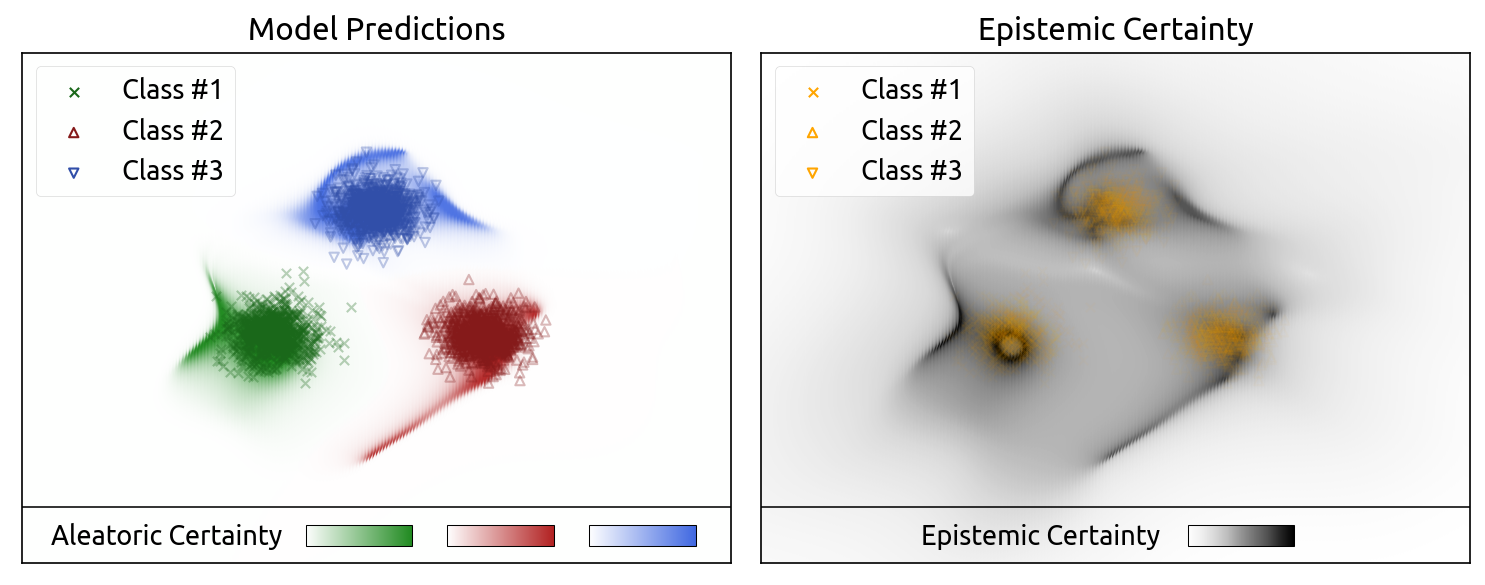
\includegraphics[width=1\textwidth]{sections/007_iclr2022/resources/appendix/toy-900-900-900.png}
    \end{subfigure}%
    %\begin{subfigure}[t]{.75\textwidth}
    %    \centering
    %    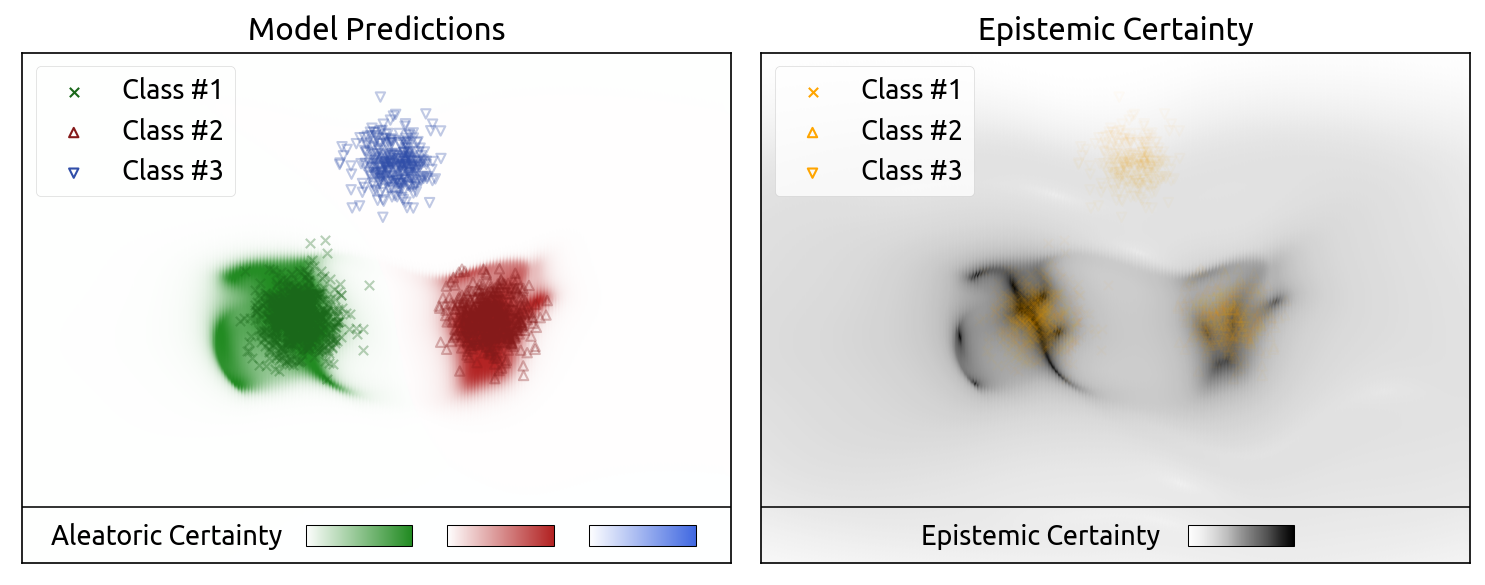
\includegraphics[width=1\textwidth]{sections/007_iclr2022/resources/appendix/toy-900-600-300.png}
    %\end{subfigure}%
\end{figure}

\begin{figure}[ht!]
    \centering
    \caption{Visualization of the aleatoric and epistemic uncertainty on a 2D toy dataset with 3 classes with $900$ training samples for class 1 (green), $600$ training samples for class 2 (red) and $300$ training samples for class 2 (blue).}
    \label{fig:toy-visualization-2-app}
    \begin{subfigure}[t]{.75\textwidth}
        \centering
        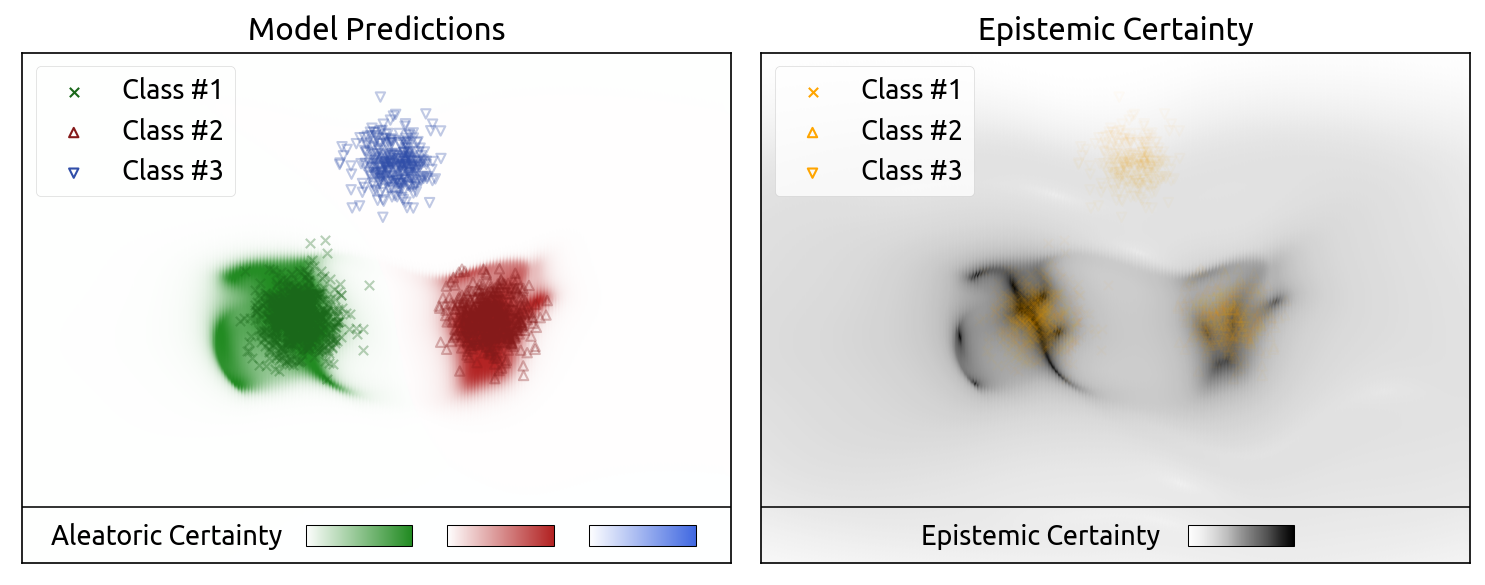
\includegraphics[width=1\textwidth]{sections/007_iclr2022/resources/appendix/toy-900-600-300.png}
    \end{subfigure}%
\end{figure}

\subsection{Latent Space Visualizations}

We propose additional visualizations of the latent space for MNIST with t-SNE \citep{tsne} with different perplexities (see Fig.~\ref{fig:latent-space}). For all perplexities, we clearly observe ten green clusters corresponding to the ten classes for MNIST. The KNMIST (OOD) samples in red can easily be separated from the MNIST (ID) samples in green. As desired, \NatPNacro{} assigns higher log-probabilities used in evidence computation to ID samples from MNIST.

\begin{figure}[ht!]
    \centering
    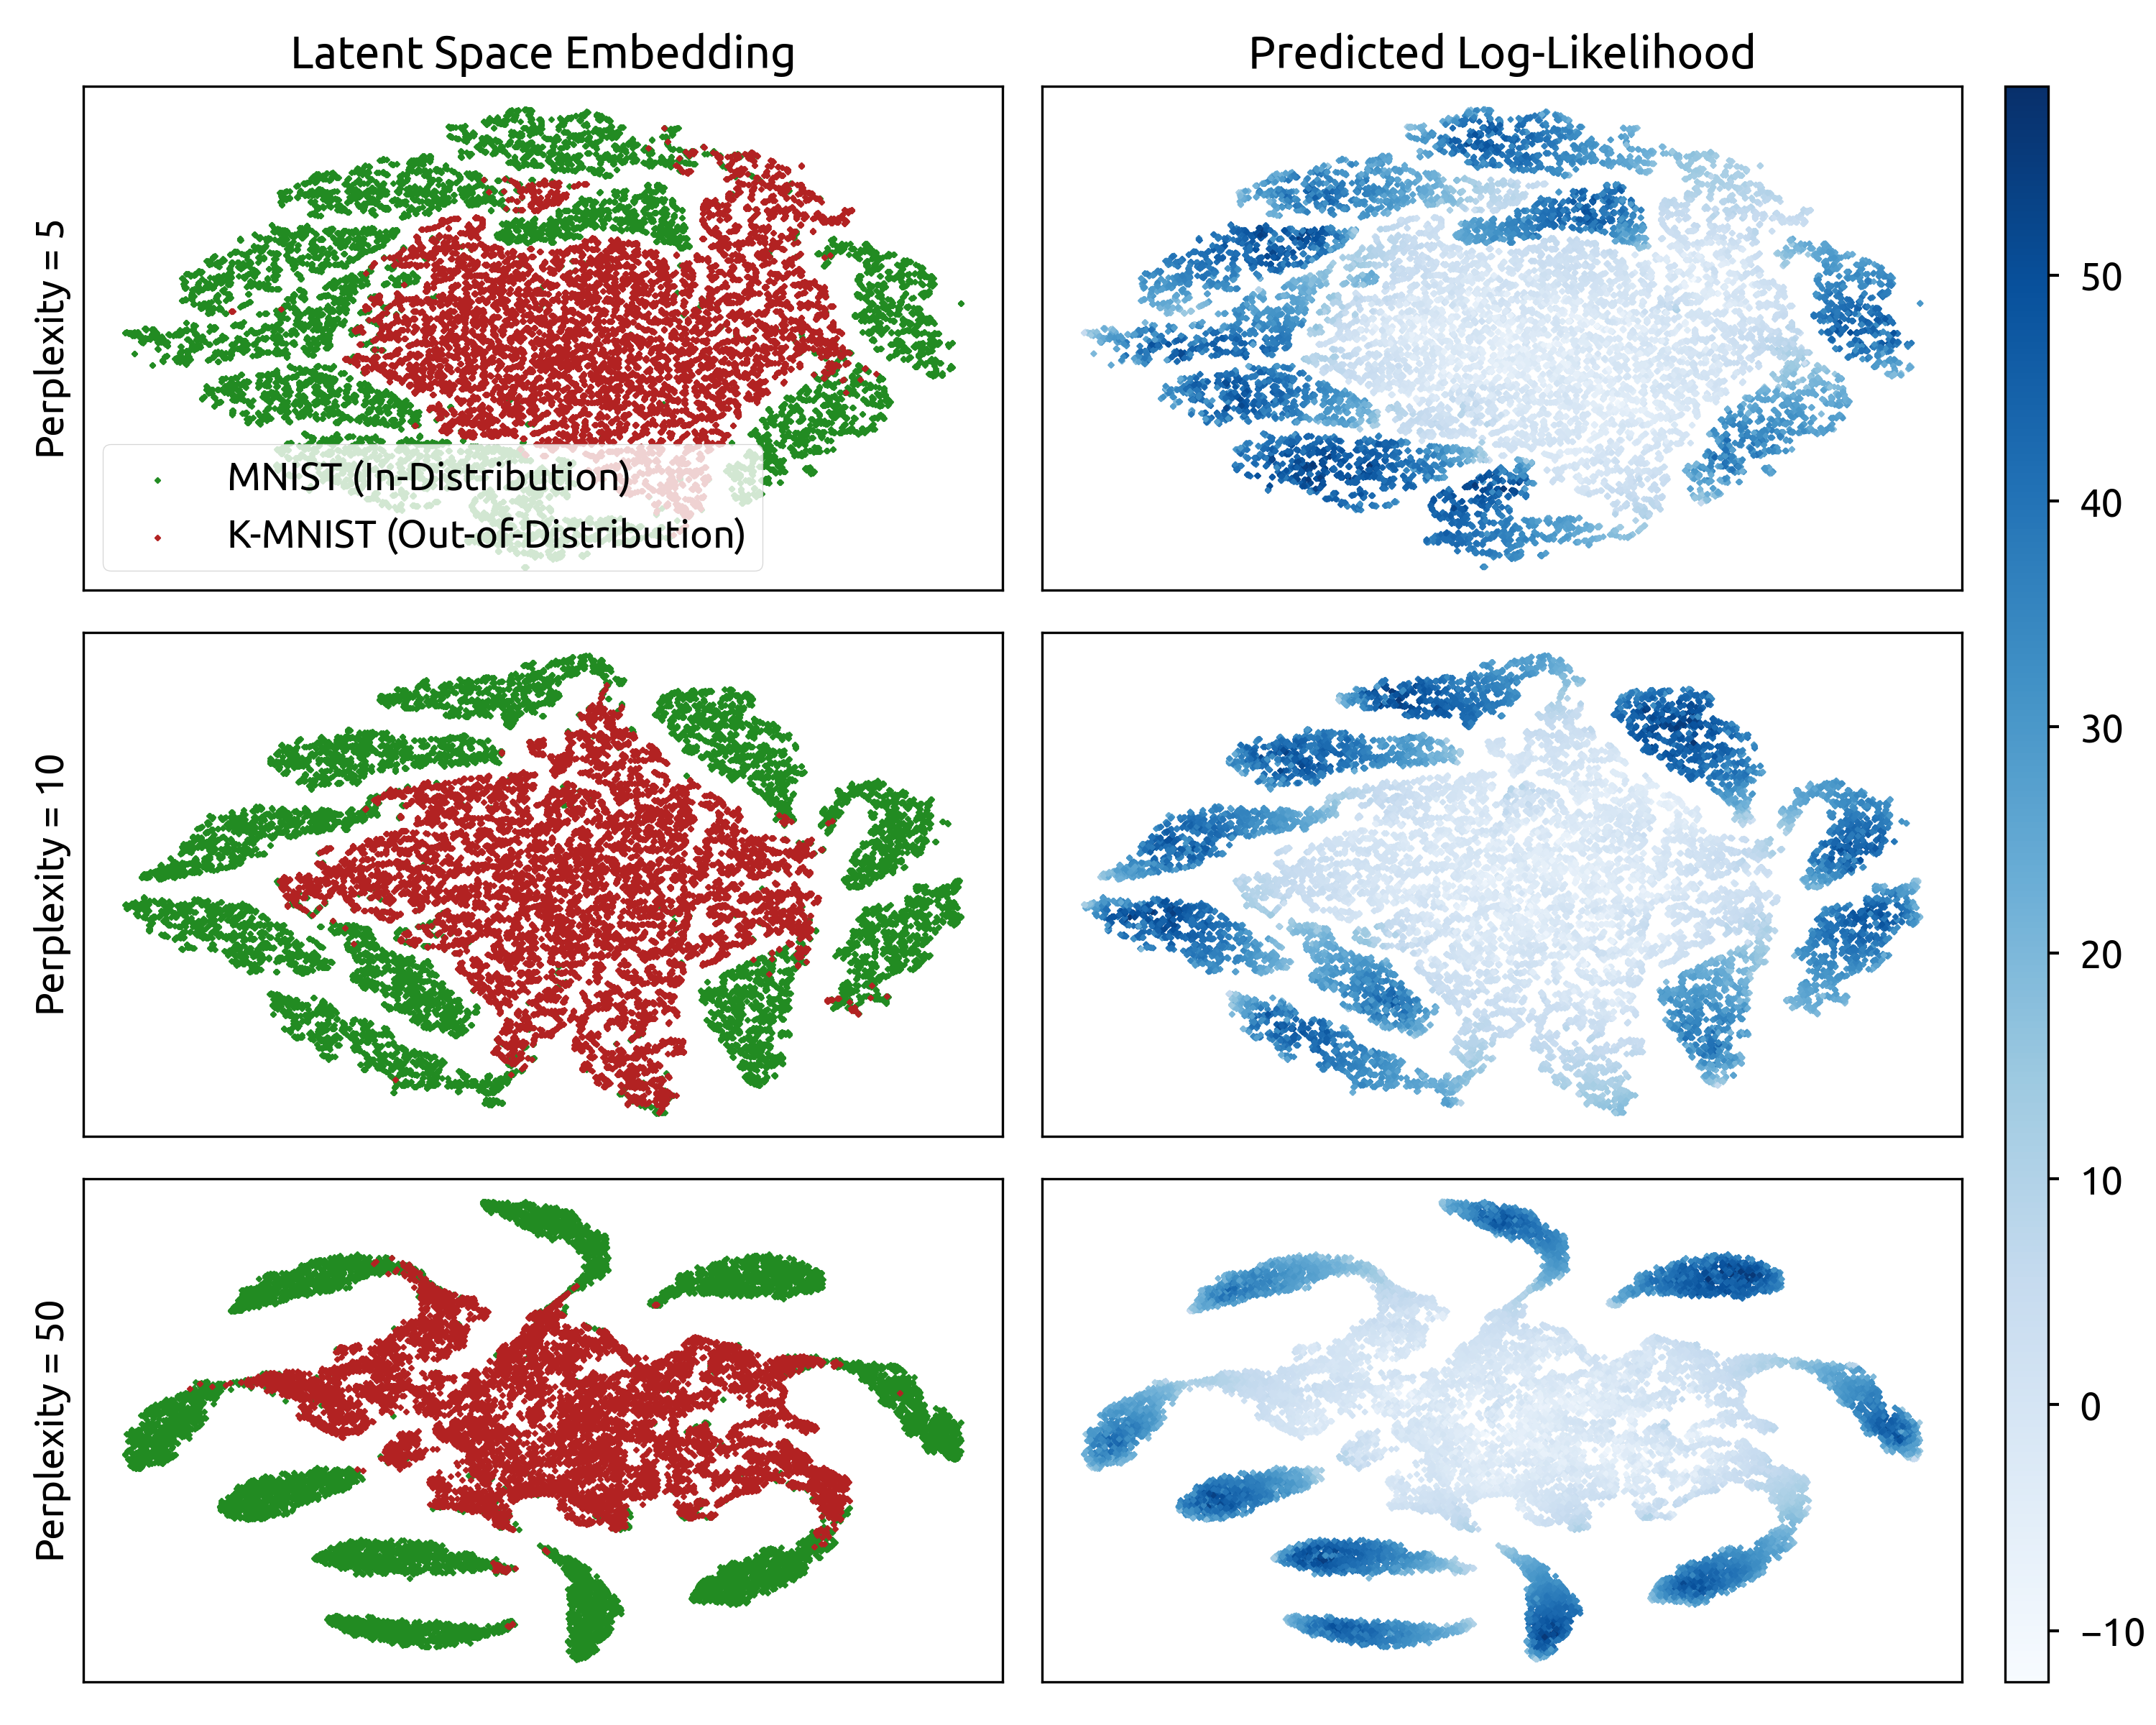
\includegraphics[width=0.6 \textwidth]{sections/007_iclr2022/resources/appendix/embedding-new.png}
    \caption{t-SNE visualization of the latent space of \NatPNacro{} on MNIST (ID) vs KMNIST (OOD). On the left, The ID data (MNIST in green) can easily be distinguished from the OOD data (KMNIST in red). On the right, \NatPNacro{} correctly assigns higher likelihood to ID data.}
    \label{fig:latent-space}
\end{figure}

\subsection{Histogram of Uncertainty Estimates}

We visualize the histogram distribution of the entropy of the posterior distribution accounting for predictive uncertainty for ID (MNIST/NYU) and OOD (KNMIST and Fashion-MNIST/LSUN classroom and LSUN church + KITTI) (see Fig.~\ref{fig:entropy-histograms}). We clearly observe lower predictive entropy for ID data than for OOD data for both MNIST and NYU datasets. On one hand, the entropy clearly differentiates between ID data (MNIST) and any other OOD datasets (KMNIST, Fashion MNIST, OODom) for classification. We intuitively explain this clear distinction since the samples from the OOD datasets are irrelevant for the digit classification task. On the other hand, the entropy is still a good indicator of ID (NYU) and OOD datasets (LSUN classroom and LSUN church + KITTI) for regression although the distinction between ID and OOD datasets is less strong compared to MNIST. We intuitively explain this behavior since the task of depth estimation is still relevant to LSUN classroom and LSUN church + KITTI.

\begin{figure}[ht!]
    \centering
    \caption{Histogram of the entropy of the posterior distribution accounting for the predictive uncertainty of \NatPNacro{} on MNIST (ID) vs KMNIST, Fashion-MNIST, Out-Of-Domain (OOD) and NYU (ID) vs LSUN classroom and LSUN church + KITTI (OOD). In both cases, low entropy is a good indicator of in-distribution data.}
    \label{fig:entropy-histograms}
    \begin{subfigure}[t]{.5\textwidth}
        \centering
    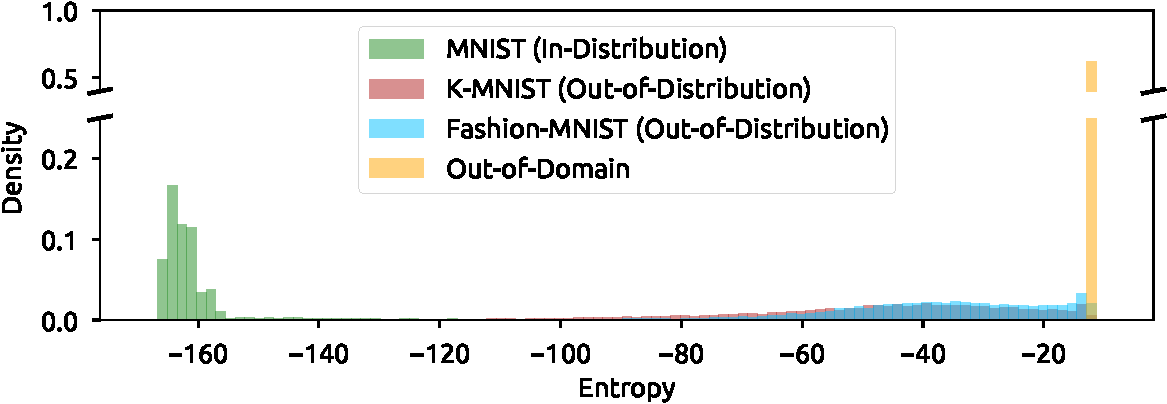
\includegraphics[width=1.\textwidth]{sections/007_iclr2022/resources/appendix/mnist-entropy-new.pdf}
    \end{subfigure}%
    \begin{subfigure}[t]{.5\textwidth}
        \centering
    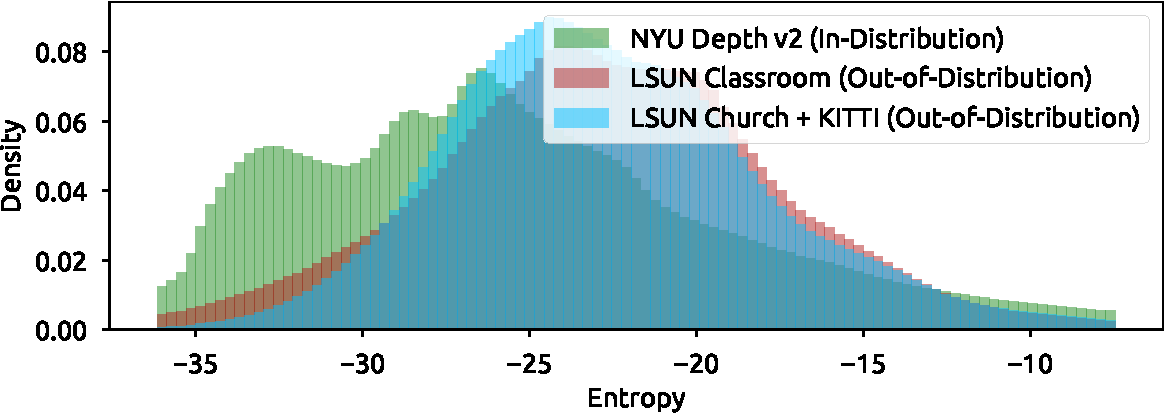
\includegraphics[width=1.0\textwidth]{sections/007_iclr2022/resources/appendix/nyu-entropy-new-ii.pdf}
    \end{subfigure}%
\end{figure}

\subsection{Uncertainty Visualization on NYU Depth v2 Dataset}

We visualize the prediction and the predictive uncertainty per pixel for the NYU Depth v2 dataset (see Fig.~\ref{fig:nyu-uncertainty-visualization}). We observe accurate target predictions compared to the ground truth depth of the images. Further \NatPNacro{} assigns higher uncertainty for pixels close to object edges, which is reasonable since the depth abruptly change at these locations.

\begin{figure}[ht!]
    \centering
    \caption{Visualization of the predicted depth and predictive uncertainty estimates of \NatPNacro{} per pixel on the NYU Depth v2 dataset. \NatPNacro{} predicts accurate depth uncertainty and reasonably assigns higher uncertainty to object edges.}
    \label{fig:nyu-uncertainty-visualization}
    \begin{subfigure}[t]{.5\textwidth}
        \centering
        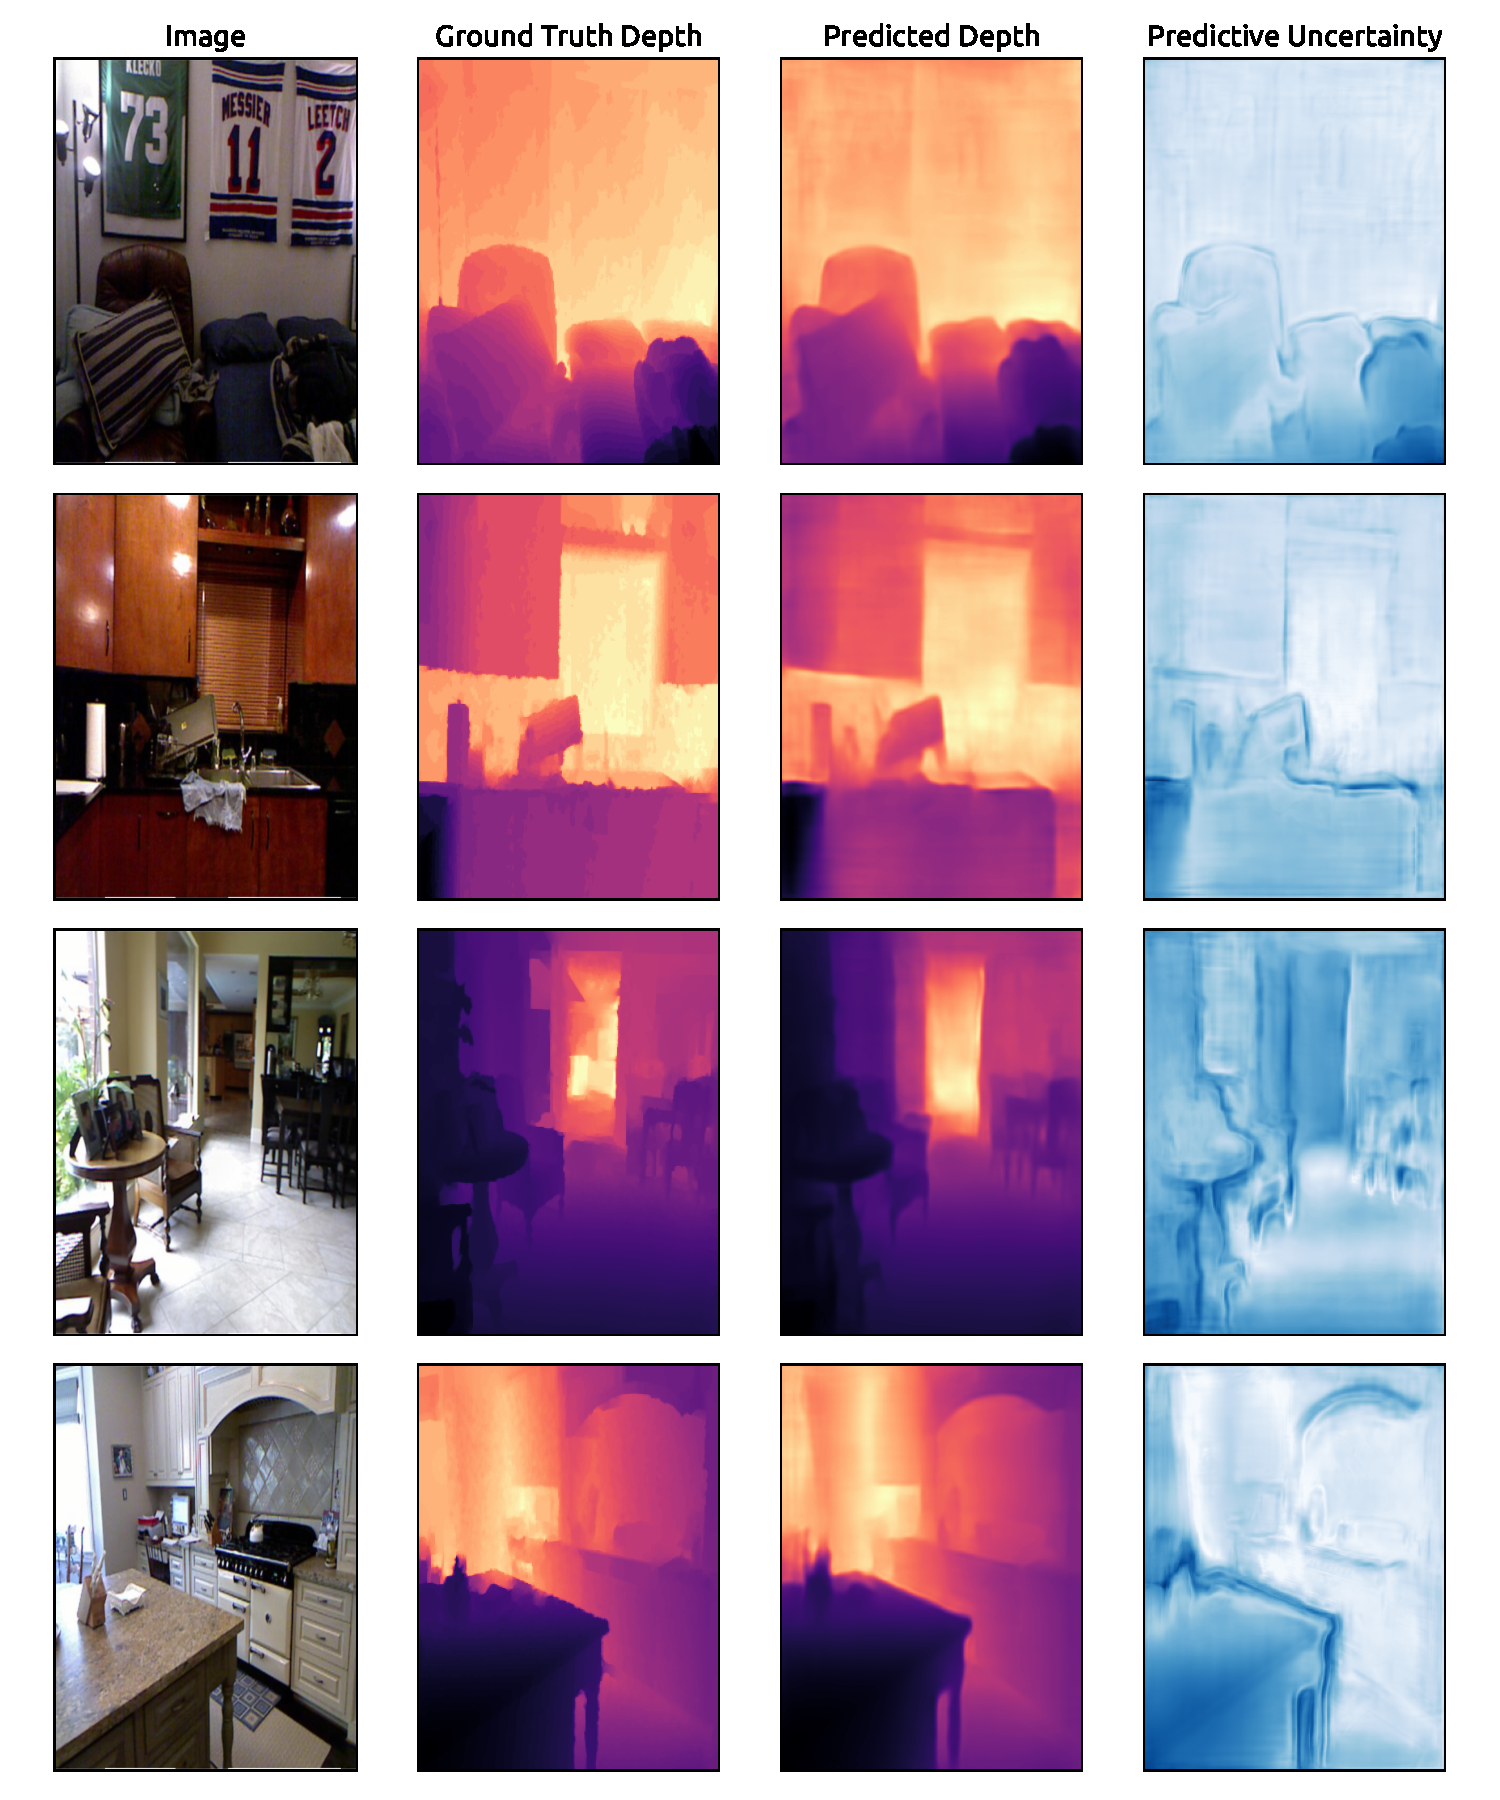
\includegraphics[width=1\textwidth]{sections/007_iclr2022/resources/appendix/nyu-42-new-ii.pdf}
    \end{subfigure}%
    \begin{subfigure}[t]{.5\textwidth}
        \centering
        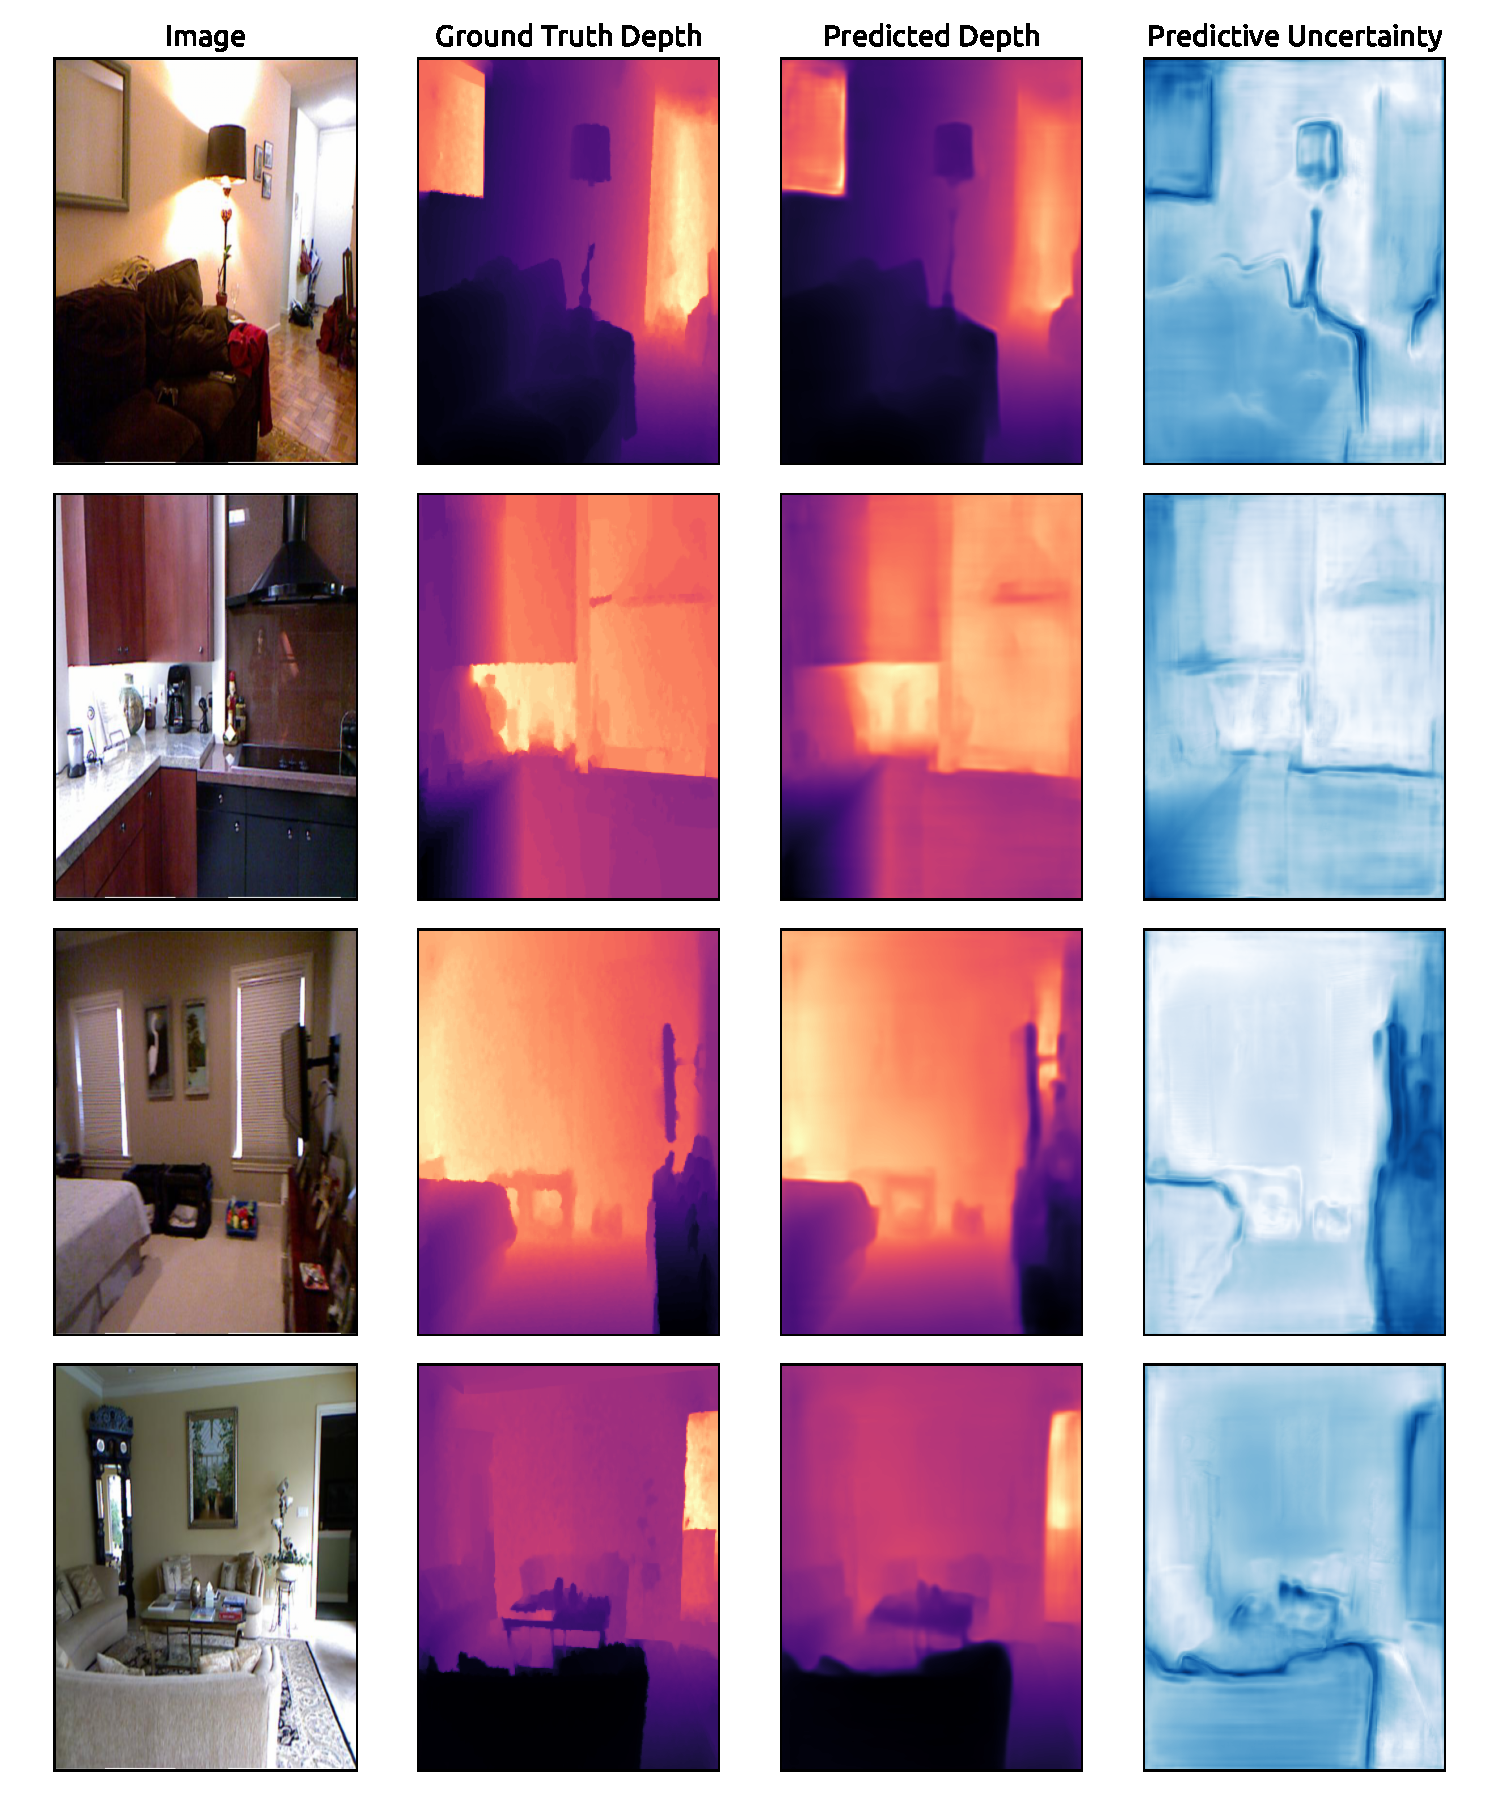
\includegraphics[width=1\textwidth]{sections/007_iclr2022/resources/appendix/nyu-84-new-ii.pdf}
    \end{subfigure}%
\end{figure}


\subsection{Hyper-Parameter Study}
\label{sec:ablation-study_007}

As a ablation study, we also report the results of the grid search on the latent dimension, normalizing flow types and number of normalizing flow layers for MNIST, CIFAR-10 and Bike Sharing datasets in Tab.~\ref{tab:ablation-mnist}, \ref{tab:ablation-cifar10}, \ref{tab:ablation-bikesharing-normal}, \ref{tab:ablation-bikesharing-poisson}. While most models converge to fairly good uncertainty estimates, we notice that 16 layers of simple radial flows on latent spaces of 16 dimensions were achieving very good results in practice. 

Changing the flow type or the number of normalizing flow layers does not lead to strong variations of the results except for Bike sharing with Poisson target distributions. In this case, more complex MAF normalizing flows improve \NatPNacro{} performance. 

The latent dimension appears to be a more important choice for the model convergence. As an example, a higher latent dimension of $16$ or $32$ leads to significantly better performances than a latent dimension of $4$ on MNIST, CIFAR10 and Bike Sharing datasets. We hypothesize that too low latent dimensions are less able to encode the necessary information for the prediction task, leading to worse target errors.

Further, we compare three different variants of the certainty budget $N_H$ used in the evidence computation $\evidence\dataix = N_H\prob(\z\dataix \condition \bm{\omega})$: a constant unit budget (i.e. $N_H=1$ (I)) corresponding to a fixed budget regardless of the number of training data and the latent dimension, a budget equals to the number of training data (i.e. $N_H=N$ (II)) similarly to \citet{charpentier2020}, or a budget which scales exponentially with the number of latent dimensions (e.g. $N_\latentdim$ equal to $e^{\frac{1}{2}\latentdim}$ (III), $e^{\latentdim}$ (IV) or $e^{\log(\sqrt{4\pi})\latentdim}$ (V)). We observe that scaling the budget w.r.t. the latent space dimension ($H$-budget) is more stable in practice than constant budget ($1$-budget) and budget related to the number of training data ($N$-budget) (see. Tab.~\ref{tab:ablation-mnist},\ref{tab:ablation-cifar10},\ref{tab:ablation-bikesharing-normal},\ref{tab:ablation-bikesharing-poisson}). In aprticular, the $H$-budgets achieve more  better results on higher latent dimensions and performance on par with the other certainty budget scheme otherwise. The intuition is that due to the curse of dimensionality, the expected value of a probability density function $\expectation_{\z}[\prob(\z)]$ tends to decrease exponentially fast. For example, we have $\expectation_{\z}[\prob(\z)] = \frac{1}{(\sqrt{4\pi})^H}$ when $\z \sim \DNormal(\bm{0, \bm{1}})$ in a $H$-dimensional space. Increasing the certainty budget $N_H$ exponentially w.r.t. to the dimension $H$ avoids numerical issues by allocating close to $0$ evidence to latent representations. In our experiments, we use a grid search in different exponential scaling $N_\latentdim$ equal to $e^{\frac{1}{2}\latentdim}$ (III), $e^{\latentdim}$ (IV),  $e^{\log(\sqrt{4\pi})\latentdim}$ (V).

\subsection{OOD Detection with AUC-ROC Scores}
\label{sec:auroc}

In addition to the AUC-APR scores, we report the OOD detection results for MNIST, CIFAR10 and Bike Sharing datasets in Tab.~\ref{tab:auroc-mnist}, \ref{tab:auroc-cifar10}, \ref{tab:auroc-bikesharing} with AUC-ROC scores. Similarly as with AUC-APR scores, \NatPNacro{} and NatPE achieve very competitive performances compare to the baselines. It particular, they outperform all baselines to detect challenging OODom data.

\begin{table*}[ht]
    \centering
    \caption{MNIST comparison (<latent dim> -- <certainty budget> -- <radial layers>/<MAF layers>). Bold and starred number indicate best score among all models.}
    \label{tab:ablation-mnist}
    \scriptsize
    \resizebox{\textwidth}{!}{
    \begin{tabular}{lcccccccc}
        \toprule
        & \textbf{Accuracy} & \textbf{Brier} & \textbf{K. Alea.} & \textbf{K. Epist.} & \textbf{F. Alea.} & \textbf{F. Epist.} & \textbf{OODom Alea.} & \textbf{OODom Epist.} \\
        \midrule
        \textbf{$H$ = 4, $N_H$ = I, Flow = 8/0} & 61.92 $\pm$ 3.79 & 64.33 $\pm$ 3.98 & 88.70 $\pm$ 1.65 & 87.66 $\pm$ 2.47 & 90.07 $\pm$ 3.43 & 89.52 $\pm$ 2.25 & \textbf{*100.00 $\pm$ 0.00} & \textbf{*100.00 $\pm$ 0.00} \\
        \textbf{$H$ = 4, $N_H$ = I, Flow = 16/0} & 77.46 $\pm$ 6.26 & 59.11 $\pm$ 1.96 & 91.38 $\pm$ 2.50 & 91.48 $\pm$ 0.85 & 92.46 $\pm$ 1.72 & 93.03 $\pm$ 1.60 & 99.91 $\pm$ 0.04 & \textbf{*100.00 $\pm$ 0.00} \\
        \textbf{$H$ = 4, $N_H$ = I, Flow = 0/4} & 75.04 $\pm$ 10.10 & 59.46 $\pm$ 9.92 & 92.36 $\pm$ 3.34 & 92.64 $\pm$ 4.06 & 93.28 $\pm$ 2.66 & 91.90 $\pm$ 4.71 & 99.82 $\pm$ 0.05 & \textbf{*100.00 $\pm$ 0.00} \\
        \textbf{$H$ = 4, $N_H$ = I, Flow = 0/8} & 80.97 $\pm$ 4.29 & 58.35 $\pm$ 1.75 & 91.87 $\pm$ 2.55 & 92.65 $\pm$ 2.52 & 93.58 $\pm$ 2.93 & 96.50 $\pm$ 1.32 & 99.85 $\pm$ 0.04 & \textbf{*100.00 $\pm$ 0.00} \\
        \midrule
        \textbf{$H$ = 4, $N_H$ = II, Flow = 8/0} & 99.33 $\pm$ 0.05 & 3.43 $\pm$ 0.08 & 92.45 $\pm$ 0.33 & 67.84 $\pm$ 2.95 & 96.55 $\pm$ 1.23 & 71.57 $\pm$ 4.00 & \textbf{*100.00 $\pm$ 0.00} & \textbf{*100.00 $\pm$ 0.00} \\
        \textbf{$H$ = 4, $N_H$ = II, Flow = 16/0} & 99.36 $\pm$ 0.03 & 2.72 $\pm$ 0.08 & 94.87 $\pm$ 0.49 & 86.13 $\pm$ 1.47 & 95.03 $\pm$ 0.44 & 88.62 $\pm$ 1.80 & \textbf{*100.00 $\pm$ 0.00} & \textbf{*100.00 $\pm$ 0.00} \\
        \textbf{$H$ = 4, $N_H$ = II, Flow = 0/4} & 98.86 $\pm$ 0.05 & 4.26 $\pm$ 0.90 & 98.93 $\pm$ 0.16 & 98.04 $\pm$ 0.38 & 99.16 $\pm$ 0.23 & 98.52 $\pm$ 0.52 & 99.71 $\pm$ 0.02 & \textbf{*100.00 $\pm$ 0.00} \\
        \textbf{$H$ = 4, $N_H$ = II, Flow = 0/8} & 98.77 $\pm$ 0.15 & 5.44 $\pm$ 1.57 & 98.43 $\pm$ 0.26 & 97.87 $\pm$ 0.40 & 98.85 $\pm$ 0.26 & 98.35 $\pm$ 0.44 & 99.76 $\pm$ 0.03 & \textbf{*100.00 $\pm$ 0.00} \\
        \midrule
        \textbf{$H$ = 4, $N_H$ = III, Flow = 8/0} & 78.14 $\pm$ 5.55 & 48.46 $\pm$ 4.78 & 88.79 $\pm$ 1.05 & 87.28 $\pm$ 1.96 & 90.56 $\pm$ 1.10 & 89.69 $\pm$ 1.88 & \textbf{*100.00 $\pm$ 0.00} & 99.99 $\pm$ 0.01 \\
        \textbf{$H$ = 4, $N_H$ = III, Flow = 16/0} & 79.56 $\pm$ 5.27 & 41.44 $\pm$ 4.86 & 93.92 $\pm$ 1.25 & 93.99 $\pm$ 0.39 & 95.61 $\pm$ 0.88 & 95.64 $\pm$ 0.58 & 99.92 $\pm$ 0.07 & \textbf{*100.00 $\pm$ 0.00} \\
        \textbf{$H$ = 4, $N_H$ = III, Flow = 0/4} & 76.08 $\pm$ 7.67 & 58.56 $\pm$ 11.60 & 93.72 $\pm$ 3.51 & 94.58 $\pm$ 2.66 & 94.34 $\pm$ 3.39 & 96.60 $\pm$ 1.86 & 99.86 $\pm$ 0.05 & \textbf{*100.00 $\pm$ 0.00} \\
        \textbf{$H$ = 4, $N_H$ = III, Flow = 0/8} & 79.91 $\pm$ 10.84 & 50.78 $\pm$ 10.99 & 94.91 $\pm$ 2.23 & 96.44 $\pm$ 1.49 & 95.97 $\pm$ 1.37 & 98.35 $\pm$ 0.54 & 99.78 $\pm$ 0.07 & \textbf{*100.00 $\pm$ 0.00} \\
        \midrule
        \textbf{$H$ = 4, $N_H$ = IV, Flow = 8/0} & 85.31 $\pm$ 3.89 & 34.01 $\pm$ 5.20 & 89.65 $\pm$ 1.24 & 86.81 $\pm$ 1.36 & 92.78 $\pm$ 0.40 & 86.93 $\pm$ 2.47 & \textbf{*100.00 $\pm$ 0.00} & 99.99 $\pm$ 0.00 \\
        \textbf{$H$ = 4, $N_H$ = IV, Flow = 16/0} & 89.36 $\pm$ 0.15 & 26.48 $\pm$ 2.64 & 94.56 $\pm$ 0.65 & 93.48 $\pm$ 0.88 & 96.03 $\pm$ 1.01 & 94.74 $\pm$ 1.26 & 99.98 $\pm$ 0.02 & \textbf{*100.00 $\pm$ 0.00} \\
        \textbf{$H$ = 4, $N_H$ = IV, Flow = 0/4} & 91.64 $\pm$ 6.70 & 22.61 $\pm$ 13.67 & 96.63 $\pm$ 1.92 & 93.07 $\pm$ 1.49 & 98.43 $\pm$ 0.52 & 94.55 $\pm$ 2.01 & 99.81 $\pm$ 0.06 & \textbf{*100.00 $\pm$ 0.00} \\
        \textbf{$H$ = 4, $N_H$ = IV, Flow = 0/8} & 98.14 $\pm$ 0.46 & 12.73 $\pm$ 5.11 & 98.68 $\pm$ 0.25 & 97.61 $\pm$ 0.64 & 98.93 $\pm$ 0.20 & 97.73 $\pm$ 0.63 & 99.78 $\pm$ 0.05 & \textbf{*100.00 $\pm$ 0.00} \\
        \midrule
        \textbf{$H$ = 4, $N_H$ = V, Flow = 8/0} & 93.59 $\pm$ 2.32 & 20.40 $\pm$ 3.68 & 92.06 $\pm$ 1.39 & 87.15 $\pm$ 2.25 & 93.55 $\pm$ 1.03 & 87.11 $\pm$ 2.97 & \textbf{*100.00 $\pm$ 0.00} & 99.99 $\pm$ 0.00 \\
        \textbf{$H$ = 4, $N_H$ = V, Flow = 16/0} & 97.19 $\pm$ 1.97 & 14.66 $\pm$ 3.13 & 94.67 $\pm$ 1.45 & 92.82 $\pm$ 1.04 & 95.80 $\pm$ 1.17 & 95.27 $\pm$ 0.70 & \textbf{*100.00 $\pm$ 0.00} & \textbf{*100.00 $\pm$ 0.00} \\
        \textbf{$H$ = 4, $N_H$ = V, Flow = 0/4} & 96.69 $\pm$ 1.56 & 16.51 $\pm$ 6.21 & 97.78 $\pm$ 0.63 & 94.58 $\pm$ 1.06 & 96.95 $\pm$ 1.76 & 92.94 $\pm$ 1.74 & 99.80 $\pm$ 0.03 & \textbf{*100.00 $\pm$ 0.00} \\
        \textbf{$H$ = 4, $N_H$ = V, Flow = 0/8} & 98.34 $\pm$ 0.19 & 6.72 $\pm$ 1.54 & 98.85 $\pm$ 0.15 & 98.02 $\pm$ 0.49 & 99.08 $\pm$ 0.08 & 98.41 $\pm$ 0.34 & 99.69 $\pm$ 0.04 & \textbf{*100.00 $\pm$ 0.00} \\
        \midrule
        \midrule
        \textbf{$H$ = 16, $N_H$ = I, Flow = 8/0} & 99.45 $\pm$ 0.04 & 1.49 $\pm$ 0.11 & 97.75 $\pm$ 0.32 & 89.16 $\pm$ 0.34 & 98.13 $\pm$ 0.27 & 89.16 $\pm$ 0.41 & \textbf{*100.00 $\pm$ 0.00} & \textbf{*100.00 $\pm$ 0.00} \\
        \textbf{$H$ = 16, $N_H$ = I, Flow = 16/0} & 99.48 $\pm$ 0.01 & 1.41 $\pm$ 0.07 & \textbf{*99.32 $\pm$ 0.11} & 99.34 $\pm$ 0.05 & \textbf{*99.52 $\pm$ 0.07} & \textbf{*99.59 $\pm$ 0.05} & \textbf{*100.00 $\pm$ 0.00} & \textbf{*100.00 $\pm$ 0.00} \\
        \textbf{$H$ = 16, $N_H$ = I, Flow = 0/4} & 99.18 $\pm$ 0.05 & 1.83 $\pm$ 0.08 & 98.78 $\pm$ 0.11 & 97.92 $\pm$ 0.15 & 99.39 $\pm$ 0.07 & 98.32 $\pm$ 0.51 & 99.93 $\pm$ 0.02 & \textbf{*100.00 $\pm$ 0.00} \\
        \textbf{$H$ = 16, $N_H$ = I, Flow = 0/8} & 99.13 $\pm$ 0.06 & 1.97 $\pm$ 0.09 & 98.97 $\pm$ 0.04 & 98.33 $\pm$ 0.07 & \textbf{*99.52 $\pm$ 0.04} & 99.28 $\pm$ 0.09 & 99.88 $\pm$ 0.02 & \textbf{*100.00 $\pm$ 0.00} \\
        \midrule
        \textbf{$H$ = 16, $N_H$ = II, Flow = 8/0} & 99.42 $\pm$ 0.02 & 1.42 $\pm$ 0.10 & 96.62 $\pm$ 0.37 & 82.95 $\pm$ 1.46 & 97.34 $\pm$ 0.59 & 82.85 $\pm$ 1.37 & \textbf{*100.00 $\pm$ 0.00} & \textbf{*100.00 $\pm$ 0.00} \\
        \textbf{$H$ = 16, $N_H$ = II, Flow = 16/0} & 99.39 $\pm$ 0.02 & 1.52 $\pm$ 0.23 & 98.19 $\pm$ 0.38 & 95.92 $\pm$ 1.30 & 98.48 $\pm$ 0.37 & 96.20 $\pm$ 1.30 & \textbf{*100.00 $\pm$ 0.00} & \textbf{*100.00 $\pm$ 0.00} \\
        \textbf{$H$ = 16, $N_H$ = II, Flow = 0/4} & 99.24 $\pm$ 0.04 & 1.74 $\pm$ 0.08 & 98.65 $\pm$ 0.12 & 97.49 $\pm$ 0.20 & 99.29 $\pm$ 0.09 & 98.62 $\pm$ 0.20 & 99.94 $\pm$ 0.02 & \textbf{*100.00 $\pm$ 0.00} \\
        \textbf{$H$ = 16, $N_H$ = II, Flow = 0/8} & 99.26 $\pm$ 0.04 & 1.73 $\pm$ 0.09 & 98.89 $\pm$ 0.06 & 98.09 $\pm$ 0.12 & 99.33 $\pm$ 0.11 & 98.73 $\pm$ 0.27 & 99.95 $\pm$ 0.01 & \textbf{*100.00 $\pm$ 0.00} \\
        \midrule
        \textbf{$H$ = 16, $N_H$ = III, Flow = 8/0} & 99.47 $\pm$ 0.02 & 1.90 $\pm$ 0.50 & 95.08 $\pm$ 1.14 & 83.27 $\pm$ 0.43 & 96.03 $\pm$ 1.33 & 82.95 $\pm$ 0.30 & \textbf{*100.00 $\pm$ 0.00} & \textbf{*100.00 $\pm$ 0.00} \\
        \textbf{$H$ = 16, $N_H$ = III, Flow = 16/0} & 99.47 $\pm$ 0.02 & \textbf{*1.09 $\pm$ 0.03} & 99.20 $\pm$ 0.20 & \textbf{*99.39 $\pm$ 0.08} & 99.16 $\pm$ 0.28 & 99.54 $\pm$ 0.09 & 99.99 $\pm$ 0.01 & \textbf{*100.00 $\pm$ 0.00} \\
        \textbf{$H$ = 16, $N_H$ = III, Flow = 0/4} & 99.25 $\pm$ 0.03 & 1.65 $\pm$ 0.07 & 98.72 $\pm$ 0.07 & 97.95 $\pm$ 0.15 & 99.44 $\pm$ 0.04 & 98.96 $\pm$ 0.17 & 99.95 $\pm$ 0.01 & \textbf{*100.00 $\pm$ 0.00} \\
        \textbf{$H$ = 16, $N_H$ = III, Flow = 0/8} & 99.26 $\pm$ 0.05 & 1.78 $\pm$ 0.07 & 98.89 $\pm$ 0.08 & 98.24 $\pm$ 0.20 & 99.23 $\pm$ 0.28 & 98.70 $\pm$ 0.37 & 99.95 $\pm$ 0.01 & \textbf{*100.00 $\pm$ 0.00} \\
        \midrule
        \textbf{$H$ = 16, $N_H$ = IV, Flow = 8/0} & 99.33 $\pm$ 0.04 & 1.58 $\pm$ 0.03 & 97.08 $\pm$ 0.35 & 77.40 $\pm$ 1.79 & 98.15 $\pm$ 0.61 & 77.46 $\pm$ 1.82 & \textbf{*100.00 $\pm$ 0.00} & \textbf{*100.00 $\pm$ 0.00} \\
        \textbf{$H$ = 16, $N_H$ = IV, Flow = 16/0} & 99.37 $\pm$ 0.03 & 1.47 $\pm$ 0.11 & 97.52 $\pm$ 0.50 & 93.53 $\pm$ 0.89 & 98.04 $\pm$ 0.55 & 94.28 $\pm$ 0.60 & \textbf{*100.00 $\pm$ 0.00} & \textbf{*100.00 $\pm$ 0.00} \\
        \textbf{$H$ = 16, $N_H$ = IV, Flow = 0/4} & 99.23 $\pm$ 0.06 & 1.74 $\pm$ 0.10 & 98.64 $\pm$ 0.06 & 97.00 $\pm$ 0.38 & 99.31 $\pm$ 0.07 & 98.24 $\pm$ 0.35 & 99.93 $\pm$ 0.02 & \textbf{*100.00 $\pm$ 0.00} \\
        \textbf{$H$ = 16, $N_H$ = IV, Flow = 0/8} & 99.17 $\pm$ 0.03 & 1.83 $\pm$ 0.04 & 98.54 $\pm$ 0.10 & 97.43 $\pm$ 0.23 & 99.15 $\pm$ 0.15 & 98.28 $\pm$ 0.34 & 99.93 $\pm$ 0.01 & \textbf{*100.00 $\pm$ 0.00} \\
        \midrule
        \textbf{$H$ = 16, $N_H$ = V, Flow = 8/0} & 99.36 $\pm$ 0.03 & 1.46 $\pm$ 0.02 & 97.60 $\pm$ 0.63 & 72.45 $\pm$ 3.67 & 98.25 $\pm$ 0.83 & 72.69 $\pm$ 3.58 & \textbf{*100.00 $\pm$ 0.00} & \textbf{*100.00 $\pm$ 0.00} \\
        \textbf{$H$ = 16, $N_H$ = V, Flow = 16/0} & 99.38 $\pm$ 0.02 & 1.58 $\pm$ 0.12 & 96.17 $\pm$ 0.61 & 90.44 $\pm$ 1.80 & 96.80 $\pm$ 0.33 & 91.12 $\pm$ 1.87 & \textbf{*100.00 $\pm$ 0.00} & \textbf{*100.00 $\pm$ 0.00} \\
        \textbf{$H$ = 16, $N_H$ = V, Flow = 0/4} & 99.15 $\pm$ 0.04 & 1.89 $\pm$ 0.08 & 98.57 $\pm$ 0.13 & 96.06 $\pm$ 0.34 & 99.08 $\pm$ 0.11 & 97.79 $\pm$ 0.42 & 99.91 $\pm$ 0.01 & \textbf{*100.00 $\pm$ 0.00} \\
        \textbf{$H$ = 16, $N_H$ = V, Flow = 0/8} & 99.23 $\pm$ 0.04 & 1.98 $\pm$ 0.08 & 98.53 $\pm$ 0.04 & 97.03 $\pm$ 0.19 & 98.94 $\pm$ 0.13 & 97.83 $\pm$ 0.20 & 99.90 $\pm$ 0.01 & \textbf{*100.00 $\pm$ 0.00} \\
        \midrule
        \midrule
        \textbf{$H$ = 32, $N_H$ = I, Flow = 8/0} & \textbf{*99.49 $\pm$ 0.03} & 2.28 $\pm$ 0.89 & 92.36 $\pm$ 1.75 & 76.18 $\pm$ 2.10 & 93.90 $\pm$ 1.59 & 76.38 $\pm$ 2.11 & \textbf{*100.00 $\pm$ 0.00} & \textbf{*100.00 $\pm$ 0.00} \\
        \textbf{$H$ = 32, $N_H$ = I, Flow = 16/0} & 99.47 $\pm$ 0.01 & 1.47 $\pm$ 0.26 & 96.20 $\pm$ 0.25 & 95.95 $\pm$ 1.21 & 95.96 $\pm$ 0.77 & 95.97 $\pm$ 1.14 & \textbf{*100.00 $\pm$ 0.00} & \textbf{*100.00 $\pm$ 0.00} \\
        \textbf{$H$ = 32, $N_H$ = I, Flow = 0/4} & 99.29 $\pm$ 0.02 & 1.42 $\pm$ 0.04 & 99.02 $\pm$ 0.05 & 98.14 $\pm$ 0.16 & 99.46 $\pm$ 0.02 & 98.57 $\pm$ 0.11 & 99.95 $\pm$ 0.01 & \textbf{*100.00 $\pm$ 0.00} \\
        \textbf{$H$ = 32, $N_H$ = I, Flow = 0/8} & 99.27 $\pm$ 0.04 & 1.45 $\pm$ 0.06 & 98.95 $\pm$ 0.08 & 98.52 $\pm$ 0.08 & 99.35 $\pm$ 0.06 & 98.80 $\pm$ 0.04 & 99.99 $\pm$ 0.00 & \textbf{*100.00 $\pm$ 0.00} \\
        \midrule
        \textbf{$H$ = 32, $N_H$ = II, Flow = 8/0} & 99.44 $\pm$ 0.05 & 1.29 $\pm$ 0.18 & 96.03 $\pm$ 1.88 & 73.89 $\pm$ 2.45 & 96.83 $\pm$ 1.13 & 73.98 $\pm$ 2.41 & \textbf{*100.00 $\pm$ 0.00} & \textbf{*100.00 $\pm$ 0.00} \\
        \textbf{$H$ = 32, $N_H$ = II, Flow = 16/0} & 99.46 $\pm$ 0.05 & 1.94 $\pm$ 0.79 & 96.57 $\pm$ 1.17 & 94.13 $\pm$ 1.47 & 97.82 $\pm$ 0.84 & 94.69 $\pm$ 1.39 & \textbf{*100.00 $\pm$ 0.00} & \textbf{*100.00 $\pm$ 0.00} \\
        \textbf{$H$ = 32, $N_H$ = II, Flow = 0/4} & 99.26 $\pm$ 0.01 & 1.48 $\pm$ 0.02 & 98.90 $\pm$ 0.05 & 97.98 $\pm$ 0.06 & 99.29 $\pm$ 0.05 & 98.44 $\pm$ 0.09 & 99.94 $\pm$ 0.01 & \textbf{*100.00 $\pm$ 0.00} \\
        \textbf{$H$ = 32, $N_H$ = II, Flow = 0/8} & 99.30 $\pm$ 0.06 & 1.39 $\pm$ 0.09 & 98.89 $\pm$ 0.07 & 98.14 $\pm$ 0.14 & 99.45 $\pm$ 0.06 & 98.64 $\pm$ 0.13 & 99.98 $\pm$ 0.01 & \textbf{*100.00 $\pm$ 0.00} \\
        \midrule
        \textbf{$H$ = 32, $N_H$ = III, Flow = 8/0} & \textbf{*99.49 $\pm$ 0.01} & 1.20 $\pm$ 0.10 & 97.91 $\pm$ 0.79 & 73.77 $\pm$ 3.06 & 98.73 $\pm$ 0.57 & 73.79 $\pm$ 2.97 & \textbf{*100.00 $\pm$ 0.00} & \textbf{*100.00 $\pm$ 0.00} \\
        \textbf{$H$ = 32, $N_H$ = III, Flow = 16/0} & 99.44 $\pm$ 0.02 & 1.90 $\pm$ 0.69 & 96.16 $\pm$ 1.53 & 90.95 $\pm$ 1.20 & 97.42 $\pm$ 1.12 & 91.46 $\pm$ 1.24 & \textbf{*100.00 $\pm$ 0.00} & \textbf{*100.00 $\pm$ 0.00} \\
        \textbf{$H$ = 32, $N_H$ = III, Flow = 0/4} & 99.31 $\pm$ 0.02 & 1.38 $\pm$ 0.03 & 98.89 $\pm$ 0.10 & 97.73 $\pm$ 0.06 & 99.29 $\pm$ 0.11 & 98.41 $\pm$ 0.08 & 99.97 $\pm$ 0.01 & \textbf{*100.00 $\pm$ 0.00} \\
        \textbf{$H$ = 32, $N_H$ = III, Flow = 0/8} & 99.28 $\pm$ 0.04 & 1.33 $\pm$ 0.05 & 98.80 $\pm$ 0.09 & 98.16 $\pm$ 0.05 & 99.27 $\pm$ 0.08 & 98.52 $\pm$ 0.13 & 99.98 $\pm$ 0.01 & \textbf{*100.00 $\pm$ 0.00} \\
        \midrule
        \textbf{$H$ = 32, $N_H$ = IV, Flow = 8/0} & 99.36 $\pm$ 0.03 & 1.47 $\pm$ 0.05 & 97.97 $\pm$ 0.39 & 71.87 $\pm$ 1.31 & 99.00 $\pm$ 0.10 & 72.28 $\pm$ 1.30 & \textbf{*100.00 $\pm$ 0.00} & \textbf{*100.00 $\pm$ 0.00} \\
        \textbf{$H$ = 32, $N_H$ = IV, Flow = 16/0} & 99.38 $\pm$ 0.02 & 2.41 $\pm$ 0.66 & 95.45 $\pm$ 1.73 & 83.06 $\pm$ 1.62 & 96.91 $\pm$ 1.24 & 83.48 $\pm$ 1.65 & \textbf{*100.00 $\pm$ 0.00} & \textbf{*100.00 $\pm$ 0.00} \\
        \textbf{$H$ = 32, $N_H$ = IV, Flow = 0/4} & 99.22 $\pm$ 0.03 & 1.50 $\pm$ 0.09 & 98.77 $\pm$ 0.08 & 97.49 $\pm$ 0.11 & 99.27 $\pm$ 0.05 & 98.33 $\pm$ 0.09 & 99.97 $\pm$ 0.01 & \textbf{*100.00 $\pm$ 0.00} \\
        \textbf{$H$ = 32, $N_H$ = IV, Flow = 0/8} & 99.25 $\pm$ 0.04 & 1.34 $\pm$ 0.07 & 98.62 $\pm$ 0.09 & 97.70 $\pm$ 0.15 & 99.24 $\pm$ 0.06 & 98.09 $\pm$ 0.34 & 99.99 $\pm$ 0.00 & \textbf{*100.00 $\pm$ 0.00} \\
        \midrule
        \textbf{$H$ = 32, $N_H$ = V, Flow = 8/0} & 99.35 $\pm$ 0.02 & 1.43 $\pm$ 0.08 & 98.43 $\pm$ 0.29 & 64.15 $\pm$ 3.79 & 99.22 $\pm$ 0.16 & 64.37 $\pm$ 3.84 & \textbf{*100.00 $\pm$ 0.00} & \textbf{*100.00 $\pm$ 0.00} \\
        \textbf{$H$ = 32, $N_H$ = V, Flow = 16/0} & 99.33 $\pm$ 0.03 & 1.76 $\pm$ 0.33 & 97.41 $\pm$ 0.93 & 84.15 $\pm$ 1.84 & 98.26 $\pm$ 0.60 & 85.01 $\pm$ 2.01 & \textbf{*100.00 $\pm$ 0.00} & \textbf{*100.00 $\pm$ 0.00} \\
        \textbf{$H$ = 32, $N_H$ = V, Flow = 0/4} & 99.18 $\pm$ 0.05 & 1.58 $\pm$ 0.08 & 98.61 $\pm$ 0.09 & 96.71 $\pm$ 0.24 & 99.11 $\pm$ 0.07 & 97.34 $\pm$ 0.17 & 99.94 $\pm$ 0.01 & \textbf{*100.00 $\pm$ 0.00} \\
        \textbf{$H$ = 32, $N_H$ = V, Flow = 0/8} & 99.19 $\pm$ 0.03 & 1.58 $\pm$ 0.06 & 98.58 $\pm$ 0.10 & 96.98 $\pm$ 0.15 & 99.19 $\pm$ 0.08 & 96.99 $\pm$ 0.28 & 99.99 $\pm$ 0.00 & \textbf{*100.00 $\pm$ 0.00} \\
        \bottomrule
    \end{tabular}
    }
\end{table*}

% \begin{table*}[ht]
%     \centering
%     \scriptsize
%     \resizebox{0.95 \textwidth}{!}{
%     \begin{tabular}{lcccccccc}
%         \toprule
%         & \textbf{Accuracy} & \textbf{Brier} & \textbf{K. Alea.} & \textbf{K. Epist.} & \textbf{F. Alea.} & \textbf{F. Epist.} & \textbf{OODom Alea.} & \textbf{OODom Epist.} \\
%         \midrule
%         \textbf{\oursacro{} (4 -- 8/0)} & 83.28 $\pm$ 2.08 & 41.21 $\pm$ 2.73 & 91.09 $\pm$ 0.62 & 85.02 $\pm$ 0.97 & 91.76 $\pm$ 1.36 & 84.27 $\pm$ 0.65 & \textbf{*100.00 $\pm$ 0.00} & \textbf{*100.00 $\pm$ 0.00} \\
%         \textbf{\oursacro{} (4 -- 16/0)} & 83.46 $\pm$ 2.37 & 36.60 $\pm$ 2.70 & 95.74 $\pm$ 0.35 & 96.20 $\pm$ 0.45 & 97.41 $\pm$ 0.55 & 97.04 $\pm$ 0.36 & \textbf{*100.00 $\pm$ 0.00} & \textbf{*100.00 $\pm$ 0.00} \\
%         \textbf{\oursacro{} (4 -- 0/4)} & 97.40 $\pm$ 0.78 & 17.82 $\pm$ 6.11 & 98.69 $\pm$ 0.21 & 96.71 $\pm$ 0.81 & 99.43 $\pm$ 0.12 & 98.41 $\pm$ 0.78 & 99.80 $\pm$ 0.04 & \textbf{*100.00 $\pm$ 0.00} \\
%         \textbf{\oursacro{} (4 -- 0/8)} & 96.09 $\pm$ 1.52 & 25.57 $\pm$ 8.28 & 98.14 $\pm$ 0.36 & 97.04 $\pm$ 1.01 & 99.19 $\pm$ 0.16 & 98.72 $\pm$ 0.59 & 99.86 $\pm$ 0.03 & \textbf{*100.00 $\pm$ 0.00} \\
%         \textbf{\oursacro{} (4 -- 0/16)} & 98.30 $\pm$ 0.19 & 8.10 $\pm$ 0.81 & \textbf{*99.04 $\pm$ 0.19} & 98.32 $\pm$ 0.49 & \textbf{*99.47 $\pm$ 0.06} & \textbf{*99.35 $\pm$ 0.16} & 99.78 $\pm$ 0.04 & \textbf{*100.00 $\pm$ 0.00} \\
%         \midrule
%         \textbf{\oursacro{} (16 -- 8/0)} & 99.34 $\pm$ 0.02 & 1.57 $\pm$ 0.16 & 96.82 $\pm$ 0.52 & 80.57 $\pm$ 1.25 & 96.98 $\pm$ 0.66 & 78.75 $\pm$ 2.06 & \textbf{*100.00 $\pm$ 0.00} & \textbf{*100.00 $\pm$ 0.00} \\
%         \textbf{\oursacro{} (16 -- 16/0)} & \textbf{*99.35 $\pm$ 0.03} & \textbf{*1.38 $\pm$ 0.06} & 98.66 $\pm$ 0.20 & \textbf{*98.52 $\pm$ 0.67} & 99.27 $\pm$ 0.12 & 99.08 $\pm$ 0.42 & 99.96 $\pm$ 0.01 & \textbf{*100.00 $\pm$ 0.00} \\
%         \textbf{\oursacro{} (16 -- 0/4)} & 99.23 $\pm$ 0.04 & 1.89 $\pm$ 0.10 & 98.49 $\pm$ 0.08 & 95.34 $\pm$ 0.84 & 99.14 $\pm$ 0.11 & 96.24 $\pm$ 1.19 & 99.95 $\pm$ 0.01 & \textbf{*100.00 $\pm$ 0.00} \\
%         \textbf{\oursacro{} (16 -- 0/8)} & 99.24 $\pm$ 0.03 & 1.95 $\pm$ 0.13 & 98.64 $\pm$ 0.11 & 96.57 $\pm$ 0.26 & 99.17 $\pm$ 0.13 & 97.84 $\pm$ 0.51 & 99.94 $\pm$ 0.01 & \textbf{*100.00 $\pm$ 0.00} \\
%         \textbf{\oursacro{} (16 -- 0/16)} & 99.20 $\pm$ 0.04 & 1.99 $\pm$ 0.10 & 98.63 $\pm$ 0.07 & 97.47 $\pm$ 0.17 & 99.21 $\pm$ 0.10 & 98.51 $\pm$ 0.36 & 99.93 $\pm$ 0.02 & \textbf{*100.00 $\pm$ 0.00} \\
%         \midrule
%         \textbf{\oursacro{} (32 -- 8/0)} & 99.33 $\pm$ 0.02 & 1.56 $\pm$ 0.06 & 96.12 $\pm$ 0.42 & 73.55 $\pm$ 1.40 & 97.64 $\pm$ 0.72 & 73.24 $\pm$ 1.64 & \textbf{*100.00 $\pm$ 0.00} & \textbf{*100.00 $\pm$ 0.00} \\
%         \textbf{\oursacro{} (32 -- 16/0)} & \textbf{*99.35 $\pm$ 0.03} & 3.73 $\pm$ 2.08 & 96.03 $\pm$ 1.61 & 88.85 $\pm$ 3.60 & 96.83 $\pm$ 1.46 & 89.15 $\pm$ 3.66 & \textbf{*100.00 $\pm$ 0.00} & \textbf{*100.00 $\pm$ 0.00} \\
%         \textbf{\oursacro{} (32 -- 0/4)} & 99.16 $\pm$ 0.04 & 1.64 $\pm$ 0.09 & 98.48 $\pm$ 0.10 & 96.92 $\pm$ 0.20 & 99.01 $\pm$ 0.09 & 98.11 $\pm$ 0.14 & 99.96 $\pm$ 0.01 & \textbf{*100.00 $\pm$ 0.00} \\
%         \textbf{\oursacro{} (32 -- 0/8)} & 99.17 $\pm$ 0.03 & 1.66 $\pm$ 0.03 & 98.47 $\pm$ 0.04 & 97.26 $\pm$ 0.26 & 99.15 $\pm$ 0.07 & 98.25 $\pm$ 0.31 & 99.97 $\pm$ 0.01 & \textbf{*100.00 $\pm$ 0.00} \\
%         \textbf{\oursacro{} (32 -- 0/16)} & 99.16 $\pm$ 0.02 & 1.66 $\pm$ 0.08 & 98.35 $\pm$ 0.09 & 97.60 $\pm$ 0.07 & 98.88 $\pm$ 0.15 & 97.98 $\pm$ 0.30 & 99.99 $\pm$ 0.00 & \textbf{*100.00 $\pm$ 0.00} \\
%         \bottomrule
%     \end{tabular}
%     }
%     \caption{MNIST Comparison (<latent dim> -- <radial layers>/<MAF layers>). Bold and starred number indicate best score among all models.}
%     \label{tab:ablation-mnist}
% \end{table*}

% \begin{table*}[ht]
%     \centering
%     \scriptsize
%     \resizebox{0.95 \textwidth}{!}{
%     \begin{tabular}{lcccccccc}
%         \toprule
%         & \textbf{Accuracy} & \textbf{Brier} & \textbf{K. Alea.} & \textbf{K. Epist.} & \textbf{F. Alea.} & \textbf{F. Epist.} & \textbf{OODom Alea.} & \textbf{OODom Epist.} \\
%         \midrule
%         \textbf{\oursacro{}} ($1$-budget) & \textbf{*99.51 $\pm$ 0.01} & \textbf{*1.22 $\pm$ 0.10} & 99.23 $\pm$ 0.13 & 99.41 $\pm$ 0.02 & 99.24 $\pm$ 0.08 & 99.38 $\pm$ 0.04 & \textbf{*100.00 $\pm$ 0.00} & \textbf{*100.00 $\pm$ 0.00} \\
%         \textbf{\oursacro{}} ($N$-budget) & 99.40 $\pm$ 0.03 & 1.24 $\pm$ 0.05 & \textbf{*99.42 $\pm$ 0.03} & \textbf{*99.44 $\pm$ 0.02} & \textbf{*99.44 $\pm$ 0.06} & \textbf{*99.53 $\pm$ 0.05} & 99.99 $\pm$ 0.00 & \textbf{*100.00 $\pm$ 0.00} \\
%         \textbf{\oursacro{}} ($H$-budget) & 99.35 $\pm$ 0.03 & 1.38 $\pm$ 0.06 & 98.66 $\pm$ 0.20 & 98.52 $\pm$ 0.67 & 99.27 $\pm$ 0.12 & 99.08 $\pm$ 0.42 & 99.96 $\pm$ 0.01 & \textbf{*100.00 $\pm$ 0.00} \\
%         %\textbf{\oursacro{} ($N_H = $ new)} & 99.33 $\pm$ 0.03 & 1.79 $\pm$ 0.27 & 97.54 $\pm$ 0.31 & 93.14 $\pm$ 1.30 & 98.55 $\pm$ 0.33 & 93.93 $\pm$ 1.27 & \textbf{*100.00 $\pm$ 0.00} & \textbf{*100.00 $\pm$ 0.00} \\
%         \bottomrule
%     \end{tabular}
%     }
%     \caption{MNIST Comparison $N_H$ Scaling. Bold and starred number indicate best score among all models.}
%     \label{tab:ablation-mnist-log-scale}
% \end{table*}

\begin{table*}[ht]
    \centering
    \caption{CIFAR10 comparison (<latent dim> -- <certainty budget> -- <radial layers>/<MAF layers>). Bold and starred number indicate best score among all models.}
    \label{tab:ablation-cifar10}
    \scriptsize
    \resizebox{\textwidth}{!}{
    \begin{tabular}{lcccccccc}
        \toprule
        & \textbf{Accuracy} & \textbf{Brier} & \textbf{SVHN Alea.} & \textbf{SVHN Epist.} & \textbf{CelebA Alea.} & \textbf{CelebA Epist.} & \textbf{OODom Alea.} & \textbf{OODom Epist.} \\
        \midrule
        \textbf{$H$ = 4, $N_H$ = I, Flow = 8/0} & 42.73 $\pm$ 6.40 & 81.56 $\pm$ 2.72 & 67.03 $\pm$ 3.15 & 49.84 $\pm$ 6.09 & 56.86 $\pm$ 2.13 & 39.01 $\pm$ 7.65 & 95.33 $\pm$ 4.48 & 97.68 $\pm$ 2.32 \\
        \textbf{$H$ = 4, $N_H$ = I, Flow = 16/0} & 46.39 $\pm$ 6.64 & 77.73 $\pm$ 3.57 & 66.43 $\pm$ 2.39 & 46.63 $\pm$ 5.92 & 68.22 $\pm$ 3.82 & 41.98 $\pm$ 6.52 & 98.93 $\pm$ 0.85 & 99.61 $\pm$ 0.39 \\
        \textbf{$H$ = 4, $N_H$ = I, Flow = 0/4} & 53.79 $\pm$ 2.51 & 80.83 $\pm$ 4.54 & 59.77 $\pm$ 5.82 & 35.96 $\pm$ 2.59 & 64.95 $\pm$ 1.92 & 48.27 $\pm$ 5.85 & 97.76 $\pm$ 1.90 & 99.86 $\pm$ 0.07 \\
        \textbf{$H$ = 4, $N_H$ = I, Flow = 0/8} & 51.11 $\pm$ 3.67 & 79.13 $\pm$ 2.10 & 58.22 $\pm$ 4.19 & 33.22 $\pm$ 8.03 & 63.97 $\pm$ 3.12 & 42.75 $\pm$ 9.47 & 84.62 $\pm$ 10.88 & 88.24 $\pm$ 11.76 \\
        \midrule
        \textbf{$H$ = 4, $N_H$ = II, Flow = 8/0} & 88.02 $\pm$ 0.12 & 22.61 $\pm$ 0.18 & 75.40 $\pm$ 2.82 & 40.98 $\pm$ 3.98 & 62.73 $\pm$ 6.72 & 35.68 $\pm$ 3.66 & 82.17 $\pm$ 3.49 & 60.66 $\pm$ 7.27 \\
        \textbf{$H$ = 4, $N_H$ = II, Flow = 16/0} & 87.80 $\pm$ 0.09 & 22.43 $\pm$ 0.33 & 78.00 $\pm$ 1.68 & 60.02 $\pm$ 2.96 & 63.55 $\pm$ 2.08 & 46.15 $\pm$ 4.20 & 88.55 $\pm$ 3.72 & 88.82 $\pm$ 2.85 \\
        \textbf{$H$ = 4, $N_H$ = II, Flow = 0/4} & 87.10 $\pm$ 0.10 & 22.42 $\pm$ 0.16 & 83.35 $\pm$ 0.72 & 67.89 $\pm$ 4.11 & 75.76 $\pm$ 1.33 & 63.04 $\pm$ 4.04 & 89.20 $\pm$ 3.60 & 91.43 $\pm$ 3.81 \\
        \textbf{$H$ = 4, $N_H$ = II, Flow = 0/8} & 86.28 $\pm$ 0.74 & 24.15 $\pm$ 1.52 & 83.69 $\pm$ 0.48 & 67.20 $\pm$ 3.22 & 75.30 $\pm$ 1.66 & 63.56 $\pm$ 5.25 & 80.92 $\pm$ 8.99 & 83.04 $\pm$ 7.45 \\
        \midrule
        \textbf{$H$ = 4, $N_H$ = III, Flow = 8/0} & 68.54 $\pm$ 4.06 & 64.35 $\pm$ 3.30 & 71.61 $\pm$ 2.06 & 57.05 $\pm$ 5.90 & 70.14 $\pm$ 2.66 & 51.87 $\pm$ 3.56 & 93.39 $\pm$ 6.00 & 95.61 $\pm$ 3.82 \\
        \textbf{$H$ = 4, $N_H$ = III, Flow = 16/0} & 69.41 $\pm$ 4.00 & 59.98 $\pm$ 4.79 & 74.52 $\pm$ 1.11 & 52.59 $\pm$ 6.96 & 73.48 $\pm$ 2.43 & 51.59 $\pm$ 7.09 & 93.43 $\pm$ 3.42 & 93.45 $\pm$ 4.86 \\
        \textbf{$H$ = 4, $N_H$ = III, Flow = 0/4} & 64.80 $\pm$ 4.59 & 61.82 $\pm$ 5.62 & 67.99 $\pm$ 3.37 & 37.00 $\pm$ 6.95 & 66.88 $\pm$ 5.61 & 38.00 $\pm$ 10.01 & 99.70 $\pm$ 0.02 & 99.97 $\pm$ 0.02 \\
        \textbf{$H$ = 4, $N_H$ = III, Flow = 0/8} & 61.49 $\pm$ 5.78 & 66.53 $\pm$ 6.29 & 57.58 $\pm$ 5.84 & 34.37 $\pm$ 3.79 & 62.22 $\pm$ 6.68 & 39.86 $\pm$ 9.87 & 94.73 $\pm$ 3.13 & 98.71 $\pm$ 1.02 \\
        \midrule
        \textbf{$H$ = 4, $N_H$ = IV, Flow = 8/0} & 84.45 $\pm$ 0.44 & 38.86 $\pm$ 1.13 & 73.65 $\pm$ 1.66 & 53.64 $\pm$ 1.71 & 71.68 $\pm$ 2.13 & 52.30 $\pm$ 1.49 & 69.65 $\pm$ 5.61 & 66.36 $\pm$ 7.76 \\
        \textbf{$H$ = 4, $N_H$ = IV, Flow = 16/0} & 83.16 $\pm$ 0.83 & 35.51 $\pm$ 1.55 & 80.65 $\pm$ 2.67 & 59.70 $\pm$ 3.43 & 76.69 $\pm$ 3.23 & 50.09 $\pm$ 2.76 & 80.24 $\pm$ 7.59 & 83.05 $\pm$ 5.77 \\
        \textbf{$H$ = 4, $N_H$ = IV, Flow = 0/4} & 72.13 $\pm$ 2.90 & 48.67 $\pm$ 3.63 & 72.17 $\pm$ 1.95 & 27.43 $\pm$ 3.60 & 71.77 $\pm$ 2.24 & 27.09 $\pm$ 2.25 & 99.22 $\pm$ 0.53 & 99.85 $\pm$ 0.09 \\
        \textbf{$H$ = 4, $N_H$ = IV, Flow = 0/8} & 72.34 $\pm$ 1.84 & 51.55 $\pm$ 3.08 & 68.02 $\pm$ 3.39 & 28.48 $\pm$ 2.16 & 69.02 $\pm$ 2.91 & 32.72 $\pm$ 4.89 & 99.13 $\pm$ 0.44 & 98.91 $\pm$ 0.68 \\
        \midrule
        \textbf{$H$ = 4, $N_H$ = V, Flow = 8/0} & 86.32 $\pm$ 0.64 & 32.24 $\pm$ 1.38 & 73.15 $\pm$ 4.29 & 50.79 $\pm$ 3.87 & 66.37 $\pm$ 6.81 & 47.11 $\pm$ 7.35 & 73.58 $\pm$ 7.20 & 63.29 $\pm$ 5.99 \\
        \textbf{$H$ = 4, $N_H$ = V, Flow = 16/0} & 86.18 $\pm$ 0.39 & 27.92 $\pm$ 0.56 & 79.67 $\pm$ 2.46 & 56.96 $\pm$ 4.80 & 74.68 $\pm$ 2.69 & 45.29 $\pm$ 5.32 & 77.59 $\pm$ 10.23 & 80.75 $\pm$ 8.14 \\
        \textbf{$H$ = 4, $N_H$ = V, Flow = 0/4} & 80.39 $\pm$ 0.94 & 37.33 $\pm$ 2.23 & 77.81 $\pm$ 2.52 & 31.59 $\pm$ 3.34 & 74.14 $\pm$ 1.57 & 31.93 $\pm$ 3.75 & 93.63 $\pm$ 5.76 & 93.85 $\pm$ 5.61 \\
        \textbf{$H$ = 4, $N_H$ = V, Flow = 0/8} & 77.84 $\pm$ 0.71 & 42.01 $\pm$ 1.03 & 75.27 $\pm$ 2.23 & 40.87 $\pm$ 6.42 & 73.46 $\pm$ 1.81 & 33.18 $\pm$ 5.09 & 98.59 $\pm$ 0.72 & 99.08 $\pm$ 0.61 \\
        \midrule
        \midrule
        \textbf{$H$ = 16, $N_H$ = I, Flow = 8/0} & 82.83 $\pm$ 0.84 & 30.89 $\pm$ 1.71 & 81.35 $\pm$ 0.60 & 65.51 $\pm$ 2.65 & 75.48 $\pm$ 1.65 & 61.89 $\pm$ 3.89 & 99.73 $\pm$ 0.24 & 99.82 $\pm$ 0.18 \\
        \textbf{$H$ = 16, $N_H$ = I, Flow = 16/0} & 84.83 $\pm$ 0.60 & 26.24 $\pm$ 1.06 & 82.39 $\pm$ 1.11 & 75.54 $\pm$ 2.52 & 75.30 $\pm$ 0.72 & 69.12 $\pm$ 2.15 & 99.90 $\pm$ 0.06 & 99.96 $\pm$ 0.04 \\
        \textbf{$H$ = 16, $N_H$ = I, Flow = 0/4} & 83.71 $\pm$ 1.37 & 27.35 $\pm$ 2.34 & 81.38 $\pm$ 0.94 & 56.29 $\pm$ 4.77 & 75.88 $\pm$ 0.51 & 51.73 $\pm$ 4.32 & 99.17 $\pm$ 0.65 & 99.92 $\pm$ 0.07 \\
        \textbf{$H$ = 16, $N_H$ = I, Flow = 0/8} & 84.13 $\pm$ 0.53 & 27.02 $\pm$ 1.02 & 80.24 $\pm$ 1.88 & 67.03 $\pm$ 2.59 & 74.59 $\pm$ 0.68 & 58.67 $\pm$ 8.57 & 99.93 $\pm$ 0.01 & \textbf{*100.00 $\pm$ 0.00} \\
        \midrule
        \textbf{$H$ = 16, $N_H$ = II, Flow = 8/0} & 86.82 $\pm$ 0.46 & 22.45 $\pm$ 0.88 & 83.73 $\pm$ 1.26 & 56.60 $\pm$ 3.15 & 76.98 $\pm$ 1.67 & 63.55 $\pm$ 2.26 & 85.41 $\pm$ 11.05 & 87.59 $\pm$ 7.40 \\
        \textbf{$H$ = 16, $N_H$ = II, Flow = 16/0} & 86.40 $\pm$ 0.46 & 23.06 $\pm$ 0.82 & 83.60 $\pm$ 0.96 & 74.04 $\pm$ 2.78 & 76.87 $\pm$ 0.92 & 74.00 $\pm$ 1.92 & 82.09 $\pm$ 10.05 & 92.84 $\pm$ 3.70 \\
        \textbf{$H$ = 16, $N_H$ = II, Flow = 0/4} & 88.02 $\pm$ 0.12 & 19.83 $\pm$ 0.21 & 81.19 $\pm$ 0.77 & 72.46 $\pm$ 1.88 & 74.19 $\pm$ 1.54 & 65.32 $\pm$ 2.02 & 99.14 $\pm$ 0.59 & 99.90 $\pm$ 0.07 \\
        \textbf{$H$ = 16, $N_H$ = II, Flow = 0/8} & 87.73 $\pm$ 0.11 & 19.97 $\pm$ 0.33 & 83.29 $\pm$ 0.70 & 71.93 $\pm$ 1.90 & 74.14 $\pm$ 2.13 & 63.20 $\pm$ 3.16 & 99.94 $\pm$ 0.01 & \textbf{*100.00 $\pm$ 0.00} \\
        \midrule
        \textbf{$H$ = 16, $N_H$ = III, Flow = 8/0} & 86.54 $\pm$ 0.55 & 23.44 $\pm$ 1.10 & 80.97 $\pm$ 1.57 & 59.46 $\pm$ 1.33 & 73.31 $\pm$ 2.36 & 58.10 $\pm$ 3.38 & 93.95 $\pm$ 2.43 & 91.07 $\pm$ 3.26 \\
        \textbf{$H$ = 16, $N_H$ = III, Flow = 16/0} & 86.89 $\pm$ 0.20 & 22.07 $\pm$ 0.41 & 83.11 $\pm$ 0.43 & 72.37 $\pm$ 1.29 & 75.52 $\pm$ 0.83 & 72.66 $\pm$ 3.46 & 96.20 $\pm$ 2.51 & 98.21 $\pm$ 1.06 \\
        \textbf{$H$ = 16, $N_H$ = III, Flow = 0/4} & 88.16 $\pm$ 0.16 & 19.54 $\pm$ 0.22 & 82.50 $\pm$ 1.29 & 62.54 $\pm$ 1.59 & 74.62 $\pm$ 0.98 & 57.76 $\pm$ 2.44 & 99.89 $\pm$ 0.01 & \textbf{*100.00 $\pm$ 0.00} \\
        \textbf{$H$ = 16, $N_H$ = III, Flow = 0/8} & 87.67 $\pm$ 0.17 & 20.23 $\pm$ 0.38 & 84.03 $\pm$ 0.93 & 70.91 $\pm$ 1.97 & 73.43 $\pm$ 1.33 & 61.20 $\pm$ 1.55 & 99.90 $\pm$ 0.03 & 99.99 $\pm$ 0.00 \\
        \midrule
        \textbf{$H$ = 16, $N_H$ = IV, Flow = 8/0} & 87.97 $\pm$ 0.07 & 19.98 $\pm$ 0.17 & \textbf{*84.42 $\pm$ 0.82} & 62.10 $\pm$ 0.56 & 72.25 $\pm$ 1.85 & 65.17 $\pm$ 5.34 & 90.96 $\pm$ 4.50 & 81.63 $\pm$ 9.18 \\
        \textbf{$H$ = 16, $N_H$ = IV, Flow = 16/0} & 87.90 $\pm$ 0.16 & 19.99 $\pm$ 0.46 & 82.29 $\pm$ 1.11 & \textbf{*77.83 $\pm$ 1.22} & 76.01 $\pm$ 1.18 & \textbf{*76.87 $\pm$ 3.38} & 93.67 $\pm$ 3.03 & 94.90 $\pm$ 3.09 \\
        \textbf{$H$ = 16, $N_H$ = IV, Flow = 0/4} & 87.92 $\pm$ 0.22 & 19.93 $\pm$ 0.38 & 82.26 $\pm$ 1.22 & 67.03 $\pm$ 2.75 & 73.28 $\pm$ 1.25 & 63.06 $\pm$ 2.78 & 99.91 $\pm$ 0.02 & \textbf{*100.00 $\pm$ 0.00} \\
        \textbf{$H$ = 16, $N_H$ = IV, Flow = 0/8} & 87.90 $\pm$ 0.19 & 19.70 $\pm$ 0.28 & 81.72 $\pm$ 0.44 & 64.76 $\pm$ 4.18 & 74.90 $\pm$ 0.94 & 66.46 $\pm$ 3.04 & 99.82 $\pm$ 0.12 & 99.99 $\pm$ 0.01 \\
        \midrule
        \textbf{$H$ = 16, $N_H$ = V, Flow = 8/0} & 88.17 $\pm$ 0.17 & 19.78 $\pm$ 0.29 & 83.67 $\pm$ 0.66 & 56.34 $\pm$ 0.85 & 74.32 $\pm$ 2.32 & 62.47 $\pm$ 1.08 & 95.06 $\pm$ 1.51 & 82.09 $\pm$ 6.85 \\
        \textbf{$H$ = 16, $N_H$ = V, Flow = 16/0} & 88.17 $\pm$ 0.16 & 19.81 $\pm$ 0.34 & 81.76 $\pm$ 1.19 & 68.45 $\pm$ 1.60 & 72.98 $\pm$ 1.93 & 71.08 $\pm$ 4.11 & 83.74 $\pm$ 6.25 & 86.85 $\pm$ 3.37 \\
        \textbf{$H$ = 16, $N_H$ = V, Flow = 0/4} & 88.24 $\pm$ 0.12 & 19.30 $\pm$ 0.25 & 83.57 $\pm$ 0.67 & 66.44 $\pm$ 3.12 & 76.16 $\pm$ 1.94 & 63.04 $\pm$ 2.90 & 99.10 $\pm$ 0.84 & 99.97 $\pm$ 0.02 \\
        \textbf{$H$ = 16, $N_H$ = V, Flow = 0/8} & 88.10 $\pm$ 0.20 & 19.32 $\pm$ 0.40 & 81.22 $\pm$ 1.29 & 71.88 $\pm$ 2.05 & 75.42 $\pm$ 0.96 & 66.06 $\pm$ 2.02 & 99.74 $\pm$ 0.18 & 99.99 $\pm$ 0.00 \\
        \midrule
        \midrule
        \textbf{$H$ = 32, $N_H$ = I, Flow = 8/0} & 10.05 $\pm$ 0.28 & 95.02 $\pm$ 0.03 & 27.35 $\pm$ 1.29 & 23.46 $\pm$ 1.45 & 35.30 $\pm$ 1.88 & 34.31 $\pm$ 1.47 & 97.06 $\pm$ 0.64 & \textbf{*100.00 $\pm$ 0.00} \\
        \textbf{$H$ = 32, $N_H$ = I, Flow = 16/0} & 83.94 $\pm$ 0.61 & 27.83 $\pm$ 1.22 & 81.71 $\pm$ 0.62 & 74.15 $\pm$ 2.21 & 75.62 $\pm$ 1.48 & 75.68 $\pm$ 4.15 & 99.94 $\pm$ 0.02 & 99.97 $\pm$ 0.03 \\
        \textbf{$H$ = 32, $N_H$ = I, Flow = 0/4} & 85.30 $\pm$ 0.86 & 24.67 $\pm$ 1.56 & 82.70 $\pm$ 1.54 & 66.68 $\pm$ 2.56 & 76.15 $\pm$ 1.88 & 62.01 $\pm$ 0.96 & 99.93 $\pm$ 0.02 & \textbf{*100.00 $\pm$ 0.00} \\
        \textbf{$H$ = 32, $N_H$ = I, Flow = 0/8} & 85.58 $\pm$ 0.32 & 24.04 $\pm$ 0.73 & 82.77 $\pm$ 1.10 & 57.03 $\pm$ 2.71 & 75.48 $\pm$ 1.25 & 56.44 $\pm$ 1.77 & 99.84 $\pm$ 0.11 & \textbf{*100.00 $\pm$ 0.00} \\
        \midrule
        \textbf{$H$ = 32, $N_H$ = II, Flow = 8/0} & 86.11 $\pm$ 0.41 & 23.61 $\pm$ 0.82 & 83.38 $\pm$ 0.71 & 52.99 $\pm$ 2.55 & 76.14 $\pm$ 1.43 & 60.70 $\pm$ 1.29 & 95.80 $\pm$ 2.55 & 95.44 $\pm$ 2.79 \\
        \textbf{$H$ = 32, $N_H$ = II, Flow = 16/0} & 86.28 $\pm$ 0.31 & 23.11 $\pm$ 0.54 & 83.00 $\pm$ 0.53 & 63.42 $\pm$ 3.35 & 73.87 $\pm$ 1.19 & 72.90 $\pm$ 3.19 & 97.87 $\pm$ 2.04 & 99.92 $\pm$ 0.05 \\
        \textbf{$H$ = 32, $N_H$ = II, Flow = 0/4} & 87.98 $\pm$ 0.12 & 19.62 $\pm$ 0.22 & 82.72 $\pm$ 0.77 & 58.53 $\pm$ 4.37 & 74.45 $\pm$ 1.96 & 57.56 $\pm$ 4.88 & 99.93 $\pm$ 0.04 & \textbf{*100.00 $\pm$ 0.00} \\
        \textbf{$H$ = 32, $N_H$ = II, Flow = 0/8} & 87.41 $\pm$ 0.45 & 20.73 $\pm$ 0.78 & 81.91 $\pm$ 1.56 & 63.56 $\pm$ 2.61 & 75.30 $\pm$ 0.85 & 58.86 $\pm$ 3.76 & 99.97 $\pm$ 0.01 & \textbf{*100.00 $\pm$ 0.00} \\
        \midrule
        \textbf{$H$ = 32, $N_H$ = III, Flow = 8/0} & 86.65 $\pm$ 0.08 & 22.53 $\pm$ 0.18 & 82.38 $\pm$ 0.45 & 51.04 $\pm$ 1.13 & 74.93 $\pm$ 0.97 & 62.11 $\pm$ 1.92 & 95.20 $\pm$ 2.24 & 92.17 $\pm$ 5.43 \\
        \textbf{$H$ = 32, $N_H$ = III, Flow = 16/0} & 85.71 $\pm$ 0.47 & 24.29 $\pm$ 0.88 & 82.65 $\pm$ 0.59 & 66.63 $\pm$ 3.54 & 76.55 $\pm$ 1.22 & 73.27 $\pm$ 1.09 & 98.27 $\pm$ 1.24 & 98.75 $\pm$ 1.14 \\
        \textbf{$H$ = 32, $N_H$ = III, Flow = 0/4} & 88.05 $\pm$ 0.17 & 19.54 $\pm$ 0.34 & 81.85 $\pm$ 0.94 & 63.19 $\pm$ 2.75 & 76.21 $\pm$ 0.84 & 61.44 $\pm$ 4.30 & 99.75 $\pm$ 0.21 & \textbf{*100.00 $\pm$ 0.00} \\
        \textbf{$H$ = 32, $N_H$ = III, Flow = 0/8} & 88.23 $\pm$ 0.37 & 19.48 $\pm$ 0.62 & 84.08 $\pm$ 1.42 & 64.08 $\pm$ 3.71 & \textbf{*78.26 $\pm$ 1.27} & 64.08 $\pm$ 1.55 & \textbf{*99.98 $\pm$ 0.01} & \textbf{*100.00 $\pm$ 0.00} \\
        \midrule
        \textbf{$H$ = 32, $N_H$ = IV, Flow = 8/0} & 88.02 $\pm$ 0.19 & 19.78 $\pm$ 0.32 & 83.24 $\pm$ 0.65 & 50.51 $\pm$ 4.65 & 77.52 $\pm$ 1.20 & 60.08 $\pm$ 2.16 & 95.24 $\pm$ 2.10 & 91.41 $\pm$ 3.61 \\
        \textbf{$H$ = 32, $N_H$ = IV, Flow = 16/0} & 88.29 $\pm$ 0.14 & 19.36 $\pm$ 0.31 & 82.62 $\pm$ 1.72 & 59.43 $\pm$ 5.41 & 73.52 $\pm$ 1.33 & 59.20 $\pm$ 5.22 & 97.56 $\pm$ 1.00 & 99.57 $\pm$ 0.39 \\
        \textbf{$H$ = 32, $N_H$ = IV, Flow = 0/4} & 87.83 $\pm$ 0.14 & 19.92 $\pm$ 0.24 & 83.23 $\pm$ 0.71 & 57.29 $\pm$ 5.16 & 74.99 $\pm$ 1.71 & 65.64 $\pm$ 3.16 & 99.93 $\pm$ 0.04 & \textbf{*100.00 $\pm$ 0.00} \\
        \textbf{$H$ = 32, $N_H$ = IV, Flow = 0/8} & 88.24 $\pm$ 0.28 & \textbf{*19.25 $\pm$ 0.44} & 82.82 $\pm$ 1.17 & 64.69 $\pm$ 2.96 & 73.58 $\pm$ 2.12 & 60.43 $\pm$ 3.12 & 99.27 $\pm$ 0.43 & 99.99 $\pm$ 0.01 \\
        \midrule
        \textbf{$H$ = 32, $N_H$ = V, Flow = 8/0} & 88.25 $\pm$ 0.11 & 19.43 $\pm$ 0.25 & 83.02 $\pm$ 0.60 & 48.85 $\pm$ 3.13 & 73.55 $\pm$ 2.21 & 54.24 $\pm$ 3.53 & 94.02 $\pm$ 2.56 & 83.94 $\pm$ 5.81 \\
        \textbf{$H$ = 32, $N_H$ = V, Flow = 16/0} & 88.30 $\pm$ 0.17 & 19.41 $\pm$ 0.34 & 83.35 $\pm$ 1.37 & 64.63 $\pm$ 3.58 & 75.89 $\pm$ 2.13 & 72.53 $\pm$ 3.19 & 95.68 $\pm$ 0.75 & 95.89 $\pm$ 2.84 \\
        \textbf{$H$ = 32, $N_H$ = V, Flow = 0/4} & \textbf{*88.41 $\pm$ 0.15} & 19.34 $\pm$ 0.26 & 84.03 $\pm$ 0.94 & 59.12 $\pm$ 3.95 & 74.31 $\pm$ 1.96 & 63.33 $\pm$ 1.89 & 99.73 $\pm$ 0.13 & 99.99 $\pm$ 0.00 \\
        \textbf{$H$ = 32, $N_H$ = V, Flow = 0/8} & 88.26 $\pm$ 0.10 & 19.28 $\pm$ 0.10 & 83.68 $\pm$ 0.69 & 60.66 $\pm$ 2.92 & 73.08 $\pm$ 1.57 & 61.10 $\pm$ 5.28 & 99.28 $\pm$ 0.28 & \textbf{*100.00 $\pm$ 0.00} \\
        \bottomrule
    \end{tabular}
    }
\end{table*}

% \begin{table*}[ht]
% \vspace{-.3cm}
%     \centering
%     \scriptsize
%     \resizebox{0.95 \textwidth}{!}{
%     \begin{tabular}{lcccccccc}
%         \toprule
%         & \textbf{Accuracy} & \textbf{Brier} & \textbf{SVHN Alea.} & \textbf{SVHN Epist.} & \textbf{CelebA Alea.} & \textbf{CelebA Epist.} & \textbf{OODom Alea.} & \textbf{OODom Epist.} \\
%         \midrule
%         \textbf{\oursacro{} (4 -- 8/0)} & 85.11 $\pm$ 0.77 & 35.95 $\pm$ 1.57 & 75.20 $\pm$ 3.03 & 53.51 $\pm$ 3.95 & 72.14 $\pm$ 7.01 & 54.96 $\pm$ 5.53 & 68.68 $\pm$ 4.06 & 70.52 $\pm$ 2.40 \\
%         \textbf{\oursacro{} (4 -- 16/0)} & 84.11 $\pm$ 1.12 & 33.67 $\pm$ 2.37 & 77.65 $\pm$ 1.72 & 63.36 $\pm$ 3.68 & \textbf{*77.02 $\pm$ 1.44} & 58.50 $\pm$ 4.32 & 90.86 $\pm$ 4.89 & 90.20 $\pm$ 4.93 \\
%         \textbf{\oursacro{} (4 -- 0/4)} & 77.02 $\pm$ 2.04 & 58.05 $\pm$ 9.43 & 61.10 $\pm$ 7.36 & 27.78 $\pm$ 3.73 & 63.37 $\pm$ 5.78 & 27.79 $\pm$ 2.49 & 99.44 $\pm$ 0.36 & 99.69 $\pm$ 0.28 \\
%         \textbf{\oursacro{} (4 -- 0/8)} & 72.98 $\pm$ 2.74 & 49.01 $\pm$ 4.32 & 69.83 $\pm$ 3.76 & 30.71 $\pm$ 5.16 & 69.45 $\pm$ 3.25 & 35.15 $\pm$ 4.97 & 99.81 $\pm$ 0.09 & 99.97 $\pm$ 0.02 \\
%         \midrule
%         \textbf{\oursacro{} (16 -- 8/0)} & 88.17 $\pm$ 0.15 & 19.89 $\pm$ 0.39 & 84.16 $\pm$ 0.55 & 59.14 $\pm$ 1.21 & 75.37 $\pm$ 2.31 & 66.35 $\pm$ 2.14 & 88.23 $\pm$ 2.06 & 76.22 $\pm$ 7.46 \\
%         \textbf{\oursacro{} (16 -- 16/0)} & 88.00 $\pm$ 0.27 & 20.16 $\pm$ 0.83 & 82.27 $\pm$ 1.28 & \textbf{*79.52 $\pm$ 1.19} & 76.45 $\pm$ 1.29 & \textbf{*75.54 $\pm$ 3.33} & 96.90 $\pm$ 1.84 & 99.44 $\pm$ 0.32 \\
%         \textbf{\oursacro{} (16 -- 0/4)} & 88.01 $\pm$ 0.30 & 19.71 $\pm$ 0.39 & \textbf{*84.96 $\pm$ 0.82} & 70.04 $\pm$ 3.65 & 74.65 $\pm$ 1.35 & 65.01 $\pm$ 3.16 & 99.08 $\pm$ 0.87 & 99.97 $\pm$ 0.03 \\
%         \textbf{\oursacro{} (16 -- 0/8)} & \textbf{*88.41 $\pm$ 0.14} & \textbf{*19.01 $\pm$ 0.22} & 81.87 $\pm$ 0.73 & 74.09 $\pm$ 1.74 & 75.91 $\pm$ 2.15 & 69.21 $\pm$ 1.57 & 99.21 $\pm$ 0.69 & 99.98 $\pm$ 0.02 \\
%         \midrule
%         \textbf{\oursacro{} (32 -- 8/0)} & 87.89 $\pm$ 0.09 & 19.92 $\pm$ 0.19 & 82.44 $\pm$ 1.61 & 48.41 $\pm$ 3.47 & 75.72 $\pm$ 1.81 & 57.49 $\pm$ 1.80 & 97.29 $\pm$ 1.03 & 90.62 $\pm$ 5.01 \\
%         \textbf{\oursacro{} (32 -- 16/0)} & 87.74 $\pm$ 0.15 & 20.59 $\pm$ 0.34 & 82.98 $\pm$ 0.60 & 58.07 $\pm$ 4.59 & 75.06 $\pm$ 1.17 & 66.54 $\pm$ 3.37 & 97.29 $\pm$ 1.13 & 99.02 $\pm$ 0.37 \\
%         \textbf{\oursacro{} (32 -- 0/4)} & 87.90 $\pm$ 0.21 & 20.03 $\pm$ 0.36 & 84.20 $\pm$ 0.52 & 64.71 $\pm$ 2.31 & 73.69 $\pm$ 1.86 & 63.75 $\pm$ 3.14 & \textbf{*99.84 $\pm$ 0.12} & \textbf{*100.00 $\pm$ 0.00} \\
%         \textbf{\oursacro{} (32 -- 0/8)} & 88.16 $\pm$ 0.15 & 19.46 $\pm$ 0.27 & 82.04 $\pm$ 1.83 & 65.84 $\pm$ 2.21 & 74.28 $\pm$ 1.92 & 55.58 $\pm$ 2.85 & 99.67 $\pm$ 0.16 & \textbf{*100.00 $\pm$ 0.00} \\
%         \bottomrule
%     \end{tabular}
%     }
%     \caption{CIFAR-10 Comparison (<latent dim> -- <radial layers>/<MAF layers>). Bold and starred number indicate best score among all models.}
%     \label{tab:ablation-cifar10}
% \end{table*}

% \begin{table*}[ht]
% \vspace{-.1cm}
%     \centering
%     \scriptsize
%     \resizebox{0.95 \textwidth}{!}{
%     \begin{tabular}{lcccccccc}
%         \toprule
%         & \textbf{Accuracy} & \textbf{Brier} & \textbf{SVHN Alea.} & \textbf{SVHN Epist.} & \textbf{CelebA Alea.} & \textbf{CelebA Epist.} & \textbf{OODom Alea.} & \textbf{OODom Epist.} \\
%         \midrule
%         \textbf{\oursacro{}} ($1$-budget) & 84.04 $\pm$ 1.33 & 27.88 $\pm$ 2.42 & 82.33 $\pm$ 1.20 & 71.79 $\pm$ 2.09 & 74.17 $\pm$ 2.95 & 63.32 $\pm$ 1.38 & 95.65 $\pm$ 3.76 & 97.97 $\pm$ 1.52 \\
%         \textbf{\oursacro{}} ($N$-budget) & 87.13 $\pm$ 0.44 & 21.37 $\pm$ 0.73 & \textbf{*82.70 $\pm$ 1.35} & 75.73 $\pm$ 2.87 & \textbf{*79.23 $\pm$ 1.06} & \textbf{*78.98 $\pm$ 1.80} & 96.02 $\pm$ 1.66 & 98.71 $\pm$ 0.51 \\
%         \textbf{\oursacro{}} ($H$-budget) & \textbf{*88.00 $\pm$ 0.27} & \textbf{*20.16 $\pm$ 0.83} & 82.27 $\pm$ 1.28 & \textbf{*79.52 $\pm$ 1.19} & 76.45 $\pm$ 1.29 & 75.54 $\pm$ 3.33 & \textbf{*96.90 $\pm$ 1.84} & \textbf{*99.44 $\pm$ 0.32} \\
%         %\textbf{\oursacro{} ($N_H = $ new)} & \textbf{*88.06 $\pm$ 0.11} & 20.82 $\pm$ 0.86 & 81.87 $\pm$ 1.00 & 70.17 $\pm$ 1.88 & 73.56 $\pm$ 2.25 & 76.84 $\pm$ 3.48 & 89.78 $\pm$ 5.05 & 92.22 $\pm$ 5.08 \\
%         \bottomrule
%     \end{tabular}
%     }
%     \caption{CIFAR-10 Comparison $N_H$ Scaling. Bold and starred number indicate best score among all models.}
%     \label{tab:ablation-cifar10-log-scale}
% \end{table*}


\begin{table*}[ht]
    \centering
    \caption{Bike Sharing (Normal $\DNormal$) comparison (<latent dim> -- <certainty budget> -- <radial layers>/<MAF layers>). Bold and starred number indicate best score among all models.}
    \label{tab:ablation-bikesharing-normal}
    \scriptsize
    \resizebox{\textwidth}{!}{
    \begin{tabular}{lcccccc}
        \toprule
        & \textbf{RMSE} & \textbf{Calibration} & \textbf{Winter Epist.} & \textbf{Spring Epist.} & \textbf{Autumn Epist.} & \textbf{OODom Epist.} \\
        \midrule
        \textbf{$H$ = 4, $N_H$ = I, Flow = 8/0} & 60.12 $\pm$ 4.17 & 21.15 $\pm$ 2.06 & 21.11 $\pm$ 2.59 & 14.97 $\pm$ 0.48 & 17.61 $\pm$ 1.02 & \textbf{*100.00 $\pm$ 0.00} \\
        \textbf{$H$ = 4, $N_H$ = I, Flow = 16/0} & 53.68 $\pm$ 3.45 & 21.92 $\pm$ 1.65 & 26.80 $\pm$ 2.61 & 17.54 $\pm$ 0.87 & 17.96 $\pm$ 1.20 & \textbf{*100.00 $\pm$ 0.00} \\
        \textbf{$H$ = 4, $N_H$ = I, Flow = 0/4} & 83.51 $\pm$ 8.56 & 23.94 $\pm$ 1.94 & 30.25 $\pm$ 6.17 & 17.49 $\pm$ 1.50 & 18.79 $\pm$ 1.30 & \textbf{*100.00 $\pm$ 0.00} \\
        \textbf{$H$ = 4, $N_H$ = I, Flow = 0/8} & 75.16 $\pm$ 8.97 & 25.93 $\pm$ 1.01 & 29.86 $\pm$ 4.07 & 17.71 $\pm$ 0.78 & 17.98 $\pm$ 0.41 & \textbf{*100.00 $\pm$ 0.00} \\
        \midrule
        \textbf{$H$ = 4, $N_H$ = II, Flow = 8/0} & 53.90 $\pm$ 3.72 & 22.76 $\pm$ 0.93 & 24.59 $\pm$ 2.43 & 16.69 $\pm$ 0.76 & 18.30 $\pm$ 1.10 & \textbf{*100.00 $\pm$ 0.00} \\
        \textbf{$H$ = 4, $N_H$ = II, Flow = 16/0} & 56.08 $\pm$ 4.96 & 26.30 $\pm$ 1.32 & 26.93 $\pm$ 4.34 & 17.11 $\pm$ 1.06 & 20.41 $\pm$ 1.84 & \textbf{*100.00 $\pm$ 0.00} \\
        \textbf{$H$ = 4, $N_H$ = II, Flow = 0/4} & 65.03 $\pm$ 8.07 & 23.10 $\pm$ 1.68 & 27.99 $\pm$ 3.46 & 17.04 $\pm$ 1.06 & 22.55 $\pm$ 2.60 & \textbf{*100.00 $\pm$ 0.00} \\
        \textbf{$H$ = 4, $N_H$ = II, Flow = 0/8} & 74.25 $\pm$ 7.89 & 26.51 $\pm$ 1.09 & 31.66 $\pm$ 3.21 & 18.31 $\pm$ 0.90 & 20.35 $\pm$ 2.26 & \textbf{*100.00 $\pm$ 0.00} \\
        \midrule
        \textbf{$H$ = 4, $N_H$ = III, Flow = 8/0} & 51.68 $\pm$ 1.25 & 19.04 $\pm$ 1.75 & 25.06 $\pm$ 2.21 & 17.05 $\pm$ 0.47 & 17.44 $\pm$ 1.50 & \textbf{*100.00 $\pm$ 0.00} \\
        \textbf{$H$ = 4, $N_H$ = III, Flow = 16/0} & 55.23 $\pm$ 4.45 & 19.04 $\pm$ 1.13 & 27.77 $\pm$ 2.88 & 16.69 $\pm$ 0.60 & 18.74 $\pm$ 0.19 & \textbf{*100.00 $\pm$ 0.00} \\
        \textbf{$H$ = 4, $N_H$ = III, Flow = 0/4} & 79.25 $\pm$ 11.47 & 25.54 $\pm$ 0.94 & 26.66 $\pm$ 2.88 & 16.73 $\pm$ 0.92 & 19.28 $\pm$ 0.68 & \textbf{*100.00 $\pm$ 0.00} \\
        \textbf{$H$ = 4, $N_H$ = III, Flow = 0/8} & 92.99 $\pm$ 3.68 & 26.48 $\pm$ 0.41 & 28.84 $\pm$ 1.87 & 17.26 $\pm$ 0.43 & 22.35 $\pm$ 2.26 & \textbf{*100.00 $\pm$ 0.00} \\
        \midrule
        \textbf{$H$ = 4, $N_H$ = IV, Flow = 8/0} & 51.71 $\pm$ 1.50 & 18.36 $\pm$ 2.24 & 23.72 $\pm$ 2.95 & 16.19 $\pm$ 0.75 & 16.77 $\pm$ 0.38 & \textbf{*100.00 $\pm$ 0.00} \\
        \textbf{$H$ = 4, $N_H$ = IV, Flow = 16/0} & 60.81 $\pm$ 5.56 & 21.01 $\pm$ 1.35 & 22.02 $\pm$ 1.85 & 15.43 $\pm$ 0.48 & 17.31 $\pm$ 0.61 & \textbf{*100.00 $\pm$ 0.00} \\
        \textbf{$H$ = 4, $N_H$ = IV, Flow = 0/4} & 57.74 $\pm$ 4.29 & 22.78 $\pm$ 1.02 & 26.75 $\pm$ 1.99 & 17.57 $\pm$ 0.36 & 18.85 $\pm$ 1.22 & \textbf{*100.00 $\pm$ 0.00} \\
        \textbf{$H$ = 4, $N_H$ = IV, Flow = 0/8} & 78.64 $\pm$ 8.29 & 23.29 $\pm$ 1.91 & 34.19 $\pm$ 2.72 & 19.14 $\pm$ 0.86 & 20.46 $\pm$ 0.70 & \textbf{*100.00 $\pm$ 0.00} \\
        \midrule
        \textbf{$H$ = 4, $N_H$ = V, Flow = 8/0} & 53.74 $\pm$ 2.95 & 23.27 $\pm$ 1.51 & 30.83 $\pm$ 4.89 & 17.34 $\pm$ 0.25 & 20.26 $\pm$ 1.24 & \textbf{*100.00 $\pm$ 0.00} \\
        \textbf{$H$ = 4, $N_H$ = V, Flow = 16/0} & 56.01 $\pm$ 2.32 & 23.35 $\pm$ 0.94 & 27.03 $\pm$ 2.64 & 17.52 $\pm$ 1.04 & 17.07 $\pm$ 0.81 & \textbf{*100.00 $\pm$ 0.00} \\
        \textbf{$H$ = 4, $N_H$ = V, Flow = 0/4} & 83.87 $\pm$ 8.67 & 24.20 $\pm$ 2.03 & 27.64 $\pm$ 3.59 & 16.48 $\pm$ 0.78 & 21.24 $\pm$ 2.11 & \textbf{*100.00 $\pm$ 0.00} \\
        \textbf{$H$ = 4, $N_H$ = V, Flow = 0/8} & 90.87 $\pm$ 5.11 & 22.54 $\pm$ 0.99 & 30.61 $\pm$ 2.20 & 17.46 $\pm$ 0.72 & 19.84 $\pm$ 0.93 & \textbf{*100.00 $\pm$ 0.00} \\
        \midrule
        \midrule
        \textbf{$H$ = 16, $N_H$ = I, Flow = 8/0} & 58.52 $\pm$ 5.08 & 9.86 $\pm$ 3.10 & 22.85 $\pm$ 3.51 & 15.57 $\pm$ 1.36 & 19.51 $\pm$ 3.12 & \textbf{*100.00 $\pm$ 0.00} \\
        \textbf{$H$ = 16, $N_H$ = I, Flow = 16/0} & 58.33 $\pm$ 4.80 & 10.29 $\pm$ 4.02 & 38.20 $\pm$ 3.14 & 19.10 $\pm$ 0.91 & 21.55 $\pm$ 1.90 & \textbf{*100.00 $\pm$ 0.00} \\
        \textbf{$H$ = 16, $N_H$ = I, Flow = 0/4} & 52.02 $\pm$ 1.93 & 7.98 $\pm$ 2.43 & 48.51 $\pm$ 5.78 & 22.11 $\pm$ 1.76 & 31.46 $\pm$ 3.21 & \textbf{*100.00 $\pm$ 0.00} \\
        \textbf{$H$ = 16, $N_H$ = I, Flow = 0/8} & 59.43 $\pm$ 5.49 & 9.20 $\pm$ 3.32 & 55.93 $\pm$ 8.21 & 25.67 $\pm$ 2.12 & 32.76 $\pm$ 5.61 & \textbf{*100.00 $\pm$ 0.00} \\
        \midrule
        \textbf{$H$ = 16, $N_H$ = II, Flow = 8/0} & 58.02 $\pm$ 2.35 & 4.25 $\pm$ 1.32 & 23.71 $\pm$ 1.27 & 16.69 $\pm$ 0.69 & 17.95 $\pm$ 0.53 & \textbf{*100.00 $\pm$ 0.00} \\
        \textbf{$H$ = 16, $N_H$ = II, Flow = 16/0} & 58.92 $\pm$ 6.56 & 4.69 $\pm$ 1.23 & 33.81 $\pm$ 5.95 & 18.33 $\pm$ 1.66 & 21.59 $\pm$ 2.26 & \textbf{*100.00 $\pm$ 0.00} \\
        \textbf{$H$ = 16, $N_H$ = II, Flow = 0/4} & 51.87 $\pm$ 2.45 & 8.01 $\pm$ 1.89 & 48.39 $\pm$ 10.55 & 23.12 $\pm$ 3.23 & 25.23 $\pm$ 2.61 & \textbf{*100.00 $\pm$ 0.00} \\
        \textbf{$H$ = 16, $N_H$ = II, Flow = 0/8} & 58.00 $\pm$ 5.68 & 4.57 $\pm$ 1.15 & 51.38 $\pm$ 8.78 & 24.60 $\pm$ 2.22 & 26.31 $\pm$ 3.59 & \textbf{*100.00 $\pm$ 0.00} \\
        \midrule
        \textbf{$H$ = 16, $N_H$ = III, Flow = 8/0} & 60.73 $\pm$ 4.01 & 4.45 $\pm$ 0.89 & 30.21 $\pm$ 2.21 & 17.74 $\pm$ 0.74 & 20.59 $\pm$ 2.19 & \textbf{*100.00 $\pm$ 0.00} \\
        \textbf{$H$ = 16, $N_H$ = III, Flow = 16/0} & 59.87 $\pm$ 5.68 & 5.70 $\pm$ 1.47 & 36.65 $\pm$ 6.92 & 18.95 $\pm$ 1.61 & 21.12 $\pm$ 3.18 & \textbf{*100.00 $\pm$ 0.00} \\
        \textbf{$H$ = 16, $N_H$ = III, Flow = 0/4} & 58.80 $\pm$ 4.49 & 7.34 $\pm$ 2.08 & 56.72 $\pm$ 3.51 & 25.77 $\pm$ 1.72 & 27.21 $\pm$ 3.06 & \textbf{*100.00 $\pm$ 0.00} \\
        \textbf{$H$ = 16, $N_H$ = III, Flow = 0/8} & 54.08 $\pm$ 2.95 & 8.56 $\pm$ 2.70 & 55.37 $\pm$ 8.22 & 25.82 $\pm$ 2.32 & 31.20 $\pm$ 4.73 & \textbf{*100.00 $\pm$ 0.00} \\
        \midrule
        \textbf{$H$ = 16, $N_H$ = IV, Flow = 8/0} & 52.49 $\pm$ 1.77 & 5.54 $\pm$ 1.22 & 33.26 $\pm$ 4.84 & 16.93 $\pm$ 1.23 & 22.32 $\pm$ 1.87 & \textbf{*100.00 $\pm$ 0.00} \\
        \textbf{$H$ = 16, $N_H$ = IV, Flow = 16/0} & 53.29 $\pm$ 3.17 & 4.15 $\pm$ 1.67 & 30.48 $\pm$ 4.05 & 17.72 $\pm$ 1.15 & 20.31 $\pm$ 1.66 & \textbf{*100.00 $\pm$ 0.00} \\
        \textbf{$H$ = 16, $N_H$ = IV, Flow = 0/4} & 56.11 $\pm$ 3.47 & 5.48 $\pm$ 1.63 & 54.10 $\pm$ 10.31 & 23.80 $\pm$ 3.44 & 25.87 $\pm$ 2.60 & \textbf{*100.00 $\pm$ 0.00} \\
        \textbf{$H$ = 16, $N_H$ = IV, Flow = 0/8} & 56.03 $\pm$ 2.51 & 3.74 $\pm$ 1.59 & 55.41 $\pm$ 7.83 & 23.78 $\pm$ 2.41 & 30.82 $\pm$ 2.93 & \textbf{*100.00 $\pm$ 0.00} \\
        \midrule
        \textbf{$H$ = 16, $N_H$ = V, Flow = 8/0} & 55.11 $\pm$ 3.53 & 6.72 $\pm$ 1.17 & 39.26 $\pm$ 7.71 & 19.03 $\pm$ 1.41 & 23.03 $\pm$ 3.74 & \textbf{*100.00 $\pm$ 0.00} \\
        \textbf{$H$ = 16, $N_H$ = V, Flow = 16/0} & 57.19 $\pm$ 4.36 & 6.13 $\pm$ 1.77 & 30.47 $\pm$ 3.14 & 17.24 $\pm$ 1.30 & 22.40 $\pm$ 3.35 & \textbf{*100.00 $\pm$ 0.00} \\
        \textbf{$H$ = 16, $N_H$ = V, Flow = 0/4} & 54.33 $\pm$ 2.57 & 4.31 $\pm$ 1.03 & 40.28 $\pm$ 7.97 & 18.99 $\pm$ 1.47 & 24.85 $\pm$ 3.95 & \textbf{*100.00 $\pm$ 0.00} \\
        \textbf{$H$ = 16, $N_H$ = V, Flow = 0/8} & 55.97 $\pm$ 4.00 & 2.09 $\pm$ 0.55 & 57.11 $\pm$ 9.02 & 26.22 $\pm$ 3.44 & 25.91 $\pm$ 4.23 & \textbf{*100.00 $\pm$ 0.00} \\
        \midrule
        \midrule
        \textbf{$H$ = 32, $N_H$ = I, Flow = 8/0} & 55.82 $\pm$ 1.49 & 3.19 $\pm$ 0.78 & 33.14 $\pm$ 4.82 & 18.14 $\pm$ 1.42 & 19.36 $\pm$ 0.80 & \textbf{*100.00 $\pm$ 0.00} \\
        \textbf{$H$ = 32, $N_H$ = I, Flow = 16/0} & 60.20 $\pm$ 4.97 & 3.11 $\pm$ 0.78 & 40.89 $\pm$ 5.92 & 19.51 $\pm$ 1.50 & 19.08 $\pm$ 1.31 & \textbf{*100.00 $\pm$ 0.00} \\
        \textbf{$H$ = 32, $N_H$ = I, Flow = 0/4} & 59.49 $\pm$ 2.94 & 2.90 $\pm$ 0.54 & 40.57 $\pm$ 8.66 & 19.14 $\pm$ 2.25 & 26.81 $\pm$ 2.90 & \textbf{*100.00 $\pm$ 0.00} \\
        \textbf{$H$ = 32, $N_H$ = I, Flow = 0/8} & 61.86 $\pm$ 4.98 & 1.94 $\pm$ 0.33 & \textbf{*72.07 $\pm$ 8.34} & \textbf{*28.46 $\pm$ 1.65} & 32.84 $\pm$ 3.41 & \textbf{*100.00 $\pm$ 0.00} \\
        \midrule
        \textbf{$H$ = 32, $N_H$ = II, Flow = 8/0} & 57.46 $\pm$ 3.24 & 5.08 $\pm$ 1.96 & 30.09 $\pm$ 2.78 & 17.55 $\pm$ 0.67 & 18.25 $\pm$ 0.78 & \textbf{*100.00 $\pm$ 0.00} \\
        \textbf{$H$ = 32, $N_H$ = II, Flow = 16/0} & 55.34 $\pm$ 2.78 & 2.15 $\pm$ 0.41 & 35.14 $\pm$ 2.49 & 19.24 $\pm$ 1.00 & 20.53 $\pm$ 2.12 & \textbf{*100.00 $\pm$ 0.00} \\
        \textbf{$H$ = 32, $N_H$ = II, Flow = 0/4} & 58.50 $\pm$ 7.43 & 2.23 $\pm$ 0.29 & 57.94 $\pm$ 5.29 & 24.43 $\pm$ 0.60 & 29.14 $\pm$ 3.00 & \textbf{*100.00 $\pm$ 0.00} \\
        \textbf{$H$ = 32, $N_H$ = II, Flow = 0/8} & 54.68 $\pm$ 4.01 & 2.26 $\pm$ 0.60 & 45.24 $\pm$ 5.14 & 19.82 $\pm$ 1.48 & 29.27 $\pm$ 2.28 & \textbf{*100.00 $\pm$ 0.00} \\
        \midrule
        \textbf{$H$ = 32, $N_H$ = III, Flow = 8/0} & 53.35 $\pm$ 3.39 & 2.88 $\pm$ 0.81 & 32.52 $\pm$ 1.58 & 18.28 $\pm$ 1.29 & 20.08 $\pm$ 1.05 & \textbf{*100.00 $\pm$ 0.00} \\
        \textbf{$H$ = 32, $N_H$ = III, Flow = 16/0} & 54.91 $\pm$ 2.39 & 4.51 $\pm$ 0.92 & 35.21 $\pm$ 4.26 & 18.68 $\pm$ 1.00 & 19.81 $\pm$ 1.46 & \textbf{*100.00 $\pm$ 0.00} \\
        \textbf{$H$ = 32, $N_H$ = III, Flow = 0/4} & 58.84 $\pm$ 1.61 & \textbf{*1.49 $\pm$ 0.20} & 50.90 $\pm$ 11.50 & 21.83 $\pm$ 2.72 & 33.23 $\pm$ 5.33 & \textbf{*100.00 $\pm$ 0.00} \\
        \textbf{$H$ = 32, $N_H$ = III, Flow = 0/8} & \textbf{*51.12 $\pm$ 1.93} & 2.17 $\pm$ 0.35 & 55.22 $\pm$ 5.21 & 24.55 $\pm$ 2.43 & 28.35 $\pm$ 2.18 & \textbf{*100.00 $\pm$ 0.00} \\
        \midrule
        \textbf{$H$ = 32, $N_H$ = IV, Flow = 8/0} & 52.58 $\pm$ 2.37 & 6.09 $\pm$ 1.30 & 28.88 $\pm$ 5.31 & 16.77 $\pm$ 1.24 & 20.28 $\pm$ 2.63 & \textbf{*100.00 $\pm$ 0.00} \\
        \textbf{$H$ = 32, $N_H$ = IV, Flow = 16/0} & 58.58 $\pm$ 5.19 & 5.05 $\pm$ 1.43 & 28.78 $\pm$ 2.57 & 16.47 $\pm$ 0.83 & 21.19 $\pm$ 1.64 & \textbf{*100.00 $\pm$ 0.00} \\
        \textbf{$H$ = 32, $N_H$ = IV, Flow = 0/4} & 51.88 $\pm$ 1.57 & 2.72 $\pm$ 0.74 & 55.32 $\pm$ 7.42 & 24.11 $\pm$ 2.10 & \textbf{*35.59 $\pm$ 3.99} & \textbf{*100.00 $\pm$ 0.00} \\
        \textbf{$H$ = 32, $N_H$ = IV, Flow = 0/8} & 53.84 $\pm$ 2.82 & 1.85 $\pm$ 0.33 & 49.44 $\pm$ 3.65 & 21.06 $\pm$ 2.11 & 30.14 $\pm$ 2.12 & \textbf{*100.00 $\pm$ 0.00} \\
        \midrule
        \textbf{$H$ = 32, $N_H$ = V, Flow = 8/0} & 53.52 $\pm$ 1.64 & 8.24 $\pm$ 0.64 & 30.51 $\pm$ 2.22 & 18.50 $\pm$ 0.67 & 20.98 $\pm$ 2.00 & \textbf{*100.00 $\pm$ 0.00} \\
        \textbf{$H$ = 32, $N_H$ = V, Flow = 16/0} & 58.21 $\pm$ 9.11 & 6.91 $\pm$ 1.16 & 35.75 $\pm$ 3.59 & 18.07 $\pm$ 0.91 & 19.09 $\pm$ 1.29 & \textbf{*100.00 $\pm$ 0.00} \\
        \textbf{$H$ = 32, $N_H$ = V, Flow = 0/4} & 56.22 $\pm$ 4.42 & 1.98 $\pm$ 0.45 & 40.97 $\pm$ 5.06 & 20.21 $\pm$ 1.98 & 23.40 $\pm$ 1.69 & \textbf{*100.00 $\pm$ 0.00} \\
        \textbf{$H$ = 32, $N_H$ = V, Flow = 0/8} & 54.06 $\pm$ 3.18 & 2.09 $\pm$ 0.32 & 35.75 $\pm$ 7.51 & 18.86 $\pm$ 2.13 & 22.27 $\pm$ 1.83 & \textbf{*100.00 $\pm$ 0.00} \\
        \bottomrule
    \end{tabular}
    }
\end{table*}


%%%%%%%%%%%%%%%%%%%%%%%%%%%%%%%%%%%%%%%%%%%%%%%%%%%%%%%%%%%%%%%%%%%%%%%%%%%%%%%%%%%
%%%%%%%%%%%%%%%%%%%%%%%%%%%%%%%%%%%%%%%%%%%%%%%%%%%%%%%%%%%%%%%%%%%%%%%%%%%%%%%%%%%
%%%%%%%%%%%%%%%%%%%%%%%%%%%%%%%%%%%%%%%%%%%%%%%%%%%%%%%%%%%%%%%%%%%%%%%%%%%%%%%%%%%
%%%%%%%%%%%%%%%%%%%%%%%%%%%%%%%%%%%%%%%%%%%%%%%%%%%%%%%%%%%%%%%%%%%%%%%%%%%%%%%%%%%
%%%%%%%%%%%%%%%%%%%%%%%%%%%%%%%%%%%%%%%%%%%%%%%%%%%%%%%%%%%%%%%%%%%%%%%%%%%%%%%%%%%
%%%%%%%%%%%%%%%%%%%%%%%%%%%%%%%%%%%%%%%%%%%%%%%%%%%%%%%%%%%%%%%%%%%%%%%%%%%%%%%%%%%
%%%%%%%%%%%%%%%%%%%%%%%%%%%%%%%%%%%%%%%%%%%%%%%%%%%%%%%%%%%%%%%%%%%%%%%%%%%%%%%%%%%

\begin{table*}[ht]
    \centering
    \caption{Bike Sharing (Poisson $\DPoi)$ comparison (<latent dim> -- <certainty budget> -- <radial layers>/<MAF layers>). Bold and starred number indicate best score among all models.}
    \label{tab:ablation-bikesharing-poisson}
    \scriptsize
    \resizebox{\textwidth}{!}{
    \begin{tabular}{lccccc}
        \toprule
        & \textbf{RMSE} & \textbf{Winter Epist.} & \textbf{Spring Epist.} & \textbf{Autumn Epist.} & \textbf{OODom Epist.} \\
        \midrule
        \textbf{$H$ = 4, $N_H$ = I, Flow = 8/0} & 937.56 $\pm$ 238.40 & 33.50 $\pm$ 4.83 & 18.04 $\pm$ 0.58 & 20.44 $\pm$ 1.53 & \textbf{*100.00 $\pm$ 0.00} \\
        \textbf{$H$ = 4, $N_H$ = I, Flow = 16/0} & 777.22 $\pm$ 328.71 & 22.53 $\pm$ 2.16 & 17.00 $\pm$ 0.74 & 18.30 $\pm$ 1.25 & \textbf{*100.00 $\pm$ 0.00} \\
        \textbf{$H$ = 4, $N_H$ = I, Flow = 0/4} & 33780.69 $\pm$ 19607.73 & 45.22 $\pm$ 7.96 & 21.35 $\pm$ 2.09 & 37.89 $\pm$ 4.13 & \textbf{*100.00 $\pm$ 0.00} \\
        \textbf{$H$ = 4, $N_H$ = I, Flow = 0/8} & 22686.67 $\pm$ 5815.18 & 53.51 $\pm$ 5.83 & 21.80 $\pm$ 1.14 & 39.25 $\pm$ 2.59 & \textbf{*100.00 $\pm$ 0.00} \\
        \midrule
        \textbf{$H$ = 4, $N_H$ = II, Flow = 8/0} & 60383.07 $\pm$ 21389.07 & 15.20 $\pm$ 0.57 & 13.50 $\pm$ 0.22 & 15.28 $\pm$ 0.77 & \textbf{*100.00 $\pm$ 0.00} \\
        \textbf{$H$ = 4, $N_H$ = II, Flow = 16/0} & 32982.63 $\pm$ 17819.36 & 33.09 $\pm$ 8.79 & 17.55 $\pm$ 2.25 & 19.17 $\pm$ 1.19 & \textbf{*100.00 $\pm$ 0.00} \\
        \textbf{$H$ = 4, $N_H$ = II, Flow = 0/4} & 21467.31 $\pm$ 17019.59 & 44.60 $\pm$ 8.61 & 20.27 $\pm$ 1.97 & 33.25 $\pm$ 8.69 & \textbf{*100.00 $\pm$ 0.00} \\
        \textbf{$H$ = 4, $N_H$ = II, Flow = 0/8} & 11231.30 $\pm$ 4784.62 & 42.64 $\pm$ 7.58 & 21.06 $\pm$ 2.63 & 23.93 $\pm$ 2.05 & \textbf{*100.00 $\pm$ 0.00} \\
        \midrule
        \textbf{$H$ = 4, $N_H$ = III, Flow = 8/0} & 2048.78 $\pm$ 538.12 & 22.84 $\pm$ 1.90 & 16.59 $\pm$ 0.73 & 17.21 $\pm$ 0.50 & \textbf{*100.00 $\pm$ 0.00} \\
        \textbf{$H$ = 4, $N_H$ = III, Flow = 16/0} & 5181.92 $\pm$ 3581.91 & 25.42 $\pm$ 2.91 & 15.24 $\pm$ 0.53 & 17.00 $\pm$ 1.34 & \textbf{*100.00 $\pm$ 0.00} \\
        \textbf{$H$ = 4, $N_H$ = III, Flow = 0/4} & 35092.52 $\pm$ 10813.54 & 47.42 $\pm$ 5.98 & 22.49 $\pm$ 1.88 & 28.50 $\pm$ 1.52 & \textbf{*100.00 $\pm$ 0.00} \\
        \textbf{$H$ = 4, $N_H$ = III, Flow = 0/8} & 86946.86 $\pm$ 42792.69 & 53.87 $\pm$ 7.18 & 22.87 $\pm$ 2.17 & 33.78 $\pm$ 5.12 & \textbf{*100.00 $\pm$ 0.00} \\
        \midrule
        \textbf{$H$ = 4, $N_H$ = IV, Flow = 8/0} & 10255.94 $\pm$ 6207.90 & 19.89 $\pm$ 1.82 & 14.93 $\pm$ 0.30 & 16.38 $\pm$ 0.57 & \textbf{*100.00 $\pm$ 0.00} \\
        \textbf{$H$ = 4, $N_H$ = IV, Flow = 16/0} & 6665.70 $\pm$ 3160.53 & 29.95 $\pm$ 6.24 & 17.66 $\pm$ 1.06 & 17.33 $\pm$ 0.46 & \textbf{*100.00 $\pm$ 0.00} \\
        \textbf{$H$ = 4, $N_H$ = IV, Flow = 0/4} & 119600.14 $\pm$ 85229.53 & 35.15 $\pm$ 5.20 & 19.58 $\pm$ 2.37 & 27.15 $\pm$ 2.87 & \textbf{*100.00 $\pm$ 0.00} \\
        \textbf{$H$ = 4, $N_H$ = IV, Flow = 0/8} & 132950.39 $\pm$ 98199.93 & 56.85 $\pm$ 8.13 & 24.17 $\pm$ 1.99 & 40.23 $\pm$ 5.69 & \textbf{*100.00 $\pm$ 0.00} \\
        \midrule
        \textbf{$H$ = 4, $N_H$ = V, Flow = 8/0} & 131051.70 $\pm$ 124947.53 & 23.89 $\pm$ 2.55 & 15.68 $\pm$ 0.71 & 17.94 $\pm$ 1.34 & \textbf{*100.00 $\pm$ 0.00} \\
        \textbf{$H$ = 4, $N_H$ = V, Flow = 16/0} & 16481.96 $\pm$ 7339.53 & 26.55 $\pm$ 1.59 & 16.40 $\pm$ 0.25 & 26.36 $\pm$ 5.15 & \textbf{*100.00 $\pm$ 0.00} \\
        \textbf{$H$ = 4, $N_H$ = V, Flow = 0/4} & 28238.41 $\pm$ 10202.38 & 39.68 $\pm$ 9.73 & 19.04 $\pm$ 2.13 & 29.09 $\pm$ 3.57 & \textbf{*100.00 $\pm$ 0.00} \\
        \textbf{$H$ = 4, $N_H$ = V, Flow = 0/8} & 27167.10 $\pm$ 9698.30 & 46.59 $\pm$ 6.57 & 23.03 $\pm$ 1.22 & 27.77 $\pm$ 5.03 & \textbf{*100.00 $\pm$ 0.00} \\
        \midrule
        \midrule
        \textbf{$H$ = 16, $N_H$ = I, Flow = 8/0} & 633.14 $\pm$ 237.64 & 35.20 $\pm$ 5.92 & 18.16 $\pm$ 0.91 & 22.16 $\pm$ 2.43 & \textbf{*100.00 $\pm$ 0.00} \\
        \textbf{$H$ = 16, $N_H$ = I, Flow = 16/0} & 408.28 $\pm$ 246.12 & 45.32 $\pm$ 4.53 & 19.96 $\pm$ 1.66 & 34.91 $\pm$ 6.35 & \textbf{*100.00 $\pm$ 0.00} \\
        \textbf{$H$ = 16, $N_H$ = I, Flow = 0/4} & 276.23 $\pm$ 151.72 & 64.86 $\pm$ 8.92 & 26.40 $\pm$ 3.85 & 37.05 $\pm$ 5.43 & \textbf{*100.00 $\pm$ 0.00} \\
        \textbf{$H$ = 16, $N_H$ = I, Flow = 0/8} & 262.91 $\pm$ 126.12 & 80.30 $\pm$ 4.85 & 32.12 $\pm$ 2.86 & 38.83 $\pm$ 3.14 & \textbf{*100.00 $\pm$ 0.00} \\
        \midrule
        \textbf{$H$ = 16, $N_H$ = II, Flow = 8/0} & 1325.94 $\pm$ 79.27 & 30.06 $\pm$ 3.95 & 18.63 $\pm$ 1.33 & 21.43 $\pm$ 1.82 & \textbf{*100.00 $\pm$ 0.00} \\
        \textbf{$H$ = 16, $N_H$ = II, Flow = 16/0} & 1042.48 $\pm$ 413.69 & 45.96 $\pm$ 5.13 & 20.63 $\pm$ 1.63 & 24.25 $\pm$ 1.57 & \textbf{*100.00 $\pm$ 0.00} \\
        \textbf{$H$ = 16, $N_H$ = II, Flow = 0/4} & 129.87 $\pm$ 79.26 & 71.03 $\pm$ 5.39 & 34.02 $\pm$ 4.65 & 36.16 $\pm$ 5.75 & \textbf{*100.00 $\pm$ 0.00} \\
        \textbf{$H$ = 16, $N_H$ = II, Flow = 0/8} & 182.97 $\pm$ 129.05 & 81.19 $\pm$ 6.60 & 36.17 $\pm$ 5.02 & \textbf{*43.97 $\pm$ 7.12} & \textbf{*100.00 $\pm$ 0.00} \\
        \midrule
        \textbf{$H$ = 16, $N_H$ = III, Flow = 8/0} & 1233.19 $\pm$ 76.60 & 34.22 $\pm$ 4.42 & 19.09 $\pm$ 1.47 & 25.34 $\pm$ 1.63 & \textbf{*100.00 $\pm$ 0.00} \\
        \textbf{$H$ = 16, $N_H$ = III, Flow = 16/0} & 881.87 $\pm$ 367.31 & 38.58 $\pm$ 3.13 & 21.66 $\pm$ 1.47 & 22.85 $\pm$ 1.57 & \textbf{*100.00 $\pm$ 0.00} \\
        \textbf{$H$ = 16, $N_H$ = III, Flow = 0/4} & 89.12 $\pm$ 37.11 & 84.06 $\pm$ 3.99 & 37.00 $\pm$ 3.23 & 36.77 $\pm$ 5.20 & \textbf{*100.00 $\pm$ 0.00} \\
        \textbf{$H$ = 16, $N_H$ = III, Flow = 0/8} & 93.06 $\pm$ 28.11 & 76.50 $\pm$ 6.64 & 30.94 $\pm$ 5.14 & 37.96 $\pm$ 5.69 & \textbf{*100.00 $\pm$ 0.00} \\
        \midrule
        \textbf{$H$ = 16, $N_H$ = IV, Flow = 8/0} & 1893.36 $\pm$ 970.62 & 40.06 $\pm$ 6.68 & 20.01 $\pm$ 1.96 & 25.71 $\pm$ 4.91 & \textbf{*100.00 $\pm$ 0.00} \\
        \textbf{$H$ = 16, $N_H$ = IV, Flow = 16/0} & 2212.13 $\pm$ 1084.13 & 41.60 $\pm$ 4.41 & 17.93 $\pm$ 0.92 & 29.77 $\pm$ 3.60 & \textbf{*100.00 $\pm$ 0.00} \\
        \textbf{$H$ = 16, $N_H$ = IV, Flow = 0/4} & 56.60 $\pm$ 2.25 & 72.66 $\pm$ 6.46 & 32.09 $\pm$ 4.74 & 34.56 $\pm$ 5.52 & \textbf{*100.00 $\pm$ 0.00} \\
        \textbf{$H$ = 16, $N_H$ = IV, Flow = 0/8} & 52.01 $\pm$ 2.10 & 79.58 $\pm$ 5.81 & 33.47 $\pm$ 2.84 & 36.19 $\pm$ 4.91 & \textbf{*100.00 $\pm$ 0.00} \\
        \midrule
        \textbf{$H$ = 16, $N_H$ = V, Flow = 8/0} & 4434.32 $\pm$ 3059.38 & 31.63 $\pm$ 4.31 & 17.82 $\pm$ 1.02 & 20.77 $\pm$ 2.04 & \textbf{*100.00 $\pm$ 0.00} \\
        \textbf{$H$ = 16, $N_H$ = V, Flow = 16/0} & 4115.67 $\pm$ 1891.56 & 47.58 $\pm$ 4.69 & 22.82 $\pm$ 2.46 & 26.51 $\pm$ 5.27 & \textbf{*100.00 $\pm$ 0.00} \\
        \textbf{$H$ = 16, $N_H$ = V, Flow = 0/4} & 50.47 $\pm$ 1.54 & 83.71 $\pm$ 5.23 & \textbf{*37.46 $\pm$ 5.13} & 42.63 $\pm$ 4.37 & \textbf{*100.00 $\pm$ 0.00} \\
        \textbf{$H$ = 16, $N_H$ = V, Flow = 0/8} & 51.79 $\pm$ 0.78 & \textbf{*85.15 $\pm$ 3.61} & 37.03 $\pm$ 2.35 & 42.73 $\pm$ 4.38 & \textbf{*100.00 $\pm$ 0.00} \\
        \midrule
        \midrule
        \textbf{$H$ = 32, $N_H$ = I, Flow = 8/0} & 351.49 $\pm$ 157.14 & 38.59 $\pm$ 5.39 & 21.90 $\pm$ 2.62 & 25.23 $\pm$ 2.66 & \textbf{*100.00 $\pm$ 0.00} \\
        \textbf{$H$ = 32, $N_H$ = I, Flow = 16/0} & 167.67 $\pm$ 116.18 & 45.10 $\pm$ 6.51 & 21.90 $\pm$ 2.76 & 24.84 $\pm$ 3.40 & \textbf{*100.00 $\pm$ 0.00} \\
        \textbf{$H$ = 32, $N_H$ = I, Flow = 0/4} & 50.10 $\pm$ 1.55 & 73.09 $\pm$ 9.70 & 27.10 $\pm$ 2.42 & 40.78 $\pm$ 8.19 & \textbf{*100.00 $\pm$ 0.00} \\
        \textbf{$H$ = 32, $N_H$ = I, Flow = 0/8} & 51.97 $\pm$ 2.57 & 58.80 $\pm$ 10.68 & 23.64 $\pm$ 2.46 & 30.77 $\pm$ 5.51 & \textbf{*100.00 $\pm$ 0.00} \\
        \midrule
        \textbf{$H$ = 32, $N_H$ = II, Flow = 8/0} & 580.40 $\pm$ 250.82 & 38.80 $\pm$ 5.56 & 20.62 $\pm$ 1.89 & 25.80 $\pm$ 1.92 & \textbf{*100.00 $\pm$ 0.00} \\
        \textbf{$H$ = 32, $N_H$ = II, Flow = 16/0} & 49.96 $\pm$ 1.60 & 46.52 $\pm$ 6.52 & 22.78 $\pm$ 1.69 & 27.16 $\pm$ 5.09 & \textbf{*100.00 $\pm$ 0.00} \\
        \textbf{$H$ = 32, $N_H$ = II, Flow = 0/4} & \textbf{*48.85 $\pm$ 0.92} & 60.12 $\pm$ 10.37 & 22.57 $\pm$ 2.44 & 37.51 $\pm$ 6.70 & \textbf{*100.00 $\pm$ 0.00} \\
        \textbf{$H$ = 32, $N_H$ = II, Flow = 0/8} & 50.12 $\pm$ 2.29 & 69.33 $\pm$ 4.57 & 30.96 $\pm$ 2.55 & 35.11 $\pm$ 6.33 & \textbf{*100.00 $\pm$ 0.00} \\
        \midrule
        \textbf{$H$ = 32, $N_H$ = III, Flow = 8/0} & 462.85 $\pm$ 169.59 & 43.86 $\pm$ 7.00 & 20.62 $\pm$ 2.41 & 30.58 $\pm$ 4.59 & \textbf{*100.00 $\pm$ 0.00} \\
        \textbf{$H$ = 32, $N_H$ = III, Flow = 16/0} & 569.28 $\pm$ 219.42 & 54.12 $\pm$ 8.10 & 22.49 $\pm$ 1.98 & 31.49 $\pm$ 4.90 & \textbf{*100.00 $\pm$ 0.00} \\
        \textbf{$H$ = 32, $N_H$ = III, Flow = 0/4} & 49.83 $\pm$ 1.25 & 67.93 $\pm$ 9.50 & 27.61 $\pm$ 3.98 & 31.87 $\pm$ 6.17 & \textbf{*100.00 $\pm$ 0.00} \\
        \textbf{$H$ = 32, $N_H$ = III, Flow = 0/8} & 51.26 $\pm$ 1.53 & 70.68 $\pm$ 5.97 & 32.89 $\pm$ 3.07 & 28.56 $\pm$ 5.79 & \textbf{*100.00 $\pm$ 0.00} \\
        \midrule
        \textbf{$H$ = 32, $N_H$ = IV, Flow = 8/0} & 50.79 $\pm$ 1.07 & 42.61 $\pm$ 8.46 & 18.84 $\pm$ 2.13 & 26.45 $\pm$ 3.68 & \textbf{*100.00 $\pm$ 0.00} \\
        \textbf{$H$ = 32, $N_H$ = IV, Flow = 16/0} & 49.91 $\pm$ 1.54 & 45.15 $\pm$ 7.53 & 23.00 $\pm$ 2.26 & 27.90 $\pm$ 3.31 & \textbf{*100.00 $\pm$ 0.00} \\
        \textbf{$H$ = 32, $N_H$ = IV, Flow = 0/4} & 49.82 $\pm$ 1.59 & 59.64 $\pm$ 7.63 & 26.64 $\pm$ 4.29 & 34.17 $\pm$ 7.65 & \textbf{*100.00 $\pm$ 0.00} \\
        \textbf{$H$ = 32, $N_H$ = IV, Flow = 0/8} & 51.66 $\pm$ 1.79 & 65.31 $\pm$ 9.06 & 28.34 $\pm$ 3.83 & 38.84 $\pm$ 6.46 & \textbf{*100.00 $\pm$ 0.00} \\
        \midrule
        \textbf{$H$ = 32, $N_H$ = V, Flow = 8/0} & 52.95 $\pm$ 1.36 & 39.37 $\pm$ 7.16 & 17.74 $\pm$ 1.36 & 28.73 $\pm$ 5.78 & \textbf{*100.00 $\pm$ 0.00} \\
        \textbf{$H$ = 32, $N_H$ = V, Flow = 16/0} & 146.99 $\pm$ 94.70 & 56.50 $\pm$ 3.61 & 24.44 $\pm$ 2.00 & 34.28 $\pm$ 4.16 & \textbf{*100.00 $\pm$ 0.00} \\
        \textbf{$H$ = 32, $N_H$ = V, Flow = 0/4} & 51.42 $\pm$ 1.68 & 74.23 $\pm$ 7.35 & 27.64 $\pm$ 1.85 & 35.90 $\pm$ 6.06 & \textbf{*100.00 $\pm$ 0.00} \\
        \textbf{$H$ = 32, $N_H$ = V, Flow = 0/8} & 49.31 $\pm$ 1.81 & 76.36 $\pm$ 10.30 & 31.86 $\pm$ 4.07 & 41.32 $\pm$ 4.75 & \textbf{*100.00 $\pm$ 0.00} \\
        \bottomrule
    \end{tabular}
    }
\end{table*}


%%%%%%%%%%%%%%%%%%%%%%%%%%%%%%%%%%%%%%%%%%%%%%%%%%%%%%%%%%%%%%%%%%%%%%%%%%%%%%%%%%%

% \begin{table*}[ht]
% \vspace{-.1cm}
%     \centering
%     \scriptsize
%     \begin{tabular}{lcccccc}
%         \toprule
%         & \textbf{RMSE} & \textbf{Calibration} & \textbf{Winter Epist.} & \textbf{Spring Epist.} & \textbf{Autumn Epist.} & \textbf{OODom Epist.} \\
%         \midrule
%         \textbf{\oursacro{} (4 -- 8/0)} & 52.81 $\pm$ 2.43 & 21.75 $\pm$ 1.84 & 20.12 $\pm$ 0.43 & 15.62 $\pm$ 0.37 & 17.95 $\pm$ 0.26 & \textbf{*100.00 $\pm$ 0.00} \\
%         \textbf{\oursacro{} (4 -- 16/0)} & 51.87 $\pm$ 3.52 & 22.96 $\pm$ 0.98 & 20.94 $\pm$ 0.79 & 14.96 $\pm$ 0.33 & 18.98 $\pm$ 1.31 & \textbf{*100.00 $\pm$ 0.00} \\
%         \textbf{\oursacro{} (4 -- 0/4)} & 64.26 $\pm$ 10.56 & 23.95 $\pm$ 1.02 & 26.45 $\pm$ 0.65 & 16.46 $\pm$ 0.58 & 18.98 $\pm$ 1.37 & \textbf{*100.00 $\pm$ 0.00} \\
%         \textbf{\oursacro{} (4 -- 0/8)} & 63.09 $\pm$ 8.16 & 24.13 $\pm$ 0.71 & 38.24 $\pm$ 6.09 & 18.47 $\pm$ 1.09 & 21.78 $\pm$ 1.94 & \textbf{*100.00 $\pm$ 0.00} \\
%         \textbf{\oursacro{} (4 -- 0/16)} & 73.99 $\pm$ 9.85 & 24.68 $\pm$ 1.67 & 35.99 $\pm$ 3.88 & 20.40 $\pm$ 1.51 & 21.49 $\pm$ 1.07 & \textbf{*100.00 $\pm$ 0.00} \\
%         \midrule
%         %\textbf{\oursacro{} (8 -- 8/0)} & 51.67 $\pm$ 1.84 & 10.02 $\pm$ 2.74 & 25.71 $\pm$ 2.71 & 16.12 $\pm$ 0.58 & 18.28 $\pm$ 0.70 & \textbf{*100.00 $\pm$ 0.00} \\
%         %\textbf{\oursacro{} (8 -- 16/0)} & 49.62 $\pm$ 1.18 & 15.68 $\pm$ 2.77 & 22.25 $\pm$ 2.47 & 15.58 $\pm$ 0.68 & 18.27 $\pm$ 1.54 & \textbf{*100.00 $\pm$ 0.00} \\
%         %\textbf{\oursacro{} (8 -- 0/4)} & 65.16 $\pm$ 11.05 & 13.62 $\pm$ 2.69 & 36.13 $\pm$ 7.42 & 18.07 $\pm$ 0.70 & 23.00 $\pm$ 3.34 & \textbf{*100.00 $\pm$ 0.00} \\
%         %\textbf{\oursacro{} (8 -- 0/8)} & 57.51 $\pm$ 4.48 & 13.70 $\pm$ 1.19 & 41.34 $\pm$ 7.34 & \textbf{*21.91 $\pm$ 2.69} & 25.43 $\pm$ 1.76 & \textbf{*100.00 $\pm$ 0.00} \\
%         %\textbf{\oursacro{} (8 -- 0/16)} & 57.50 $\pm$ 2.74 & 11.43 $\pm$ 1.34 & \textbf{*44.08 $\pm$ 8.47} & 19.73 $\pm$ 1.66 & \textbf{*26.91 $\pm$ 3.36} & \textbf{*100.00 $\pm$ 0.00} \\
%         %\midrule
%         \textbf{\oursacro{} (16 -- 8/0)} & 51.11 $\pm$ 1.24 & \textbf{*2.32 $\pm$ 0.41} & 25.89 $\pm$ 5.12 & 16.57 $\pm$ 1.23 & 19.57 $\pm$ 2.73 & \textbf{*100.00 $\pm$ 0.00} \\
%         \textbf{\oursacro{} (16 -- 16/0)} & 50.30 $\pm$ 2.49 & 4.44 $\pm$ 1.09 & 25.92 $\pm$ 2.76 & 17.03 $\pm$ 0.91 & 18.63 $\pm$ 1.30 & \textbf{*100.00 $\pm$ 0.00} \\
%         \textbf{\oursacro{} (16 -- 0/4)} & \textbf{*48.75 $\pm$ 2.14} & 3.18 $\pm$ 0.63 & 29.97 $\pm$ 1.75 & 17.91 $\pm$ 0.82 & 22.76 $\pm$ 1.85 & \textbf{*100.00 $\pm$ 0.00} \\
%         \textbf{\oursacro{} (16 -- 0/8)} & 54.15 $\pm$ 3.08 & 3.07 $\pm$ 0.52 & \textbf{*40.58 $\pm$ 7.10} & 20.51 $\pm$ 1.60 & \textbf{*24.69 $\pm$ 4.73} & \textbf{*100.00 $\pm$ 0.00} \\
%         \textbf{\oursacro{} (16 -- 0/16)} & 49.85 $\pm$ 1.28 & 2.53 $\pm$ 0.41 & 39.15 $\pm$ 9.16 & \textbf{*20.52 $\pm$ 3.20} & 23.08 $\pm$ 2.14 & \textbf{*100.00 $\pm$ 0.00} \\
%         \midrule
%         \textbf{\oursacro{} (32 -- 8/0)} & 52.80 $\pm$ 2.51 & 4.09 $\pm$ 0.94 & 26.85 $\pm$ 2.82 & 16.76 $\pm$ 0.92 & 17.30 $\pm$ 1.53 & \textbf{*100.00 $\pm$ 0.00} \\
%         \textbf{\oursacro{} (32 -- 16/0)} & 55.67 $\pm$ 4.29 & 3.15 $\pm$ 0.72 & 27.53 $\pm$ 3.28 & 17.40 $\pm$ 0.80 & 18.64 $\pm$ 0.81 & \textbf{*100.00 $\pm$ 0.00} \\
%         \textbf{\oursacro{} (32 -- 0/4)} & 50.50 $\pm$ 1.29 & 3.72 $\pm$ 0.72 & 26.15 $\pm$ 6.27 & 16.65 $\pm$ 2.07 & 18.43 $\pm$ 1.10 & \textbf{*100.00 $\pm$ 0.00} \\
%         \textbf{\oursacro{} (32 -- 0/8)} & 52.20 $\pm$ 3.16 & 2.80 $\pm$ 0.72 & 25.95 $\pm$ 5.84 & 16.17 $\pm$ 1.34 & 20.79 $\pm$ 2.80 & \textbf{*100.00 $\pm$ 0.00} \\
%         \textbf{\oursacro{} (32 -- 0/16)} & 50.61 $\pm$ 1.72 & 2.38 $\pm$ 0.76 & 20.92 $\pm$ 3.44 & 14.17 $\pm$ 0.88 & 19.68 $\pm$ 2.58 & \textbf{*100.00 $\pm$ 0.00} \\
%         \bottomrule
%     \end{tabular}
%     \caption{Bike Sharing (Normal $\DNormal$) Comparison (<latent dim> -- <radial layers>/<MAF layers>). Bold and starred number indicate best score among all models.}
%     \label{tab:ablation-bikesharing-normal}
% \end{table*}

% \begin{table*}[ht]
% \vspace{-.1cm}
%     \centering
%     \scriptsize
%     \begin{tabular}{lcccccc}
%         \toprule
%         & \textbf{RMSE} & \textbf{Calibration} & \textbf{Winter Epist.} & \textbf{Spring Epist.} & \textbf{Autumn Epist.} & \textbf{OODom Epist.} \\
%         \midrule
%         \textbf{\oursacro{}} ($1$-budget) & \textbf{*49.22 $\pm$ 1.58} & 3.38 $\pm$ 0.72 & 23.54 $\pm$ 3.14 & 15.46 $\pm$ 0.89 & 19.76 $\pm$ 1.48 & \textbf{*100.00 $\pm$ 0.00} \\
%         \textbf{\oursacro{}} ($N$-budget) & 54.50 $\pm$ 4.78 & \textbf{*1.95 $\pm$ 0.49} & 33.17 $\pm$ 7.40 & 18.79 $\pm$ 2.29 & 20.87 $\pm$ 1.74 & \textbf{*100.00 $\pm$ 0.00} \\
%         \textbf{\oursacro{}} ($H$-budget) & 49.85 $\pm$ 1.28 & 2.53 $\pm$ 0.41 & \textbf{*39.15 $\pm$ 9.16} & \textbf{*20.52 $\pm$ 3.20} & \textbf{*23.08 $\pm$ 2.14} & \textbf{*100.00 $\pm$ 0.00} \\
%         %\textbf{\oursacro{} ($N_H = $ new)} & 54.49 $\pm$ 2.38 & 2.60 $\pm$ 0.57 & 27.92 $\pm$ 3.06 & 17.75 $\pm$ 1.57 & 21.47 $\pm$ 1.86 & \textbf{*100.00 $\pm$ 0.00} \\
%         \bottomrule
%     \end{tabular}
%     \caption{Bike Sharing (Normal $\DNormal$) Comparison $N_H$ Scaling. Bold and starred number indicate best score among all models.}
%     \label{tab:ablation-bike-sharing-normal-log-scale}
% \end{table*}

% \begin{table*}[ht]
% \vspace{-.1cm}
%     \centering
%     \scriptsize
%     \begin{tabular}{lccccc}
%         \toprule
%         & \textbf{RMSE} & \textbf{Winter Epist.} & \textbf{Spring Epist.} & \textbf{Autumn Epist.} & \textbf{Winter OODom Epist.} \\
%         \midrule
%         \textbf{\oursacro{} (4 -- 8/0)} & 15878.27 $\pm$ 9480.29 & 21.35 $\pm$ 3.08 & 14.00 $\pm$ 0.58 & 17.51 $\pm$ 1.22 & \textbf{*100.00 $\pm$ 0.00} \\
%         \textbf{\oursacro{} (4 -- 16/0)} & 18534.26 $\pm$ 9295.93 & 31.88 $\pm$ 4.38 & 17.90 $\pm$ 0.90 & 22.61 $\pm$ 2.16 & \textbf{*100.00 $\pm$ 0.00} \\
%         \textbf{\oursacro{} (4 -- 0/4)} & 179635.99 $\pm$ 93952.22 & 42.26 $\pm$ 8.69 & 19.42 $\pm$ 2.11 & 23.29 $\pm$ 1.68 & \textbf{*100.00 $\pm$ 0.00} \\
%         \textbf{\oursacro{} (4 -- 0/8)} & 45382.86 $\pm$ 22573.84 & 54.55 $\pm$ 9.79 & 22.81 $\pm$ 2.72 & 34.32 $\pm$ 5.10 & \textbf{*100.00 $\pm$ 0.00} \\
%         \textbf{\oursacro{} (4 -- 0/16)} & 52011.84 $\pm$ 15966.07 & 60.11 $\pm$ 7.21 & 25.57 $\pm$ 1.92 & 25.55 $\pm$ 1.53 & \textbf{*100.00 $\pm$ 0.00} \\
%         \midrule
%         %\textbf{\oursacro{} (8 -- 8/0)} & 5298.49 $\pm$ 1551.35 & 36.83 $\pm$ 6.95 & 19.70 $\pm$ 2.01 & 21.01 $\pm$ 1.59 & \textbf{*100.00 $\pm$ 0.00} \\
%         %\textbf{\oursacro{} (8 -- 16/0)} & 24094.20 $\pm$ 16929.53 & 37.27 $\pm$ 4.79 & 19.67 $\pm$ 0.92 & 22.68 $\pm$ 3.41 & \textbf{*100.00 $\pm$ 0.00} \\
%         %\textbf{\oursacro{} (8 -- 0/4)} & 34505.67 $\pm$ 31485.78 & 57.00 $\pm$ 8.07 & 22.07 $\pm$ 1.93 & 31.41 $\pm$ 2.86 & \textbf{*100.00 $\pm$ 0.00} \\
%         %\textbf{\oursacro{} (8 -- 0/8)} & 8480.70 $\pm$ 6039.53 & 77.99 $\pm$ 12.72 & \textbf{*39.62 $\pm$ 5.92} & \textbf{*47.24 $\pm$ 4.48} & \textbf{*100.00 $\pm$ 0.00} \\
%         %\textbf{\oursacro{} (8 -- 0/16)} & 6090.86 $\pm$ 4649.46 & \textbf{*85.57 $\pm$ 3.09} & 38.96 $\pm$ 2.09 & 42.84 $\pm$ 6.97 & \textbf{*100.00 $\pm$ 0.00} \\
%         %\midrule
%         \textbf{\oursacro{} (16 -- 8/0)} & 2322.25 $\pm$ 1505.61 & 33.35 $\pm$ 5.24 & 18.40 $\pm$ 1.96 & 24.66 $\pm$ 3.21 & \textbf{*100.00 $\pm$ 0.00} \\
%         \textbf{\oursacro{} (16 -- 16/0)} & 2875.78 $\pm$ 1336.66 & 48.02 $\pm$ 6.85 & 21.68 $\pm$ 1.73 & 32.12 $\pm$ 4.34 & \textbf{*100.00 $\pm$ 0.00} \\
%         \textbf{\oursacro{} (16 -- 0/4)} & 52.65 $\pm$ 1.88 & 85.25 $\pm$ 4.53 & 34.96 $\pm$ 3.52 & 41.72 $\pm$ 7.10 & \textbf{*100.00 $\pm$ 0.00} \\
%         \textbf{\oursacro{} (16 -- 0/8)} & 62.97 $\pm$ 13.91 & 82.10 $\pm$ 3.20 & \textbf{*35.39 $\pm$ 3.61} & \textbf{*43.33 $\pm$ 5.66} & \textbf{*100.00 $\pm$ 0.00} \\
%         \textbf{\oursacro{} (16 -- 0/16)} & 52.25 $\pm$ 1.47 & 68.14 $\pm$ 9.41 & 31.83 $\pm$ 2.72 & 29.99 $\pm$ 6.08 & \textbf{*100.00 $\pm$ 0.00} \\
%         \midrule
%         \textbf{\oursacro{} (32 -- 8/0)} & 52.07 $\pm$ 1.10 & 47.53 $\pm$ 7.40 & 21.82 $\pm$ 1.57 & 29.98 $\pm$ 5.71 & \textbf{*100.00 $\pm$ 0.00} \\
%         \textbf{\oursacro{} (32 -- 16/0)} & 49.37 $\pm$ 1.63 & 59.66 $\pm$ 7.89 & 26.61 $\pm$ 5.37 & 34.29 $\pm$ 4.62 & \textbf{*100.00 $\pm$ 0.00} \\
%         \textbf{\oursacro{} (32 -- 0/4)} & \textbf{*49.08 $\pm$ 1.80} & 68.83 $\pm$ 9.31 & 26.00 $\pm$ 3.84 & 42.78 $\pm$ 5.77 & \textbf{*100.00 $\pm$ 0.00} \\
%         \textbf{\oursacro{} (32 -- 0/8)} & 50.89 $\pm$ 1.24 & \textbf{*85.39 $\pm$ 3.99} & 31.88 $\pm$ 2.19 & 41.68 $\pm$ 3.15 & \textbf{*100.00 $\pm$ 0.00} \\
%         \textbf{\oursacro{} (32 -- 0/16)} & 50.33 $\pm$ 3.16 & 68.93 $\pm$ 7.99 & 32.00 $\pm$ 4.80 & 32.74 $\pm$ 4.13 & \textbf{*100.00 $\pm$ 0.00} \\
%         \bottomrule
%     \end{tabular}
%     \caption{Bike Sharing (Poisson $\DPoi$) Comparison (<latent dim> -- <radial layers>/<MAF layers>). Bold and starred number indicate best score among all models.}
%     \label{tab:ablation-bikesharing-poisson}
% \end{table*}

% \begin{table*}[ht]
%     \centering
%     \scriptsize
%     \begin{tabular}{lccccc}
%         \toprule
%         & \textbf{RMSE} & \textbf{Winter Epist.} & \textbf{Spring Epist.} & \textbf{Autumn Epist.} & \textbf{Winter OODom Epist.} \\
%         \midrule
%         \textbf{\oursacro{}} ($1$-budget) & 87.86 $\pm$ 29.81 & 72.27 $\pm$ 4.95 & 29.31 $\pm$ 3.71 & 40.86 $\pm$ 3.62 & \textbf{*100.00 $\pm$ 0.00} \\
%         \textbf{\oursacro{}} ($N$-budget) & 172.25 $\pm$ 73.44 & \textbf{*88.19 $\pm$ 2.34} & \textbf{*39.23 $\pm$ 2.97} & \textbf{41.81 $\pm$ 5.16} & \textbf{*100.00 $\pm$ 0.00} \\
%         \textbf{\oursacro{}} ($H$-budget) & \textbf{*52.65 $\pm$ 1.88} & 85.25 $\pm$ 4.53 & 34.96 $\pm$ 3.52 & 41.72 $\pm$ 7.10 & \textbf{*100.00 $\pm$ 0.00} \\
%         %\textbf{\oursacro{} ($N_H = $ new)} & 53.33 $\pm$ 3.56 & 83.84 $\pm$ 3.46 & 37.43 $\pm$ 3.89 & \textbf{*44.68 $\pm$ 2.39} & \textbf{*100.00 $\pm$ 0.00} \\
%         \bottomrule
%     \end{tabular}
%     \caption{Bike Sharing (Poisson $\DPoi$) Comparison $N_H$ Scaling. Bold and starred number indicate best score among all models.}
%     \label{tab:ablation-bike-sharing-poisson-log-scale}
% \end{table*}


\begin{table*}[ht]
    \centering
    \caption{MNIST - OOD detection with AUC-ROC scores. Bold numbers indicate best score among single-pass models. Starred numbers indicate best scores among all models. Gray numbers indicate that R-PriorNet has seen samples from the Fashion-MNIST dataset during training.}
    \label{tab:auroc-mnist}
    \scriptsize
    \begin{tabular}{lcccccc}
        \toprule
        & \textbf{K. Alea.} & \textbf{K. Epist.} & \textbf{F. Alea.} & \textbf{F. Epist.} & \textbf{OODom Alea.} & \textbf{OODom Epist.} \\
        \midrule
        \textbf{Dropout} & 98.12 $\pm$ 0.05 & 97.16 $\pm$ 0.11 & *99.26 $\pm$ 0.03 & 96.87 $\pm$ 0.25 & 15.19 $\pm$ 1.70 & 88.16 $\pm$ 0.59 \\
        \textbf{Ensemble} & 98.17 $\pm$ 0.07 & 98.03 $\pm$ 0.05 & 99.15 $\pm$ 0.07 & 98.04 $\pm$ 0.11 & 11.83 $\pm$ 1.81 & 81.53 $\pm$ 0.38 \\
        \textbf{NatPE} & 98.25 $\pm$ 0.27 & 99.48 $\pm$ 0.03 & 98.79 $\pm$ 0.33 & *99.61 $\pm$ 0.07 & *100.00 $\pm$ 0.00 & *100.00 $\pm$ 0.00 \\
        \midrule
        \textbf{R-PriorNet} & \textbf{*99.44 $\pm$ 0.09} & \textbf{*99.59 $\pm$ 0.08} & \textcolor{gray}{100.00 $\pm$ 0.00} & \textcolor{gray}{100.00 $\pm$ 0.00} & 99.44 $\pm$ 0.16 & 1.82 $\pm$ 0.67 \\
        \textbf{EnD$^2$} & 98.21 $\pm$ 0.16 & 98.65 $\pm$ 0.15 & 99.06 $\pm$ 0.20 & 99.21 $\pm$ 0.17 & 56.31 $\pm$ 2.78 & 4.60 $\pm$ 1.89 \\
        \textbf{PostNet} & 98.73 $\pm$ 0.05 & 98.62 $\pm$ 0.06 & 98.65 $\pm$ 0.35 & 98.57 $\pm$ 0.34 & \textbf{*100.00 $\pm$ 0.00} & \textbf{*100.00 $\pm$ 0.00} \\
        \textbf{\oursacro{}} & 99.11 $\pm$ 0.17 & 99.25 $\pm$ 0.09 & \textbf{99.13 $\pm$ 0.24} & \textbf{99.45 $\pm$ 0.11} & 99.98 $\pm$ 0.01 & \textbf{*100.00 $\pm$ 0.00} \\
        \bottomrule
    \end{tabular}
\end{table*}

% \begin{table*}[ht]
%     \centering
%     \scriptsize
%     \resizebox{\textwidth}{!}{
%     \begin{tabular}{lcccccccc}
%         \toprule
%         & \textbf{Accuracy} & \textbf{Brier} & \textbf{M. Alea.} & \textbf{M. Epist.} & \textbf{K. Alea.} & \textbf{K. Epist.} & \textbf{OODom Alea.} & \textbf{OODom Epist.} \\
%         \midrule
%         \textbf{Dropout} & 92.44 $\pm$ 0.17 & 13.89 $\pm$ 0.31 & 60.75 $\pm$ 1.41 & 75.85 $\pm$ 1.73 & 76.57 $\pm$ 1.30 & 92.48 $\pm$ 0.46 & 39.97 $\pm$ 0.69 & 90.90 $\pm$ 1.74 \\
%         \textbf{Ensemble} & 92.64 $\pm$ 0.10 & 13.63 $\pm$ 0.25 & 77.14 $\pm$ 1.49 & 90.78 $\pm$ 0.75 & 86.20 $\pm$ 0.76 & 95.16 $\pm$ 0.35 & 37.30 $\pm$ 0.83 & 82.93 $\pm$ 0.96 \\
%         \textbf{NatPE} & *92.89 $\pm$ 0.06 & 14.44 $\pm$ 0.06 & 82.56 $\pm$ 0.33 & 96.38 $\pm$ 0.29 & 92.12 $\pm$ 0.17 & *98.79 $\pm$ 0.09 & *100.00 $\pm$ 0.00 & *100.00 $\pm$ 0.00 \\
%         \midrule
%         \textbf{R-PriorNet} & 91.53 $\pm$ 0.10 & \textbf{*12.21 $\pm$ 0.20} & \textbf{*98.83 $\pm$ 0.49} & \textbf{*99.54 $\pm$ 0.18} & \textcolor{gray}{99.96 $\pm$ 0.02} & \textcolor{gray}{99.99 $\pm$ 0.00} & 72.23 $\pm$ 6.32 & 48.84 $\pm$ 6.09 \\
%         \textbf{EnD$^2$} & \textbf{91.84 $\pm$ 0.03} & 29.23 $\pm$ 0.79 & 79.32 $\pm$ 1.39 & 91.61 $\pm$ 1.04 & 91.99 $\pm$ 0.06 & 98.36 $\pm$ 0.20 & 43.70 $\pm$ 3.37 & 36.73 $\pm$ 3.74 \\
%         \textbf{PostNet} & 91.04 $\pm$ 0.10 & 16.11 $\pm$ 0.30 & 90.56 $\pm$ 1.25 & 92.10 $\pm$ 1.77 & \textbf{*96.65 $\pm$ 0.33} & 97.06 $\pm$ 0.42 & \textbf{*100.00 $\pm$ 0.00} & \textbf{*100.00 $\pm$ 0.00} \\
%         \textbf{\oursacro{}} & 91.65 $\pm$ 0.14 & 14.88 $\pm$ 0.30 & 81.12 $\pm$ 2.77 & 96.51 $\pm$ 0.81 & 93.03 $\pm$ 1.00 & \textbf{98.38 $\pm$ 0.23} & 99.99 $\pm$ 0.01 & \textbf{*100.00 $\pm$ 0.00} \\
%         \bottomrule
%     \end{tabular}
%     }
%     \caption{MNIST - OOD detection with AUC-ROC scores. Bold numbers indicate best score among single-pass models. Starred numbers indicate best scores among all models. Gray numbers indicate that R-PriorNet has seen samples from the Fashion-MNIST dataset during training.}
%     \label{tab:auroc-mnist}
% \end{table*}


\begin{table*}[ht]
    \centering
    \caption{CIFAR-10 - OOD detection with AUC-ROC scores. Bold numbers indicate best score among single-pass models. Starred numbers indicate best scores among all models. Gray numbers indicate that R-PriorNet has seen samples from the SVHN dataset during training.}
    \label{tab:auroc-cifar10}
    \scriptsize
    \begin{tabular}{lcccccc}
        \toprule
        & \textbf{SVHN Alea.} & \textbf{SVHN Epist.} & \textbf{CelebA Alea.} & \textbf{CelebA Epist.} & \textbf{OODom Alea.} & \textbf{OODom Epist.} \\
        \midrule
        \textbf{Dropout} & 84.67 $\pm$ 1.42 & 75.79 $\pm$ 0.86 & 75.95 $\pm$ 3.61 & 75.00 $\pm$ 3.21 & 21.75 $\pm$ 6.36 & 78.81 $\pm$ 6.91 \\
        \textbf{Ensemble} & 88.08 $\pm$ 0.85 & 85.70 $\pm$ 0.70 & 78.80 $\pm$ 0.82 & 77.63 $\pm$ 0.61 & 40.53 $\pm$ 9.95 & 96.71 $\pm$ 2.31 \\
        \textbf{NatPE} & 88.73 $\pm$ 0.26 & *86.73 $\pm$ 0.82 & *80.46 $\pm$ 0.82 & *85.75 $\pm$ 1.09 & 92.45 $\pm$ 1.37 & *99.56 $\pm$ 0.11 \\
        \midrule
        \textbf{R-PriorNet} & \textcolor{gray}{99.94 $\pm$ 0.01} & \textcolor{gray}{99.98 $\pm$ 0.00} & 74.69 $\pm$ 2.39 & 70.63 $\pm$ 6.14 & 64.45 $\pm$ 10.72 & 59.61 $\pm$ 13.23 \\
        \textbf{EnD$^2$} & \textbf{*89.56 $\pm$ 0.67} & \textbf{84.36 $\pm$ 0.84} & 77.94 $\pm$ 1.62 & 78.14 $\pm$ 1.66 & 53.05 $\pm$ 6.07 & 4.42 $\pm$ 2.57 \\
        \textbf{PostNet} & 85.52 $\pm$ 0.58 & 84.25 $\pm$ 0.90 & 75.68 $\pm$ 2.05 & 77.96 $\pm$ 2.05 & 93.00 $\pm$ 2.46 & 97.22 $\pm$ 0.86 \\
        \textbf{\oursacro{}} & 85.24 $\pm$ 0.98 & 81.74 $\pm$ 1.05 & \textbf{77.98 $\pm$ 1.22} & \textbf{81.62 $\pm$ 3.15} & \textbf{*96.94 $\pm$ 1.53} & \textbf{97.41 $\pm$ 1.63} \\
        \bottomrule
    \end{tabular}
\end{table*}

\begin{table*}[ht]
    \centering
    \caption{Bike Sharing - OOD detection with AUC-ROC scores. Bold numbers indicate best score among single-pass models. Starred numbers indicate best scores among all models. Normal and Poisson Regression are treated separately.}
    \label{tab:auroc-bikesharing}
    \scriptsize
    \begin{tabular}{lcccc}
        \toprule
        & \textbf{Winter Epist.} & \textbf{Spring Epist.} & \textbf{Autumn Epist.} & \textbf{OODom Epist.} \\
        \midrule
        \textbf{Dropout-$\DNormal$} & 53.98 $\pm$ 1.60 & 51.24 $\pm$ 0.96 & 53.89 $\pm$ 1.16 & *100.00 $\pm$ 0.00 \\
        \textbf{Ensemble-$\DNormal$} & 81.53 $\pm$ 1.11 & 67.07 $\pm$ 0.55 & 67.78 $\pm$ 1.31 & *100.00 $\pm$ 0.00 \\
        \midrule
        \textbf{EvReg-$\DNormal$} & 55.26 $\pm$ 2.14 & 53.76 $\pm$ 1.35 & 52.39 $\pm$ 1.31 & 47.68 $\pm$ 17.67 \\
        \textbf{\oursacro{}-$\DNormal$} & \textbf{*87.67 $\pm$ 3.13} & \textbf{*68.68 $\pm$ 2.58} & \textbf{*71.70 $\pm$ 3.23} & \textbf{*100.00 $\pm$ 0.00} \\
        \midrule
        \midrule
        \textbf{Dropout-$\DPoi$} & 55.30 $\pm$ 0.58 & 50.75 $\pm$ 0.56 & 59.05 $\pm$ 1.15 & \textbf{*100.00 $\pm$ 0.00} \\
        \textbf{Ensemble-$\DPoi$} & 95.31 $\pm$ 0.41 & 75.62 $\pm$ 0.85 & 78.93 $\pm$ 1.35 & \textbf{*100.00 $\pm$ 0.00} \\
        \midrule
        \textbf{\oursacro{}-$\DPoi$} & \textbf{*96.67 $\pm$ 1.02} & \textbf{*78.45 $\pm$ 2.58} & \textbf{*82.42 $\pm$ 1.73} & \textbf{*100.00 $\pm$ 0.00} \\
        \bottomrule
    \end{tabular}
\end{table*}
% \input{sections/007_iclr2022/tables/auroc-bikesharing-poisson}